\documentclass[10pt, a4paper, oneside, fontset=none]{ctexart}
%调用宏包
\usepackage{amsmath, amsthm, amssymb, graphicx, wrapfig, mathrsfs, upgreek}
\usepackage[bookmarks=true, colorlinks, citecolor=blue, linkcolor=black]{hyperref}
\usepackage{color, framed, geometry, tcolorbox, multirow, booktabs}
\tcbuselibrary{breakable}%box跨页
\tcbuselibrary{skins}%box跨页不留边
%\usepackage{CJKpunct}
\usepackage{makecell, booktabs, longtable}
\usepackage[font=sf, labelfont+=bf]{caption}
\usepackage[font={small, sf}]{subfig}
\usepackage{multicol}
\usepackage{arydshln, nicematrix}%矩阵
\usepackage{extarrows}
\usepackage[american,]{circuitikz}
\usepackage{xpatch}
\usepackage{rotating}%旋转
\usepackage{physics}
\usepackage{siunitx}
\usepackage{esint}
\usepackage{enumitem}
\usepackage{dashrule}% 虚线分割线
\usepackage[text=\includegraphics{C:/Users/16870/.vscode/LaTeX_Application/tex/THUEE23-23Autumn/图标简稿.png},angle=0]{draftwatermark}%水印
%\usepackage{tikz}
%-------------基本字体设置--------------
\catcode`\,=\active
\def ,{\textup{,}\hskip0.5em }
%\usepackage[math-style=ISO, bold-style=ISO]{unicode-math}
%\setmainfont{EB Garamond}%You should have installed the font
%\setmathfont{Garamond-Math.otf}[StylisticSet={7,9}]
%\setmathsfont(Digits,Latin){Garamond MT Pro}
%\setmathfont{latinmodern-math.otf}
%\setmathfont{方正书宋_GBK}[range="002C]
\setmonofont{Iosevka}
\setCJKmainfont{FZXSSK.TTF}[BoldFont={SourceHanSerifCN-Bold.otf}, ItalicFont={FZXKTK.TTF}, BoldItalicFont={汉仪颜楷W.ttf}]
\setCJKsansfont{汉仪文黑-45W.ttf}[BoldFont={汉仪文黑-75W.ttf}, ItalicFont={FZYanZQKSJF.TTF}]
\setCJKmonofont{LXGWNeoXiHei.ttf}
%附加字体设置
\newCJKfontfamily{\kaico}{可口可乐在乎体 楷体Coca-ColaCareFontKaiTi.TTF}
\newCJKfontfamily{\kai}{FZXKTK.TTF}[BoldFont={汉仪颜楷W.ttf}, ItalicFont={方正清刻本悦宋 简繁.TTF}, BoldItalicFont={FZYanZQKSJF.TTF}]
\newCJKfontfamily{\yan}{方正清刻本悦宋 简繁.TTF}[ItalicFont={FZYanZQKSJF.TTF}]
\newCJKfontfamily{\xiu}{方正宋刻本秀楷_GBK.TTF}[ItalicFont={方正宋刻本秀楷_GBK.TTF}, BoldFont={FZYanZQKSJF.TTF}]
\newCJKfontfamily{\run}{汉仪润圆-45W.ttf}[BoldFont={汉仪润圆-75W.ttf}, ItalicFont={汉仪润圆-45W.ttf}]
\newCJKfontfamily{\wen}{汉仪文黑-45W.ttf}[BoldFont={汉仪文黑-75W.ttf}, ItalicFont={hk4e_zh-cn.ttf}]
%文档格式
\geometry{left=2.24cm, right=2.24cm, top=3.18cm, bottom=3.18cm}
\setcounter{tocdepth}{3}
\setcounter{secnumdepth}{4}
\linespread{1.4}
\numberwithin{equation}{subsection}
\renewcommand{\theparagraph}{\Alph{paragraph})}
\newcommand{\Section}[1]{ \refstepcounter{section} \section*{*\thesection\texorpdfstring{\quad}{}#1} \addcontentsline{toc}{section}{\makebox[0pt][r]{*}\thesection\texorpdfstring{\quad}{}#1} }
\newcommand{\Subsection}[1]{ \refstepcounter{subsection} \subsection*{*\thesubsection\texorpdfstring{\quad}{}#1} \addcontentsline{toc}{subsection}{\makebox[0pt][r]{*}\thesubsection\texorpdfstring{\quad}{}#1} }
\newcommand{\Subsubsection}[1]{ \refstepcounter{subsubsection} \subsubsection*{*\thesubsubsection\texorpdfstring{\quad}{}#1} \addcontentsline{toc}{subsubsection}{\makebox[0pt][r]{*}\thesubsubsection\texorpdfstring{\quad}{}#1} }
\setlist[itemize]{leftmargin=3em, labelsep=0.25em, itemindent=0em, itemsep=0pt, parsep=0pt, topsep=3pt, partopsep=0pt}
\setlength{\lineskip}{5pt}
\setlength{\lineskiplimit}{5pt}
\setlength{\belowcaptionskip}{-1em}
\setlength{\abovecaptionskip}{0.5em}
\captionsetup[subfigure]{captionskip=0.5em, nearskip=-0.5em}
\ctikzset{monopoles/vcc/arrow={Stealth[width=4pt, length=6pt]}}
\ctikzset{monopoles/vee/arrow={Stealth[width=4pt, length=6pt]}}
\ctikzset{bipoles/length=1cm}
%\punctstyle{kaiming}
%定理环境
\theoremstyle{plain}
\newtheorem{theorem}{  定理}[subsection]
\newtheorem{definition}{  定义}[subsection]
\newtheorem{lemma}[theorem]{  引理}
\newtheorem{corollary}[theorem]{  推论}
\newtheorem{proposition}[theorem]{  命题}

\theoremstyle{definition}
\newtheorem{Example}{  实例}
\newtheorem{examplein}[theorem]{\run 例题}
\newtheorem{circum}[theorem]{情形}

\newcommand{\exampleparameter}{0}
\newenvironment{example}[1][0]{% 0/1: no space; 2/3: 5pt space
	\renewcommand{\exampleparameter}{#1}
	\ifnum \exampleparameter>1
		\vspace{10pt}
	\fi
	\hrule
	\vspace{3pt}
	\noindent\hdashrule{\linewidth}{0.5pt}{2pt}
	\vspace{-2em}
	\begin{examplein}
}{% 0/2: -0.5pt space; 1/3: 5pt space
	\end{examplein}
	\vspace{-1em}
	\noindent\hdashrule{\linewidth}{0.5pt}{2pt}\vspace{3pt}
	\hrule
	\ifnum 1=\exampleparameter
		\vspace{10pt}
	\else
		\ifnum 3=\exampleparameter
			\vspace{10pt}
		\else
			\vspace{-0.5pt}
		\fi
	\fi
}

\newenvironment{proofs}[1][\proofname]{\begin{pf}[breakable, enhanced jigsaw]\begin{proof}[\small\yan{#1}]\small\kai}{\end{proof}\end{pf}}
\newenvironment{solution}[1][解]{\begin{proofs}[\small\textit{\yan #1}]\small\renewcommand{\qedsymbol}{$\circledS$}}{\end{proofs}}
\renewcommand{\proofname}{\yan{证明}}

\renewenvironment{abstract}{\begin{prenote}{提要}
	\lineskiplimit=5pt
	\lineskip=4pt
	\abovedisplayskip=1pt
	\belowdisplayskip=0pt
	\begin{description}[align=left, itemindent=1em, labelsep=1em, leftmargin=0pt]
}{\end{description}\end{prenote}}

\renewenvironment{cases}[1][l]{\left\{\begin{NiceArray}{#1}}{\end{NiceArray}\right.}

%颜色命名
\definecolor{meihong}{rgb}{0.85,0.2,0.47}
\definecolor{bali}{rgb}{0.2,0.6,0.78}
\definecolor{qinglv}{rgb}{0,0.35,0.32}
%box环境
\newtcolorbox{pr}[2][]{colback=black!5!white,colframe=white!75!black,fonttitle=\sffamily\wen\bfseries,title=#2,#1}
\newtcolorbox[use counter=definition,number within=subsection]{defi}[2][]{colback=bali!5!white,colframe=bali!75!black,fonttitle=\sffamily\wen\bfseries,fontlower=\kai\small,title=定义~\thetcbcounter. #2,#1}
\newtcolorbox[auto counter,number within=section]{compl}[2][]{colback=bali!5!white,colframe=bali!65!black,fonttitle=\sffamily\wen\bfseries,label=#2,title=电路部件~\thetcbcounter. #2,#1, fontupper=\kai, fontlower=\kai}
\newtcolorbox[use counter=theorem,number within=subsection]{theo}[2][]{colback=meihong!5!white,colframe=meihong!75!black,fonttitle=\sffamily\wen\bfseries,fontupper=\run,fontlower=\run\small,title=结论~\thetcbcounter. #2,#1}
\newtcolorbox[use counter=definition,number within=subsection]{defil}[2][]{colback=bali!5!white,colframe=bali!75!black,fonttitle=\sffamily\wen\bfseries,fontlower=\kai\small,label=#2,title=定义~\thetcbcounter. #2,#1}
\newtcolorbox[use counter=theorem,number within=subsection]{theol}[2][]{colback=meihong!5!white,colframe=meihong!75!black,fonttitle=\sffamily\wen\bfseries,fontupper=\run,fontlower=\run\small,label=#2,title=结论~\thetcbcounter. #2,#1}
\newtcolorbox[auto counter,number within=section]{note}[2][]{colback=qinglv!5!white,colframe=qinglv!75!black,breakable, enhanced jigsaw,fonttitle=\sffamily\wen\bfseries,title=注~\thetcbcounter. #2,#1}
\newtcolorbox{prenote}[2][]{colback=gray!5!white,colframe=gray!50!black,breakable, enhanced jigsaw, fonttitle=\sffamily\wen\bfseries,fontupper=\small\kai,title=#2,#1}
\newtcolorbox{pf}[1][]{colback=black!5!white,colframe=white!75!black, fontupper=\small\kai, breakable, enhanced jigsaw, #1}
\newtcolorbox[auto counter]{eg}[2][]{colback=black!5!white,colframe=white!75!black, breakable, enhanced jigsaw, fontupper=\small, breakable, enhanced jigsaw, fonttitle=\sffamily\wen\bfseries, title=实例~\thetcbcounter\quad#2, #1}
%\newcommand{\mybox}[1]{\tikz[baseline=(MeNode.base)]{\node[rounded corners, fill=gray!20](MeNode){#1};}}

\newcommand{\hang}[1][1]{\hangafter 1 \hangindent #1em \noindent}
\newcommand{\com}[1][0.3]{,\uskip0.8em\uskip-#1em}
\newcommand{\page}[1]{\ufill P$_\text{#1}$}
\newcommand{\colors}[1]{\color{#1!75!black}}
\newcommand{\paratitle}[1]{\hang \textbf{\wen #1}\uskip1em}
\newcommand{\tboqi}[1]{\textbf{\color{qinglv!75!black}#1}}
\newcommand{\mboqi}[1]{\boldsymbol{\color{qinglv!75!black}#1}}
\newcommand{\tboba}[1]{\textbf{\color{bali!75!black}#1}}
\newcommand{\mboba}[1]{\boldsymbol{\color{bali!75!black}#1}}
\newcommand{\tbome}[1]{\textbf{\run\color{meihong!75!black}#1}}
\newcommand{\mbome}[1]{\run\boldsymbol{\color{meihong!75!black}#1}}
\newcommand{\adjline}[1][5]{	\lineskiplimit=5pt
	\lineskip=4pt
	\abovedisplayskip=#1pt
	\belowdisplayskip=#1pt}
\newcommand{\den}[2][]{\begin{defi}{#1}\adjline
	\kai #2\end{defi}}
\newcommand{\din}[2][]{\begin{theo}{#1}\adjline
	\run #2\end{theo}}
\newcommand{\de}[2][]{\begin{defil}{#1}\adjline
	\kai #2\end{defil}}
\newcommand{\di}[2][]{\begin{theol}{#1}\adjline
	\run #2\end{theol}}
\newcommand{\dep}[3][]{\begin{defi}{#1\page{#2}}\adjline
	\kai #3\end{defi}}
\newcommand{\dip}[3][]{\begin{theo}{#1\page{#2}}\adjline
	\run #3\end{theo}}
\newcommand{\zhu}[2][]{\begin{note}{#1}\adjline
	\xiu #2\end{note}}
\newcommand{\bu}[3][]{\begin{compl}{#1}	\paratitle{记号}#2 \tcblower\paratitle{特性}#3\end{compl}}
\newcommand{\btheo}{\begin{theo}}
\newcommand{\etheo}{\end{theo}}	
\newcommand{\trans}[2][注]{\marginpar{
		\begin{prenote}{#1}
			\raggedright
			#2
		\end{prenote}
	}}
\newcommand{\tranS}[3][-1]{\marginnote{
		\begin{prenote}{#2}
			\raggedright
			#3
		\end{prenote}
	}[#1\baselineskip]}
\newcommand{\cbox}[1]{
	$\vcenter{\ubox{\begin{circuitikz}
		#1
	\end{circuitikz}}}$
}
\newcommand{\shbox}[1]{\cbox{\draw (0,0) to[#1] (1.5,0);}(\texttt{#1})}
%定义算符
\newcommand{\rref}{\mathrm{rref}}
\newcommand{\C}{\mathbb{C}}
\renewcommand{\i}{\mathrm{i}}
\newcommand{\neiji}[4]{\boldsymbol{#1}_{#3}^\mathrm{T}\boldsymbol{#2}_{#4}}
\def\upint{\mathchoice%
	{\mkern13mu\overline{\vphantom{\intop}\mkern7mu}\mkern-20mu}%
	{\mkern7mu\overline{\vphantom{\intop}\mkern7mu}\mkern-14mu}%
	{\mkern7mu\overline{\vphantom{\intop}\mkern7mu}\mkern-14mu}%
	{\mkern7mu\overline{\vphantom{\intop}\mkern7mu}\mkern-14mu}%
	\int}
\def\lowint{\mkern3mu\underline{\vphantom{\intop}\mkern7mu}\mkern-10mu\int}
\renewcommand{\a}[1]{\left\langle #1 \right\rangle}
\newcommand{\V}{\vee}
\newcommand{\A}{\wedge}
\newcommand{\Lr}{\Longleftrightarrow}
\newcommand{\LLr}[2][]{\xLongleftrightarrow[#1]{#2}}
\newcommand{\dif}{\mathop{}\!\mathrm{d}}
\newcommand{\Dif}{\mathop{}\!\Delta}
\newcommand{\e}{\mathrm{e}}
\newcommand{\upi}{\uppi}
\newcommand{\R}{\mathbb{R}}
\newcommand{\bF}{\mathbb{F}}
\newcommand{\dint}{\displaystyle\int}
\renewcommand{\cfrac}[2]{\genfrac{}{}{}{0}{\raisebox{0.6em}{$#1$}}{\raisebox{-0.8em}{$#2$}}}
\newcommand{\cufrac}[2]{\genfrac{}{}{}{0}{\raisebox{0.6em}{$#1$}}{#2}}
\newcommand{\cdfrac}[2]{\genfrac{}{}{}{0}{#1}{\raisebox{-0.8em}{$#2$}}}
\renewcommand{\v}[1]{{\va*{#1}}}
%\renewcommand{\v}[1]{{\overrightarrow{#1}}}
\newcommand{\vr}{\v{r}}
\newcommand{\vv}{\v{v}}
\newcommand{\voa}{\v{a}}
\newcommand{\ux}{\vu*{x}}
\newcommand{\uy}{\vu*{y}}
\newcommand{\uz}{\vu*{z}}
\newcommand{\ur}{\vu*{r}}
\newcommand{\uq}{\vu*{\theta}}
\newcommand{\dt}[1][]{\dfrac{\dif #1}{\dif t}}
%标题、作者、日期
\title
{
	\textbf{大学物理A(1)}{\kai 知识与方法}
}
\author{\zihao{5} T$^\text{T}$T}
\date{\zihao{5} \kai \today}
%----------------------------------------------------------
\begin{document}

\adjline

\maketitle
\begin{multicols}{2}
	\begin{flushleft}
		\tableofcontents
	\end{flushleft}
\end{multicols}

\newpage
%----------------------------------------------------------
\section{牛顿力学}

\subsection{质点运动学}

\begin{abstract}
	\item[运动的矢量表示] 在三维笛卡尔坐标系下,运动函数表示为
	\begin{equation*}
		\vr = r_x\ux   + r_y\uy   + r_z\uz   \qquad\qquad
		\vv = \dot{r}_x\ux + \dot{r}_y\uy + \dot{r}_z\uz \qquad\qquad
		\voa = \ddot{r}_x\ux   + \ddot{r}_y\uy   + \ddot{r}_z\uz 
	\end{equation*}
	在极坐标系下,速度和加速度可以分解为
	\begin{equation*}
		\vv = \dot{r}\ur + r\dot{\theta}\uq \qquad\qquad
		\voa = \left(\ddot{r} - r\dot{\theta}^2\right) \ur + \left(2\dot{r}\dot{\theta} + r\ddot{\theta}\right)\uq
	\end{equation*}

	\item[匀加速运动] 加速度$\voa$是常矢量,有
	\begin{equation*}
		\vv=\voa t+\vv_0 \qquad\qquad \vr=\frac{1}{2}\voa t^2+\vv_0 t+\vr_0
	\end{equation*}

	\item[圆周运动] 径矢是长度恒为$R$的矢量$\v{R}$,有
	\begin{equation*}
		\vv = \v{\omega} \cp \v{R} \qquad\qquad
		a_\mathrm{n}\vu*{n}=\v{\omega} \cp \v{R} \qquad\qquad
		a_\uptau\uq=\v{\alpha} \cp \v{R}
	\end{equation*}

	\item[伽利略变换] 设参考系$S'$相对于参考系$S$平动的速度为$\v{u}$,一质点相对于$S'$的速度为$\vv'$,则该质点相对于$S$的速度为$\vv=\vv'+\v{u}$。
\end{abstract}

\subsubsection{直角坐标系与自然坐标系}

质点的位置用位矢$\vr$表示,位移即是$\vr_2-\vr_1=\Dif\vr$,速度$\vv=\dt[\vr]=\dot{\vr}$,加速度$\voa=\dt[\vv]=\dot{\vv}=\ddot{\vr}$。

\zhu[区分$\Dif\vr$、$\Dif r$和$\left|\Dif\vr\right|$]{
	$\Dif\vr$是始末位矢之差,即质点的位移,其大小为$\left|\Dif\vr\right|$;$\Dif r$是始末位矢长度之差。
}

\zhu[区分$\displaystyle\left|\int_\v{A}^\v{B} \dif \vr\right|$、$\displaystyle\int_{\v{A}}^{\v{B}} |\dif \vr|$和$\displaystyle\left|\int_\v{A}^\v{B} \dif r\right|$]{
	$\left|\dint_\v{A}^\v{B} \dif \vr\right|$指
	从$\v{A}$到$\v{B}$的矢量长,即$\left|\v{B}-\v{A}\right|$;
	$\dint_\v{A}^\v{B} \left|\dif \vr\right|$指
	从$\v{A}$到$\v{B}$的路程;
	$\left|\dint_\v{A}^\v{B} \dif r\right|$指
	位矢$\v{A}$与$\v{B}$长度之差,即$\left|B-A\right|$。
}

在三维笛卡尔坐标系下,这些矢量都可以做分解
\begin{align*}
	\vr &= r_x\ux   + r_y\uy   + r_z\uz   \\[-7pt]
	\vv &= v_x\ux + v_y\uy + v_z\uz \\[-7pt]
	\voa &= a_x\ux   + a_y\uy   + a_z\uz
\end{align*}
且分解的各部分相互独立,即 
\begin{align*}
	&&&v_x = \dt[r_x] &&v_y = \dt[r_y] &&v_z = \dt[r_z] &\\[-4pt]
	&&&a_x = \dt[v_x] &&a_y = \dt[v_y] &&a_z = \dt[v_z] &
\end{align*}
此称为\textbf{运动叠加(合成)的独立性}。

在极坐标系下,质点的运动可沿极径方向和垂直于极径方向分解。设$\dif t$内一质点从$P_1$位置沿图~\ref{在极坐标系下分解运动}~轨道运动到$P_2$位置,在极坐标系下分解$\dif \vr$,沿极径方向上位移大小为$\dif r$,垂直于极径方向上位移大小为$r(t)\dif \theta$,即有
\begin{equation*}
	\dif \vr = \dif r \ur + \dif \theta r \uq 
	\quad\Longrightarrow\quad \dt[\vr] = \dt[r] \ur + \dt[\theta] r \uq 
	\quad\Lr\quad \vv = \dot{\vr} = \dot{r}\ur + r\dot{\theta}\uq
\end{equation*}
也即质点的沿极径方向速度$\vv_{\mathrm{n}}=\dot{r}\ur$,垂直于极径方向速度$\vv_{\tau}=r\dot{\theta}\uq$,其中$\dot{\theta}$即是质点相对极点的角速度。
\begin{figure}[ht]
	\begin{center}
		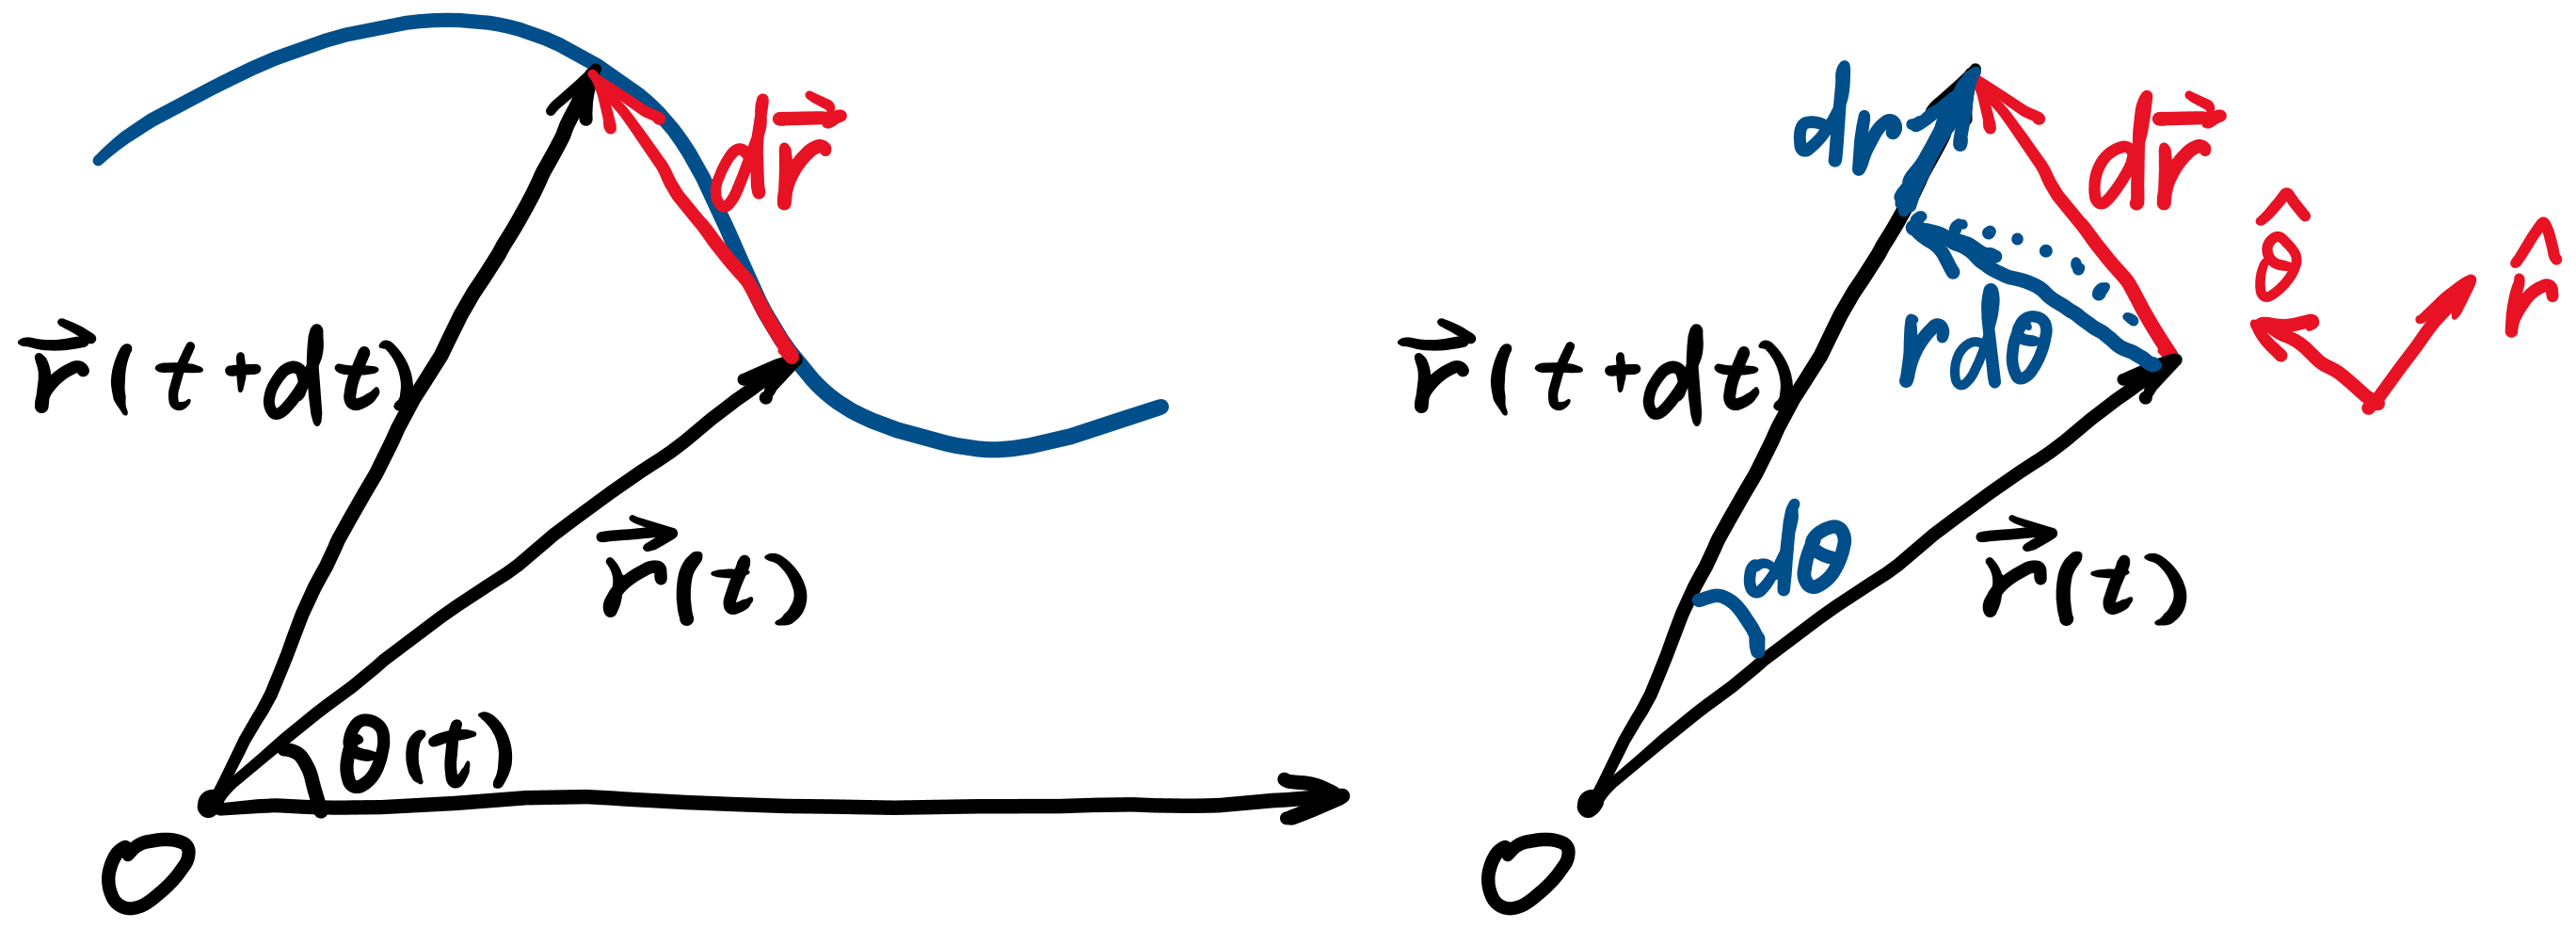
\includegraphics[width=8cm]{图片1.png}
		\captionof{figure}{在极坐标系下分解运动}\label{在极坐标系下分解运动}
	\end{center}
	\vspace{-1em}
\end{figure}

\zhu[加速度的极坐标分解]{
	在极坐标系中,对上面求出的$\vv = \dot{r}\ur + r\dot{\theta}\uq$再求一次导数,得
	\begin{align*}
		\voa = \dot{\vv} = \dt\left(\dot{r}\ur + r\dot{\theta}\uq\right)
		= \ddot{r}\ur + \dot{r}\dt[\ur] + \dot{r}\dot{\theta}\uq + r\ddot{\theta}\uq + r\dot{\theta}\dt[\uq]
	\end{align*}
	这引导我们考虑求$\dt[\ur]$和$\dt[\uq]$。观察知,有$\dif \ur = \dif \theta \uq$,$\dif \uq = -\dif \theta \ur$,即有$\dt[\ur] = \dot{\theta} \uq$,$\dt[\uq] = -\dot{\theta} \ur$。则 
	\begin{align*}
		\voa &= \ddot{r}\ur + \dot{r}\dt[\ur] + \dot{r}\dot{\theta}\uq + r\ddot{\theta}\uq + r\dot{\theta}\dt[\uq]
		= \ddot{r}\ur + \dot{r}\dot{\theta} \uq + \dot{r}\dot{\theta}\uq + r\ddot{\theta}\uq + r\dot{\theta}\left(-\dot{\theta} \ur\right)\\[-3pt]
		&= \left(\ddot{r} - r\dot{\theta}^2\right) \ur + \left(2\dot{r}\dot{\theta} + r\ddot{\theta}\right)\uq
	\end{align*}
}

\subsubsection{简单的运动分析}

\begin{circum}
	\textbf{匀加速运动。}加速度$\voa$是常矢量,则
	\begin{align*}
		&\dt[\vv]=\voa \Longrightarrow \int \dif\vv =\int \voa \dif t \Longrightarrow \vv=\voa t+\v{C} \xLongrightarrow{\vv|_{t=0}=\vv_0} \vv=\voa t+\vv_0\\[-4pt]
		&\dt[\vr]=\vv=\voa t+\vv_0 \Longrightarrow \int\dif\vr = \int(\voa t+\vv_0)\dif t \Longrightarrow \vr=\frac{1}{2}\voa t^2+\vv_0 t+\v{C} \xLongrightarrow{\vr|_{t=0}=\vr_0} \vr=\frac{1}{2}\voa t^2+\vv_0 t+\vr_0
	\end{align*}
\end{circum}
\begin{eg}{抛体运动}
	加速度恒为$\voa=\v{g}$,运动轨道在$\pb{\vv_0}{\v{g}}$确定的竖直平面内。沿水平方向($x$)和竖直方向($y$)分解,得$\begin{cases}
		v_x(t) \equiv v_0\cos\theta,\\
		v_y(t) = v_0\sin\theta - gt,
	\end{cases}$最高点$y_\mathrm{max} = \dfrac{v_0^2 \sin^2\theta}{2g}$,轨迹方程为$y=x \tan \theta - \dfrac{gx^2}{2v_0^2 \cos^2 \theta}$。
\end{eg}


\begin{circum}
	\textbf{圆周运动。}径矢$\vr$是长度恒为$R$的矢量,记为$\v{R}$。
	
	由中学知识可知,$v=\dt[s]=\dfrac{R\dif\theta}{\dif t}=\omega R$。依旋转方向按右手定则定义$\v{\omega}$的方向,则有$\vv=\v{\omega} \cp \v{R}$。将加速度$\voa$沿径向(内法向$\vu*{n}$)和切向($\uq$)分解为$\voa = a_\uptau\uq + a_\mathrm{n}\vu*{n}$,则径向上同理也有$a_\mathrm{n}=\dfrac{\left|\dif \vv_\mathrm{n}\right|}{\dif t}=\dfrac{v\dif\theta}{\dif t}=\omega v=\omega^2 R =\dfrac{v^2}{R}$,即有$a_\mathrm{n}\vu*{n}=\v{\omega} \cp \vv$;切向上则有$a_\uptau =\dt[v]=\dfrac{R \dif \omega}{\dif t}=\alpha R$,依角速度改变方向按右手定则定义$\v{\alpha}$的方向,则有$a_\uptau\uq=\v{\alpha} \cp \v{R}$。事实上,我们有
	$$\voa = \dt[\vv] = \dt (\v{\omega} \cp \v{R}) = \dt\v{\omega} \cp \v{R} + \v{\omega} \cp \dt\v{R} = \v{\alpha} \cp \v{R} + \v{\omega} \cp \vv$$
\end{circum}

\zhu[理解在转动上定义的矢量]{
	\hang 并非任意有大小有方向的物理量都可以定义为矢量。只有有方向且叠加(合成)遵循平行四边形法则的物理量才能定义为矢量。
	
	\hang 对转动矢量方向的定义必然涉及三维空间。质点转动可以看作对质点位矢的变换$\mathscr{R}$,对应于一个矩阵$\vb*{R}$。若有两个转动分别表示为矩阵$\vb*{M}=\vb*{I}+\varepsilon\vb*{m},\vb*{N}=\vb*{I}+\varepsilon\vb*{n}$,当转动角度无限小时$\varepsilon \to 0$,则这两个转动的叠加为
	$$\vb*{M}\vb*{N}=(\vb*{I}+\varepsilon\vb*{m})(\vb*{I}+\varepsilon\vb*{n})=\vb*{I} + \varepsilon(\vb*{m}+\vb*{n}) + \varepsilon^2\vb*{m}\vb*{n}$$
	因此,有限角转动(有限角位移)不是矢量,因为其叠加不满足交换律,必然不满足平行四边形定则;无限小角转动是矢量,因$\varepsilon \to 0$时上式最后高阶小项可忽略。无限小角转动的矢量方向由右手定则确定。

	\hang 事实上,对任意矢量$\v{A}$,若$A$不变,即$\v{A}$做旋转,设其角速度为$\v{\omega}$,则都有$\dot{\v{A}}=\v{\omega} \cp \v{A}$。
}

\subsubsection{相对运动}

\di[伽利略变换]{
	设参考系$S'$相对于参考系$S$平动的速度为$\v{u}$,一质点相对于$S'$的速度为$\vv'$,则该质点相对于$S$的速度为$\vv=\vv'+\v{u}$。
}

由结论~\ref{伽利略变换}~求导,即得$\dot{\vv}=\dot{\vv}'+\dot{\v{u}}$。当$S'$相对于$S$没有加速度时,即在惯性系之间,有$\dot{\vv}=\dot{\vv}'$;当$S'$相对于$S$有加速度时,有$\dot{\vv}'=\dot{\vv}-\dot{\v{u}}$,这个加速度便对应于后面所谓\textbf{惯性力}。

\subsection{牛顿运动定律}
\begin{abstract}
	\item[牛顿定律] 惯性系下,总成立:
		\begin{itemize}[leftmargin=3em, labelsep=0.25em, itemindent=0em, itemsep=0pt, parsep=0pt, topsep=0pt, partopsep=0pt]
			\item 牛顿第一定律(惯性定律):任何物体如果没有力的作用,都将保持静止的或作匀速直线运动的状态;

			\item 牛顿第二定律:物体所受的合外力$\v{F}=m\voa$;

			\item 牛顿第三定律:作用力与反作用力大小相等、方向相反,作用在不同物体上。
		\end{itemize}
	
	\item[量纲] 基本力学量长度、质量、时间的量纲分别记为L、M、T,如$[\vv]=\mathrm{LT^{-1}}$,$[\v{F}]=\mathrm{LMT^{-2}}$。
	
	\item[惯性力] $\v{F}_{\mathrm{i}}=-m\voa_0$,其中$\voa_0$是非惯性系的加速度。添加惯性力后,牛顿定律在非惯性系中成立。
	
	\item[惯性离心力] $\v{F}_\mathrm{cen} = m\omega^2\vr$,其中$\omega$是旋转参考系的角速度,$\vr$是旋转轴到物体的位矢。更一般地,$\v{F}_\mathrm{cen} =-m\v{\omega} \cp (\v{\omega} \cp \vr)$,其中$\v{\omega}$是旋转参考系的角速度,$\vr$是旋转轴上任意一点(取之为原点)到物体的位矢。
	
	\item[科里奥利力] $\v{F}_\mathrm{cor} = -2m \v{\omega} \cp \vv'$,其中$\v{\omega}$是旋转参考系的角速度,$\vv'$是质点相对旋转参考系的速度。
\end{abstract}

\subsubsection{牛顿定律与惯性系}

\di[牛顿定律]{
	\tbome{牛顿第一定律(惯性定律)}\hskip0.5em 任何物体如果没有力作用在它上面,都将保持静止的或作匀速直线运动的状态。

	\tbome{牛顿第二定律}\quad 物体所受的合外力等于其动量随时间的导数,即$\v{F}=\dt[\v{p}] \xlongequal{\frac{\dif m}{\dif t}=0} m\voa$。

	\tbome{牛顿第三定律}\quad 作用力与反作用力大小相等、方向相反,作用在不同物体上。	
}

\de[惯性系]{
	牛顿第一定律(惯性定律)成立的参考系是\tboba{惯性系}。
}
牛顿第一定律定义了惯性系,而牛顿第二、三定律只在惯性系中成立。

\begin{corollary}
	凡相对已知惯性系作匀速直线运动的参考系也是惯性系,而相对已知惯性系作加速运动的参考系为非惯性系;在一个参考系中,只要某个物体符合惯性定律,则其它物体都服从惯性定律。
\end{corollary}

因此,对某一特定物体惯性定律成立的参考系就是惯性系。\textbf{惯性不是个别物体的性质,而是参考系,或者说,时空的性质。}

\de[量纲式]{
	\hang 为定性表示导出量和基本量间的关系,常不考虑关系式中的数字因数,而将物理量用若干基本量的乘方之积表示,这样的式子称为该物理量的\tboba{量纲式},简称\tboba{量纲}。某物理量 $Q$的量纲通常表示为$[Q]$。

	基本力学量长度、质量、时间的量纲分别记为L、M、T。
}

可知$[\vv]=\mathrm{LT^{-1}}$,$[\v{F}]=\mathrm{LMT^{-2}}$等等。量纲分析可以检验计算结果。

\zhu[常见力与基本自然力]{
	自然界四种基本相互作用如表~\ref{四种基本相互作用}~所示。
	\begin{center}
		\vspace{-1em}
		\captionof{table}{四种基本相互作用}\label{四种基本相互作用}
		\vspace{1em}
		\begin{tabular}{p{75pt}<{\centering}p{75pt}<{\centering}p{60pt}<{\centering}p{60pt}<{\centering}p{75pt}<{\centering}}
			\toprule
			\textbf{作用} & \textbf{作用范围/m} & \textbf{长程行为} & \textbf{相对强度} & \textbf{现有理论} \\
			\midrule
			万有引力 & $\infty$ & $r^{-2}$ & 1 & 广义相对论 \\
			电磁相互作用 & $\infty$ & $r^{-2}$ & $10^{36}$ & 量子电动力学 \\
			弱相互作用 & $10^{-17}$ & $r^{-2}\e^{-mr}$ & $10^{25}$ & 电弱理论 \\
			强相互作用 & $10^{-15}$ & 1 & $10^{38}$ & 量子色动力学 \\
			\bottomrule
		\end{tabular}
	\end{center}
}

\subsubsection{非惯性系与惯性力}

地面参考系有$a_\text{自转} \sim \SI{3.4}{cm/s^2}$的自转加速度,
地心参考系有$a_\text{公转} \sim \SI{0.6}{cm/s^2}$的公转加速度,
若考虑这些加速度,则它们都是非惯性系。

由结论~\ref{伽利略变换}~的推论$\dot{\vv}'=\dot{\vv}-\dot{\v{u}}$,即有$m\voa'=m\voa-m\voa_0$,其中$\voa$是质点相对于惯性系$S$的加速度,$\voa'$是质点相对于非惯性系$S'$的加速度,$\voa_0$是非惯性系$S'$相对于惯性系$S$的加速度。在惯性系$S$中由牛顿第二定律,质点受到的合力为$\v{F}=m\voa$。为使牛顿第二定律在非惯性系$S'$中\textbf{形式上成立},引入
\de[惯性力]{
	设有非惯性系$S'$相对于惯性系$S$的加速度是$\voa_0$,则假想其中质量为$m$的物体额外受到$\v{F}_0=-m\voa_0$的力,可使牛顿第二定律在非惯性系$S'$中形式上成立,这个力$\v{F}_0=-m\voa_0$称为非惯性系$S'$中的\tboba{惯性力}。
}
\noindent 此时有$$\v{F}+\v{F}_0=m\voa'$$

\begin{example}[3]
	平面上有一斜面,其上有一物体自由下滑。忽略所有摩擦,求物体加速度。
	\begin{center}
		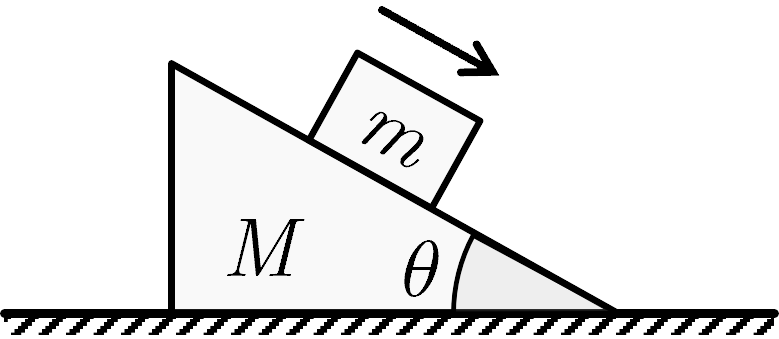
\includegraphics[width=3cm]{图片2.png}
	\end{center}
\begin{solution}[解法一]
	如图所示在地面上建系。
	\begin{center}
		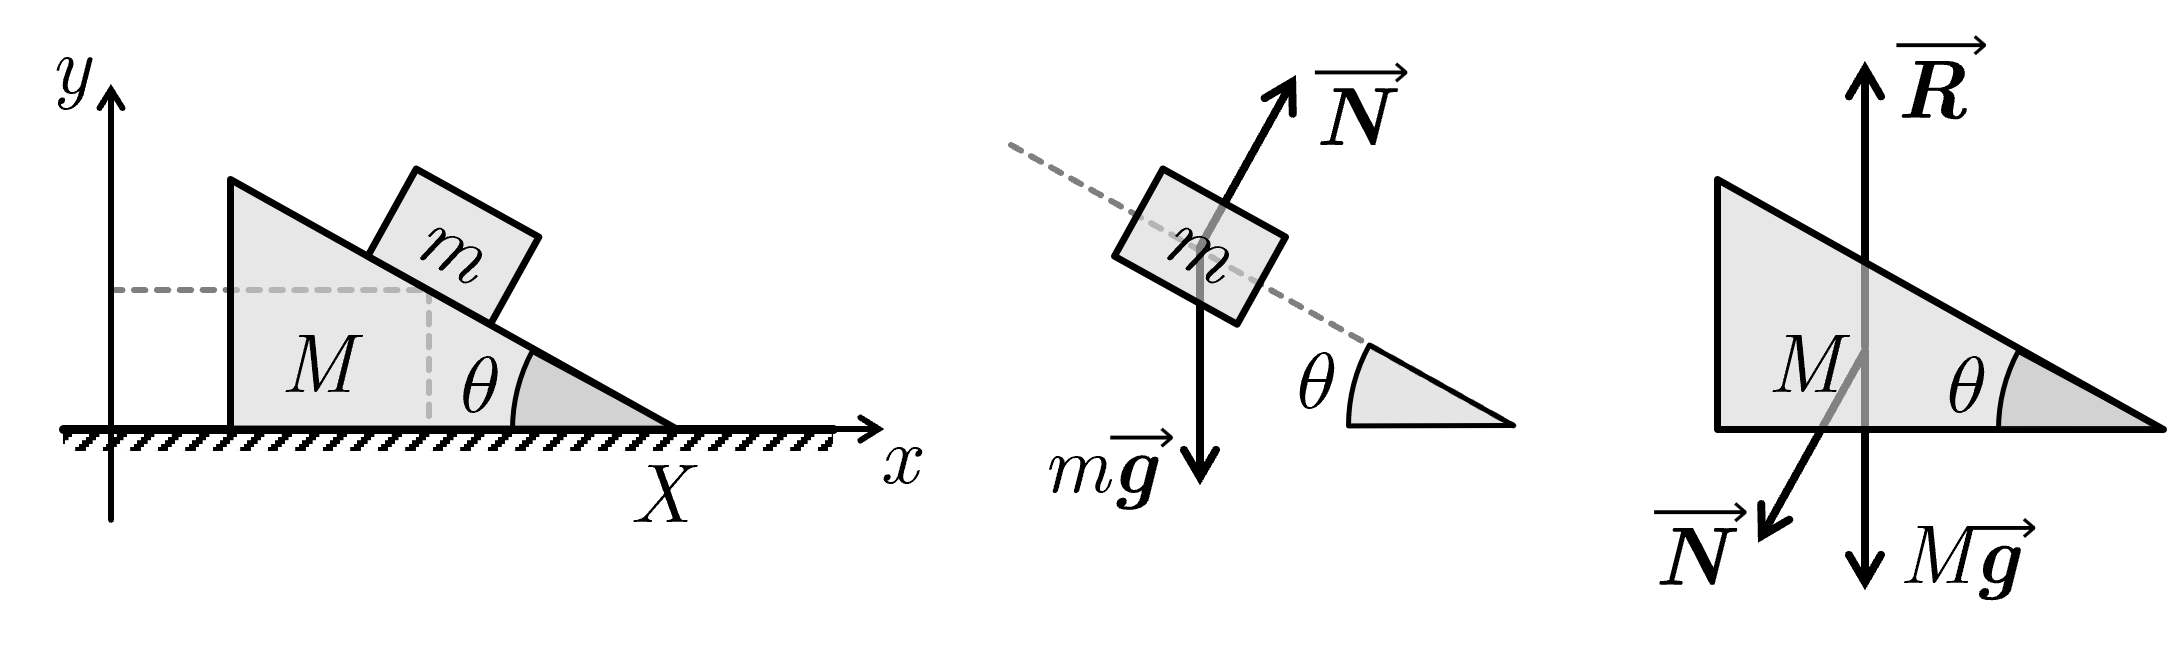
\includegraphics[width=8.35cm]{图片3.png}
		\vspace{-0.5em}
	\end{center}
	由牛顿第二定律,有
	$\begin{cases}
		N\cos\theta - mg = ma_y, \\
		N\sin\theta = ma_x, \\
		-N\sin\theta = MA\text{;}
	\end{cases}$
	由位置关系,有$y=(X-x)\tan \theta$,求二阶导得$a_y=(A-a_x)\tan \theta$。联立以上四式,解得
	$\begin{cases}
		a_x=\dfrac{Mg\sin\theta \cos\theta}{M+m\sin^2 \theta}, \\[6pt]
		a_y=-\dfrac{(M+m)g\sin^2\theta}{M+m\sin^2\theta}, \\[6pt]
		A=-\dfrac{mg\sin\theta\cos\theta}{M+m\sin^2\theta}\text{。}
	\end{cases}$
\end{solution}
\begin{solution}[解法二]
	如图所示,对物体的分析在斜面上建系,此为非惯性系。
	\begin{center}
		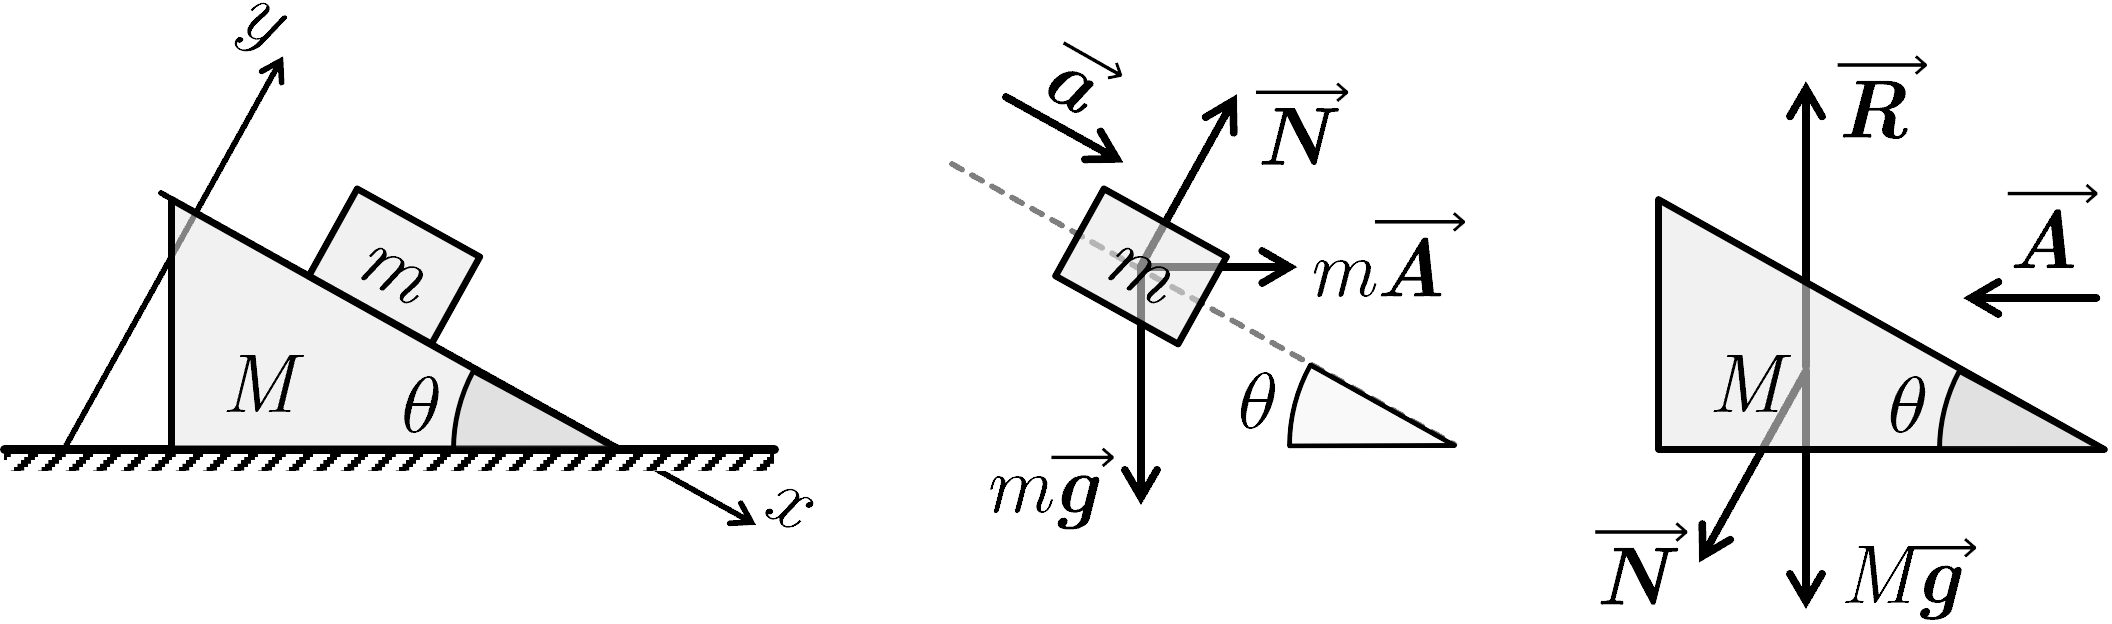
\includegraphics[width=8.13cm]{图片4.png}
	\end{center}
	由(形式上的)牛顿第二定律,有
	$\begin{cases}
		N + mA\sin\theta = mg\cos\theta, \\
		mg\sin\theta + mA\cos\theta = ma, \\
		N\sin\theta = MA,
	\end{cases}$解得
	$\begin{cases}
		a=\dfrac{(M+m)g\sin\theta}{M+m\sin^2 \theta}, \\[6pt]
		A=-\dfrac{mg\sin\theta\cos\theta}{M+m\sin^2\theta}\text{。}
	\end{cases}$
\end{solution}
\end{example}

\subsubsection{转动参考系中的离心力和科里奥利力}

\paragraph{惯性离心力}

若物体相对于转动参考系静止在距转轴的位矢为$\vr$,转动参考系的转动角速度是$\omega$,则在转动参考系中其受到惯性力$\v{F}_\mathrm{i} = m\omega^2\vr$,这个惯性力称为\tboba{离心力}。


\begin{eg}{地球自转离心力与地表重力加速度}

	如图~\ref{Pic: 地球表面重力加速度},地球表面重力加速度$\v{g}$是地表万有引力加速度$\voa_\text{引}$与离心加速度$\voa_\text{离}$的和,有
	$$g^2 = a_\text{引}^2 + a_\text{离}^2 - 2a_\text{引}a_\text{离}\sin\theta$$
	注意到$a_\text{引} \gg a_\text{离}$,即有
	\begin{align*}
	g = a_\text{引} \sqrt{1 + \left(\dfrac{a_\text{离}}{a_\text{引}}\right)^2 - 2\sin\theta \cdot \dfrac{a_\text{离}}{a_\text{引}}}
	\xlongequal{\frac{a_\text{离}}{a_\text{引}} \to 0} a_\text{引} \left(1 - \dfrac{a_\text{离}}{a_\text{引}}\sin\theta \right)= a_\text{引} - a_\text{离}\sin\theta
	\end{align*}

	\begin{center}
		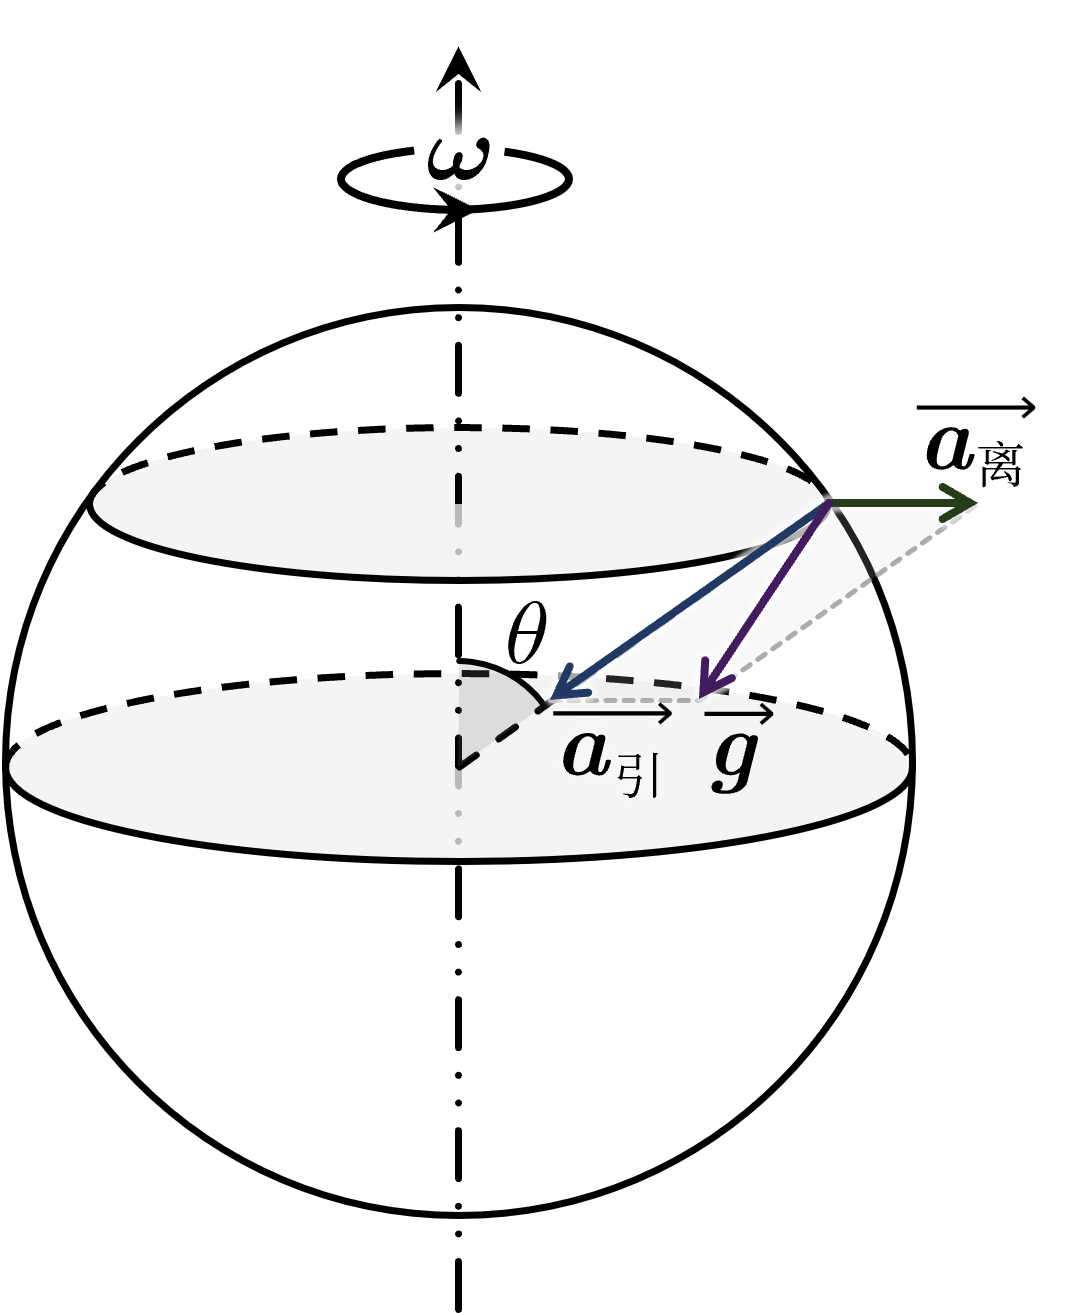
\includegraphics[width=4cm]{图片7.png}
		\captionof{figure}{地球表面重力加速度}\label{Pic: 地球表面重力加速度}
	\end{center}
\end{eg}

\begin{example}
	求以$\omega$角速度旋转的水面形状。
\begin{solution}
	在旋转参考系上建立柱坐标系,任选水面一小质元,其在切线方向静止,在此旋转参考系中
	$$mg\cos \theta - m\omega^2r \sin\theta = 0 
	\quad\Longrightarrow\quad \dfrac{\dif z }{\dif r } = \cot\theta = \dfrac{\omega^2r}{g}$$
	设水面该质元的柱坐标为$(z_v,r_v)$,其中$z$轴上水面位置为$z_0$,于是积分得
	\begin{equation*}
		\int_{z_0}^{z_v} \dif z = \int_0^{r_v} \dfrac{\omega^2r}{g} \dif r 
	\end{equation*}
	即
	\begin{equation*}
		z_v = z_0 + \dfrac{\omega^2r^2}{2g}
		\qedhere
	\end{equation*}

	\begin{center}
		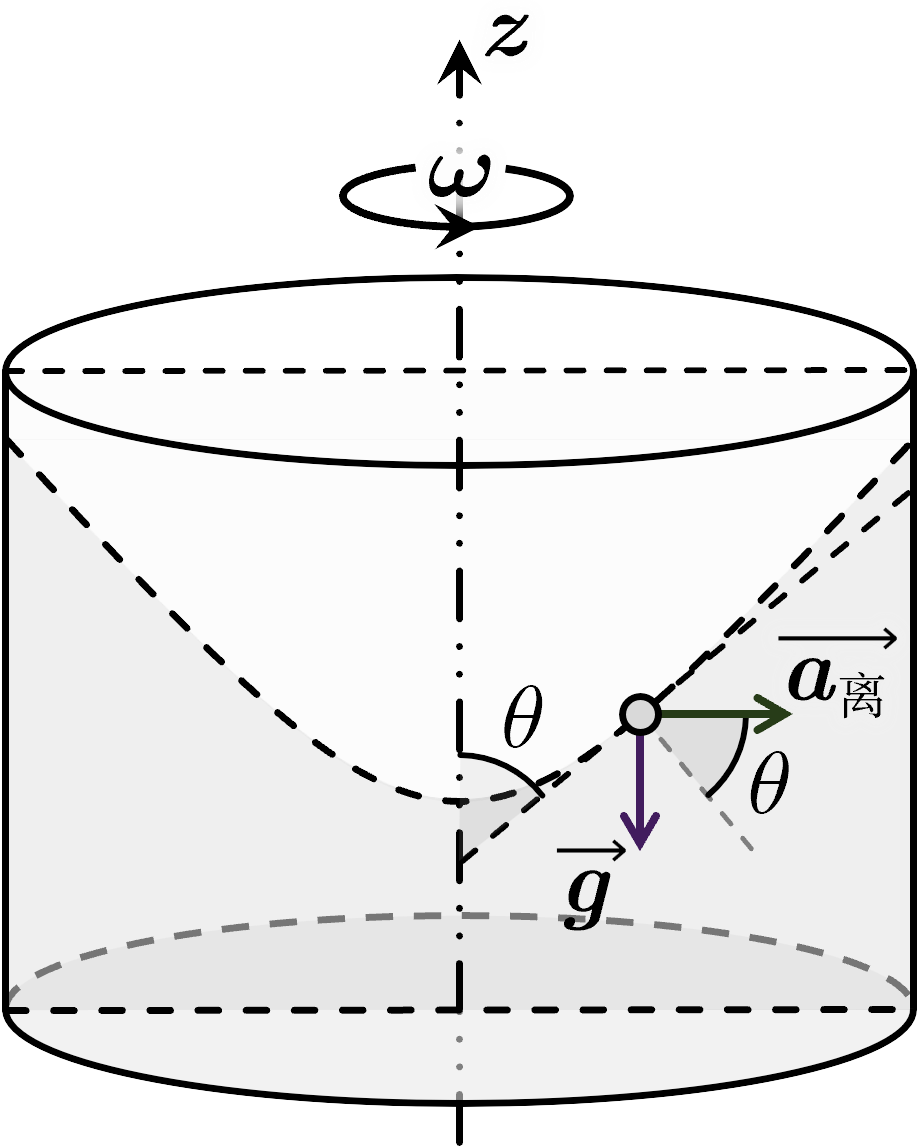
\includegraphics[width=3.53cm]{图片8.png}
	\end{center}
\end{solution}
\end{example}

\paragraph{科里奥利力}

设有惯性参考系$S(\vu*{\imath},\vu*{\jmath},\vu*{k})$,转动参考系$S'(\vu*{\imath}',\vu*{\jmath}',\vu*{k}')$以角速度$\omega$绕$S,S'$公共原点转动。对一个质点的位矢$\vr$,应有
\begin{align*}
	\vr &\xlongequal{S} x\vu*{\imath} + y\vu*{\jmath} + z\vu*{k}\\[-7pt]
	\vr &\xlongequal{S'} x'\vu*{\imath}' + y'\vu*{\jmath}' + z'\vu*{k}'
\end{align*}
对时间$t$求导,注意到$\vu*{\imath}',\vu*{\jmath}',\vu*{k}'$均是时间的函数,应有
\begin{align*}
	%\vv = \dot\vr &\xlongequal{S} v_x\vu*{\imath} + v_y\vu*{\jmath} + v_z\vu*{k}\\[-7pt]
	\vv = \dot\vr &\xlongequal{S'} v_x'\vu*{\imath}' + x'(\v{\omega} \cp \vu*{\imath}') + v_y'\vu*{\jmath}' + y'(\v{\omega} \cp \vu*{\jmath}') + v_z'\vu*{k}' + z'(\v{\omega} \cp \vu*{k}')\\[-7pt]
	&= \vv' + \v{\omega} \cp \vr\\[-4pt]
	%\voa = \dot\vv &\xlongequal{S} a_x\vu*{\imath} + a_y\vu*{\jmath} + a_z\vu*{k}\\[-7pt]
	\voa = \dot\vv &\xlongequal{S'} \dot\vv' + \v{\omega} \cp \dot\vr = \voa' + \v{\omega} \cp \vv' + \v{\omega} \cp (\vv' + \v{\omega} \cp \vr)\\[-7pt]
	&= \voa' + 2\v{\omega} \cp \vv' + \v{\omega} \cp (\v{\omega} \cp \vr)
\end{align*}
其中,$\vv' = v_x'\vu*{\imath}' + v_y'\vu*{\jmath}' + v_z'\vu*{k}' = \dot{r}_x'\vu*{\imath}' + \dot{r}_y'\vu*{\jmath}' + \dot{r}_z'\vu*{k}'$为质点在$S'$系下的速度,$\voa' = a_x'\vu*{\imath}' + a_y'\vu*{\jmath}' + a_z'\vu*{k}' = \ddot{r}_x'\vu*{\imath}' + \ddot{r}_y'\vu*{\jmath}' + \ddot{r}_z'\vu*{k}'$为质点在$S'$系下的加速度;于是有
$$m\voa - m \cdot 2\v{\omega} \cp \vv' - m\v{\omega} \cp (\v{\omega} \cp \vr) = m\voa'$$
其中,$-m\v{\omega} \cp (\v{\omega} \cp \vr)$为离心力,$-2m \v{\omega} \cp \vv'$即为\tboba{科里奥利力}。

地球北半球科里奥利力的方向如图~\ref{Pic: 地球北半球科里奥利力的方向}~所示;经验上,北半球的科里奥利力总是偏向速度方向的右侧。

\begin{figure}[ht!]
	\begin{center}
		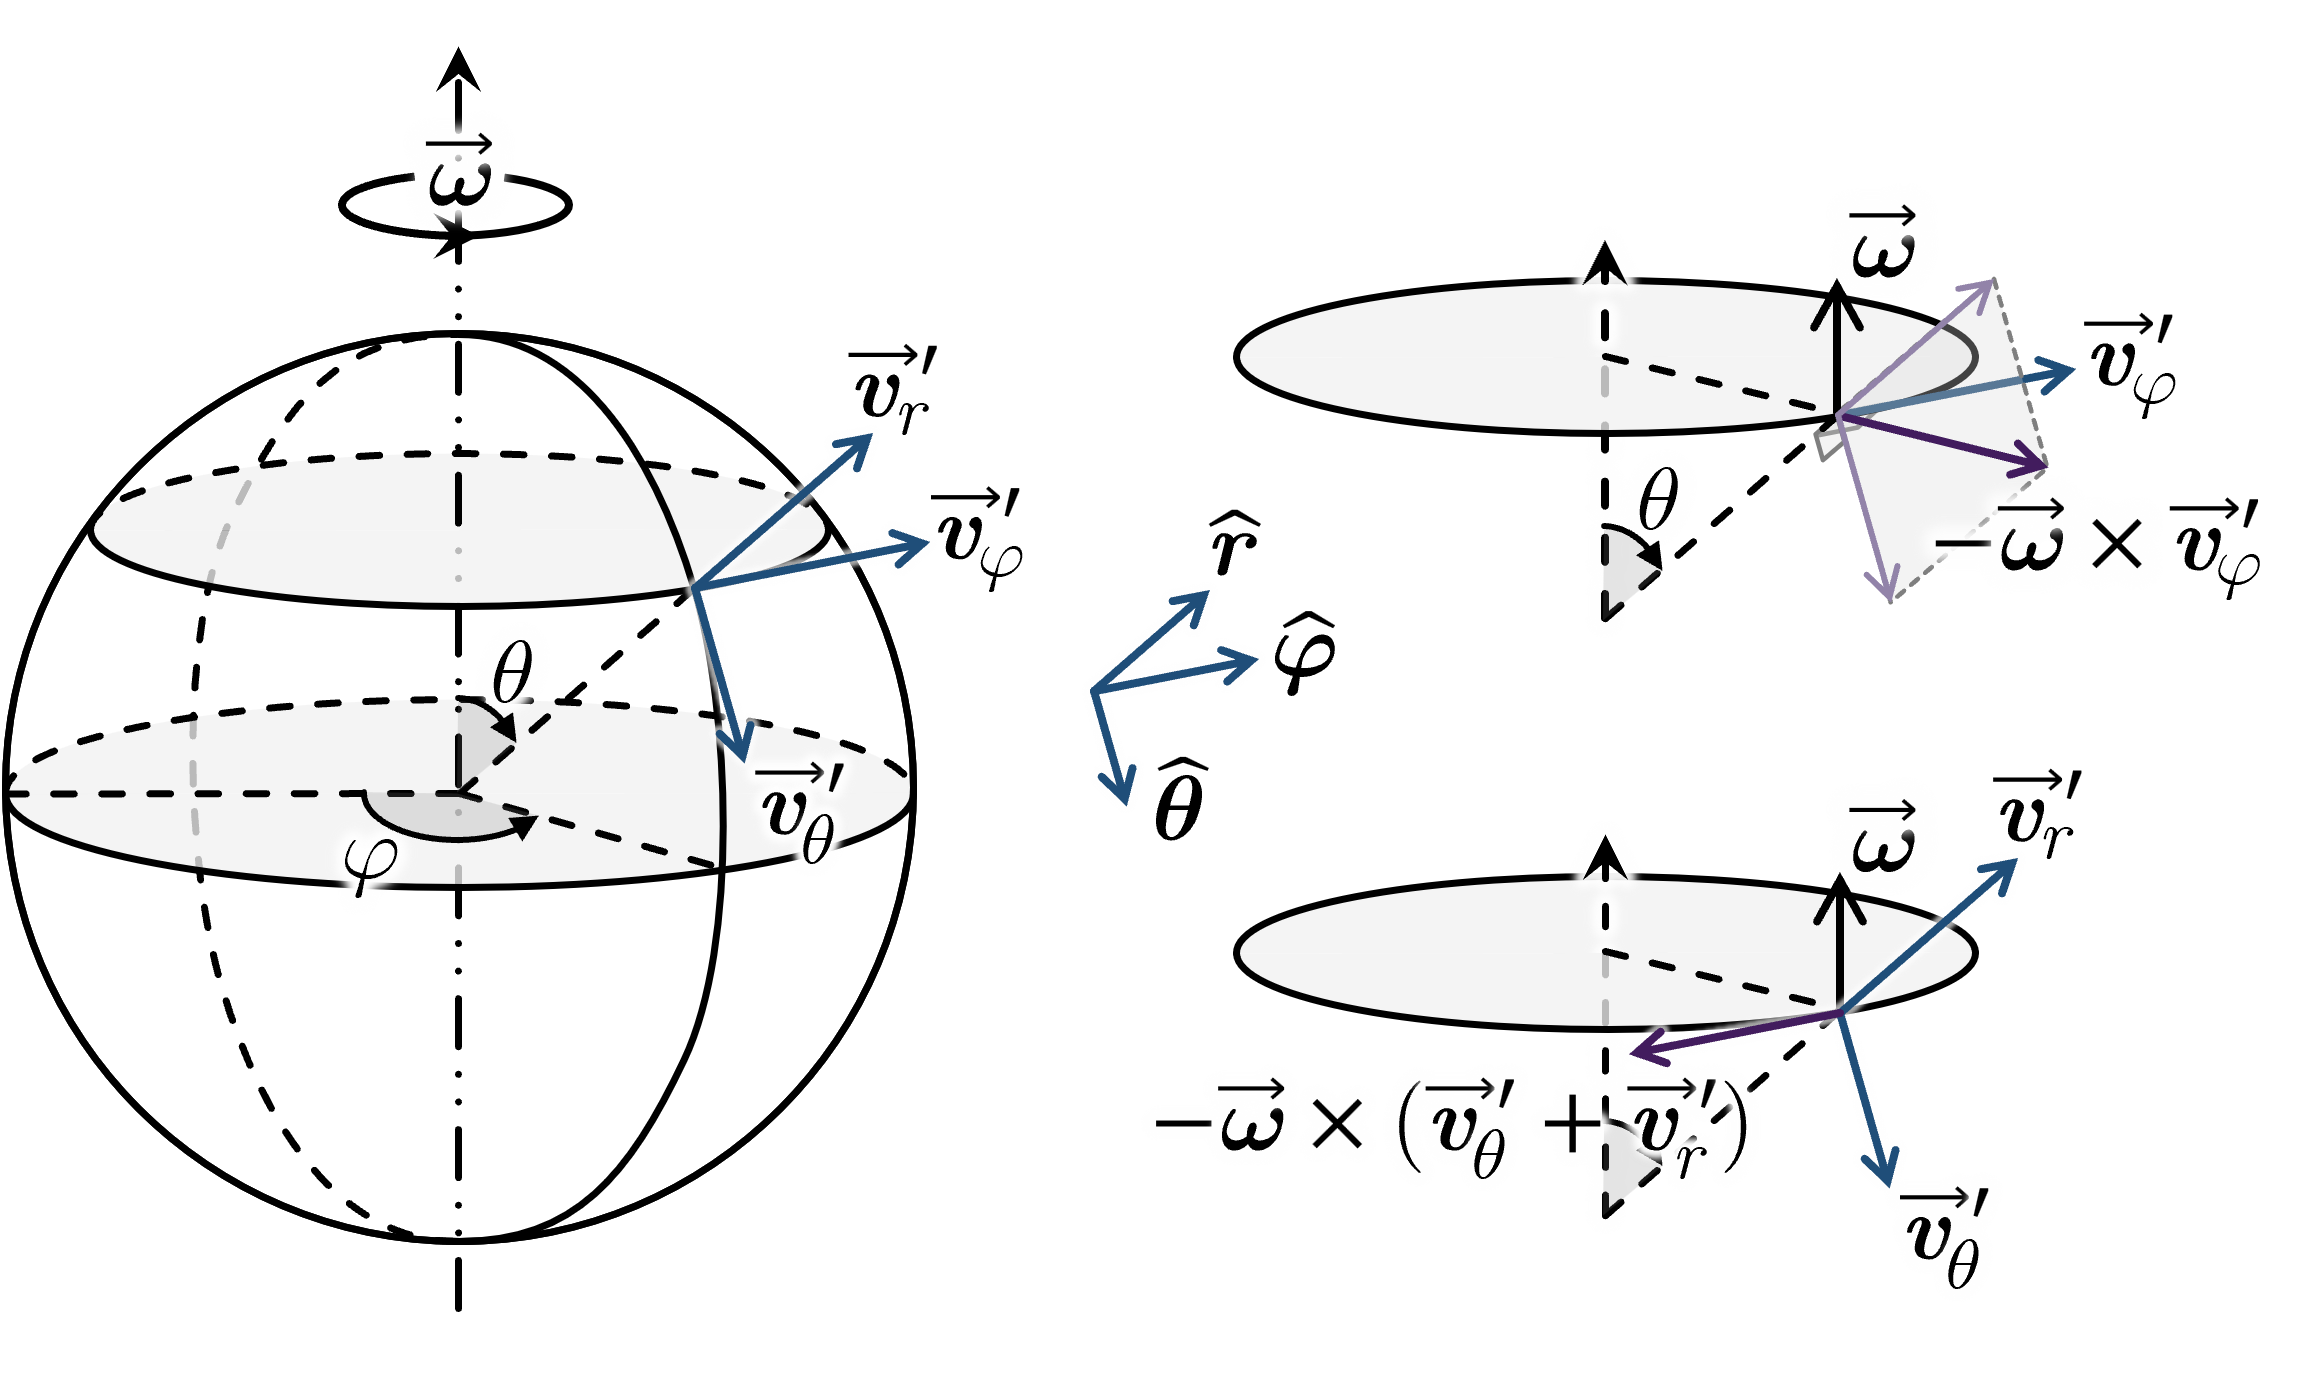
\includegraphics[width=8.75cm]{科里奥利力的方向.png}
		\caption{地球北半球科里奥利力的方向}\label{Pic: 地球北半球科里奥利力的方向}
		\vspace{-1em}
	\end{center}
\end{figure}

\begin{eg}{傅科摆}

	在地心参考系下,考虑地球表面的一个摆,如图~\ref{Pic: 傅科摆的计算}。$\v{\omega}$在$\left\{ \vu*{r}, \vu*{\theta} \right\} $平面内,分解为$\v{\omega} = \omega_{\parallel}\uq + \omega_{\perp}\vu*{r}$。
	
	将摆的运动近似看成在$\left\{ \vu*{\varphi}, \vu*{\theta} \right\} $平面内的运动,那么上式中,$\omega_{\parallel}$项在质点沿地表运动时产生的科里奥利力垂直于地表,只考虑$\omega_{\perp}$项。科里奥利力提供的加速度为
	\abovedisplayskip=2pt
	\belowdisplayskip=2pt
	$$\voa_{\mathrm{cor}} = -2\omega_{\perp}\vu*{r} \cp \vv' = -2 \omega \cos\theta \,\vu*{r} \cp \vv'$$
	即摆在地面系的水平面内运动方程为
	$$m\ddot{\v{r}}'=-\frac{mg}l\v{r}'-2m\omega \cos\theta \,\vu*{r} \cp \dot{\v{r}}'$$
	转写到地面极坐标系中,由分解$\dot{\vr}' = \dot{r}'\ur' + r'\dot{\gamma}\vu*{\gamma}$,$\ddot{\vr}' = \left(\ddot{r}' - r'\dot{\gamma}^2\right) \ur' + \left(2\dot{r}'\dot{\gamma} + r'\ddot{\gamma}\right)\vu*{\gamma}$,
	即有上式中$\vu*{r} \cp \dot{\v{r}}'= \vu*{r} \cp \left(\dot{r}'\ur' + r'\dot{\gamma}\vu*{\gamma}\right) = \dot{r}' \vu*{\gamma} - r'\dot{\gamma} \vu*{r}'$,于是
	$$\begin{cases}[ll]
		\vu*{r}'\colon & m\left(\ddot{r}' - r'\dot{\gamma}^2\right) = -\dfrac{mgr'}{l} +2m\omega \cos\theta\,  r'\dot{\gamma}, \\
		\vu*{\gamma}'\colon & m\left(2\dot{r}'\dot{\gamma} + r'\ddot{\gamma}\right) = -2m\omega \cos\theta\, \dot{r}'
	\end{cases}$$
	取$\ddot{\gamma}=0$的边界条件,即有
	$ \dot{\gamma} = -\omega \cos\theta$,
	进而傅科摆的摆动平面的转动周期为
	$$T=\frac{2\uppi}{\left|\dot{\gamma}\right|} = \frac{2\uppi}{\omega |\cos\theta|} = \frac{T_\mathrm{E}}{|\cos\theta|}$$
	即,傅科摆的摆动平面的转动方向与半球有关,周期与维度有关。极点处转动速度最快,周期为$T_\mathrm{E}$,即在地心参考系下摆动平面没有运动;赤道上转动周期为$\infty$,即在地面参考系下摆动平面没有转动。
	\begin{center}
		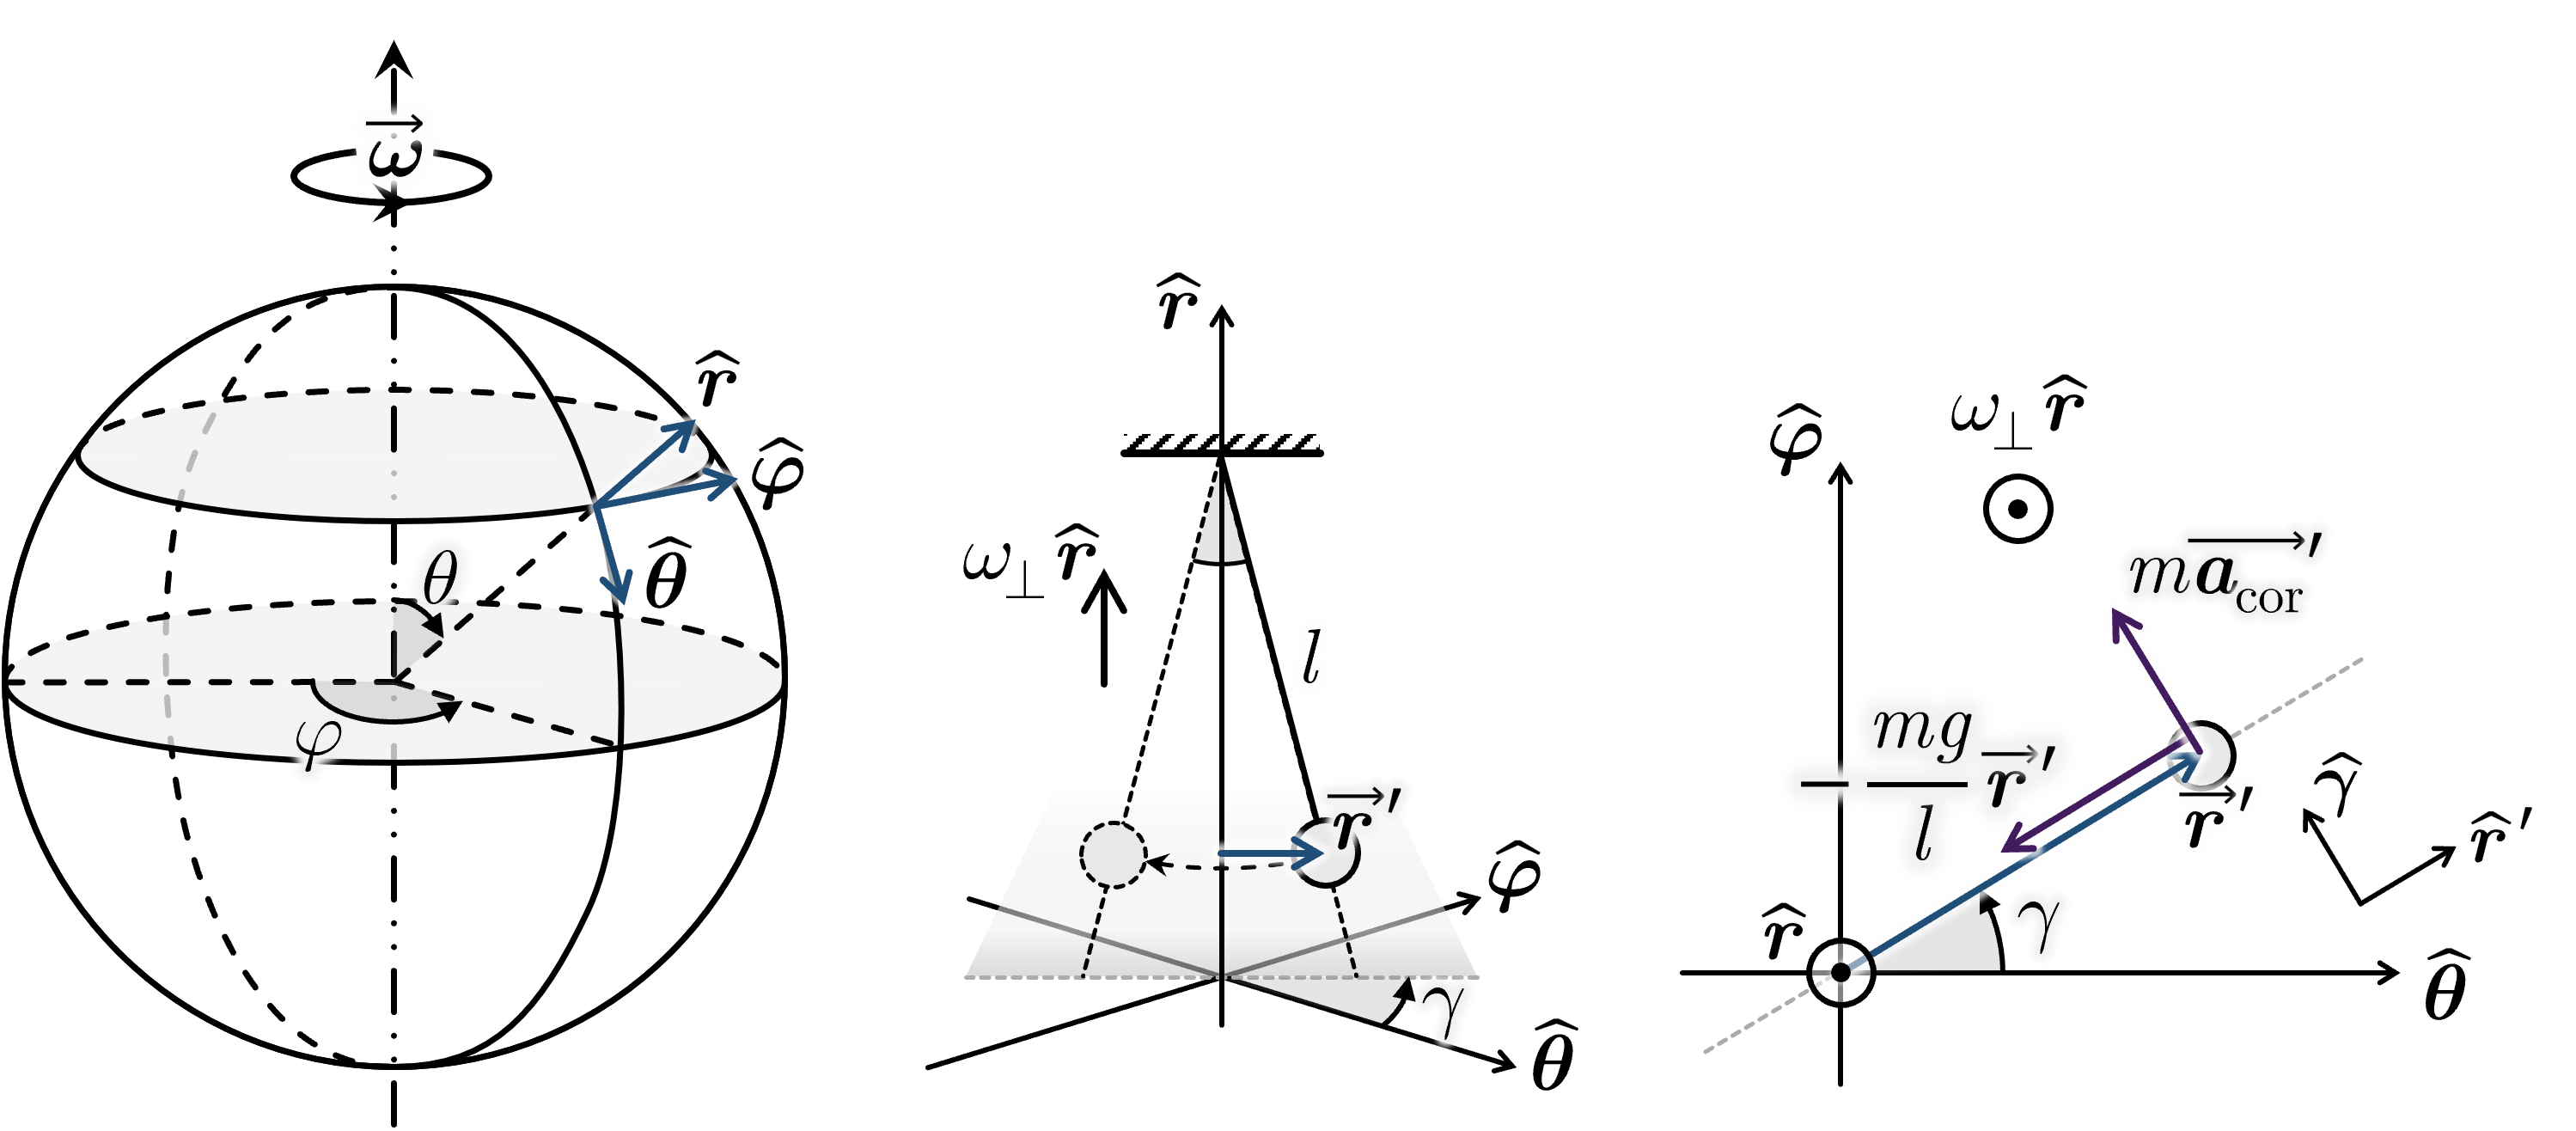
\includegraphics[width=11.61cm]{傅科摆.png}
		\captionof{figure}{傅科摆的计算}\label{Pic: 傅科摆的计算}
	\end{center}
\end{eg}

\Subsubsection{一个复杂实例:潮汐}



\subsection{动量与角动量}
\begin{abstract}
	\item[动量定理] 惯性系下,总成立:
	\begin{itemize}[leftmargin=3em, labelsep=0.25em, itemindent=0em, itemsep=0pt, parsep=0pt, topsep=0pt, partopsep=0pt, ]
		\item 质点动量定理:物体所受的合外力等于其动量随时间的导数,即$\v{F}=\dt[\v{p}]$。
		
		\item 质点系动量定理:在一个质点系中,设其质点$i$所受的来自质点系外的力之合力为$\v{F}_i$,$\sum\limits_i \v{F}_i = \v{F}_\text{外}$,动量为$\v{p}_i$,$\sum\limits_i \v{p}_i = \v{P}$,则有 $\v{F}_\text{外}=\dt[\v{P}]$。
	\end{itemize}

	\item[质点系动量守恒定律] 若质点系所受合外力为零,则质点系的总动量不随时间改变。
	
	\item[力矩] $\v{M}=\v{r}\cp \v{F}$。
	\item[角动量]  $\v{L}=\v{r} \cp \v{p}$。
	
	\item[角动量定理] 相对于惯性系中的定点$O$,总成立:
	\begin{itemize}[leftmargin=3em, labelsep=0.25em, itemindent=0em, itemsep=0pt, parsep=0pt, topsep=0pt, partopsep=0pt]
		\item 质点角动量定理:质点所受合力的力矩,等于质点的角动量随时间的导数,即$\v{M} = \dt[\v{L}]$。
		
		\item 质点系角动量定理:记质点系中质点$i$所受的来自质点系外的力之合力矩为$\v{M}_i$,$\sum\limits_i \v{M}_i = \v{M}_\text{外}$,角动量为$\v{L}_i$,$\sum\limits_i \v{L}_i = \v{L}$,则有 $\v{M}_\text{外}=\dt[\v{L}]$。
	\end{itemize}

	\item[质点系角动量守恒定律] 若质点系所受合外力矩为零,则质点系的总角动量不随时间改变。

	\item[质心] $N$个质点组成质点系的质心位置为$\vr_c = \dfrac{\sum\limits_{i=1}^N m_i\vr_i}{\sum\limits_{i=1}^N m_i} = \dfrac{\sum\limits_{i=1}^N m_i\vr_i}{M}$。
	\begin{itemize}[leftmargin=3em, labelsep=0.25em, itemindent=0em, itemsep=0pt, parsep=0pt, topsep=0pt, partopsep=0pt]
		\item 质心运动定律:设质点系所受合外力为$\v{F}$,总质量为$M$,质心的加速度为$\voa_c$,则$\v{F} = M \voa_c$。

		\item 质心系动量守恒定律:质心系下该质点系的总动量恒为$\v{0}$。
		
		\item 质心系角动量变换定理:质点系对惯性系定点$O$的角动量,等于质心对该定点的角动量加上质点系对质心的角动量。
		
		\item 质心系角动量定理:质点系各质点所受外力对质心的合力矩,等于质点系对质心的角动量的变化率。
	\end{itemize}
\end{abstract}
\subsubsection{力与动量}
\de[冲量]{
	力$\v{F}(t)$在$t_1$到$t_2$时间内的\tboba{冲量}定义为$\v{I} = \dint_{t_1}^{t_2} \v{F}(t) \dif t$。
}
\de[动量]{
	质量为$m$、速度为$\vv$的质点的\tboba{动量}定义为$\v{p} = m \vv$。
}
\di[质点动量定理]{
	物体所受的合外力等于其动量随时间的导数,即$\v{F}=\dt[\v{p}]$。

	\tbome{微分形式}\quad $\dif \v{I} = \v{F} \dif t = \dif \v{p}$。

	\tbome{积分形式}\quad $\v{I} = \dint_{t_1}^{t_2} \v{F}(t) \dif t = \v{p}_2 - \v{p}_1$。
}
\begin{eg}{逆风行舟}
	「熟练的水手」可以控制风帆的弧度,使得前侧向来风经过风帆后速度指向正后方,空气的动量变化量指向后侧方,使船获得向前的力。
	\begin{center}
		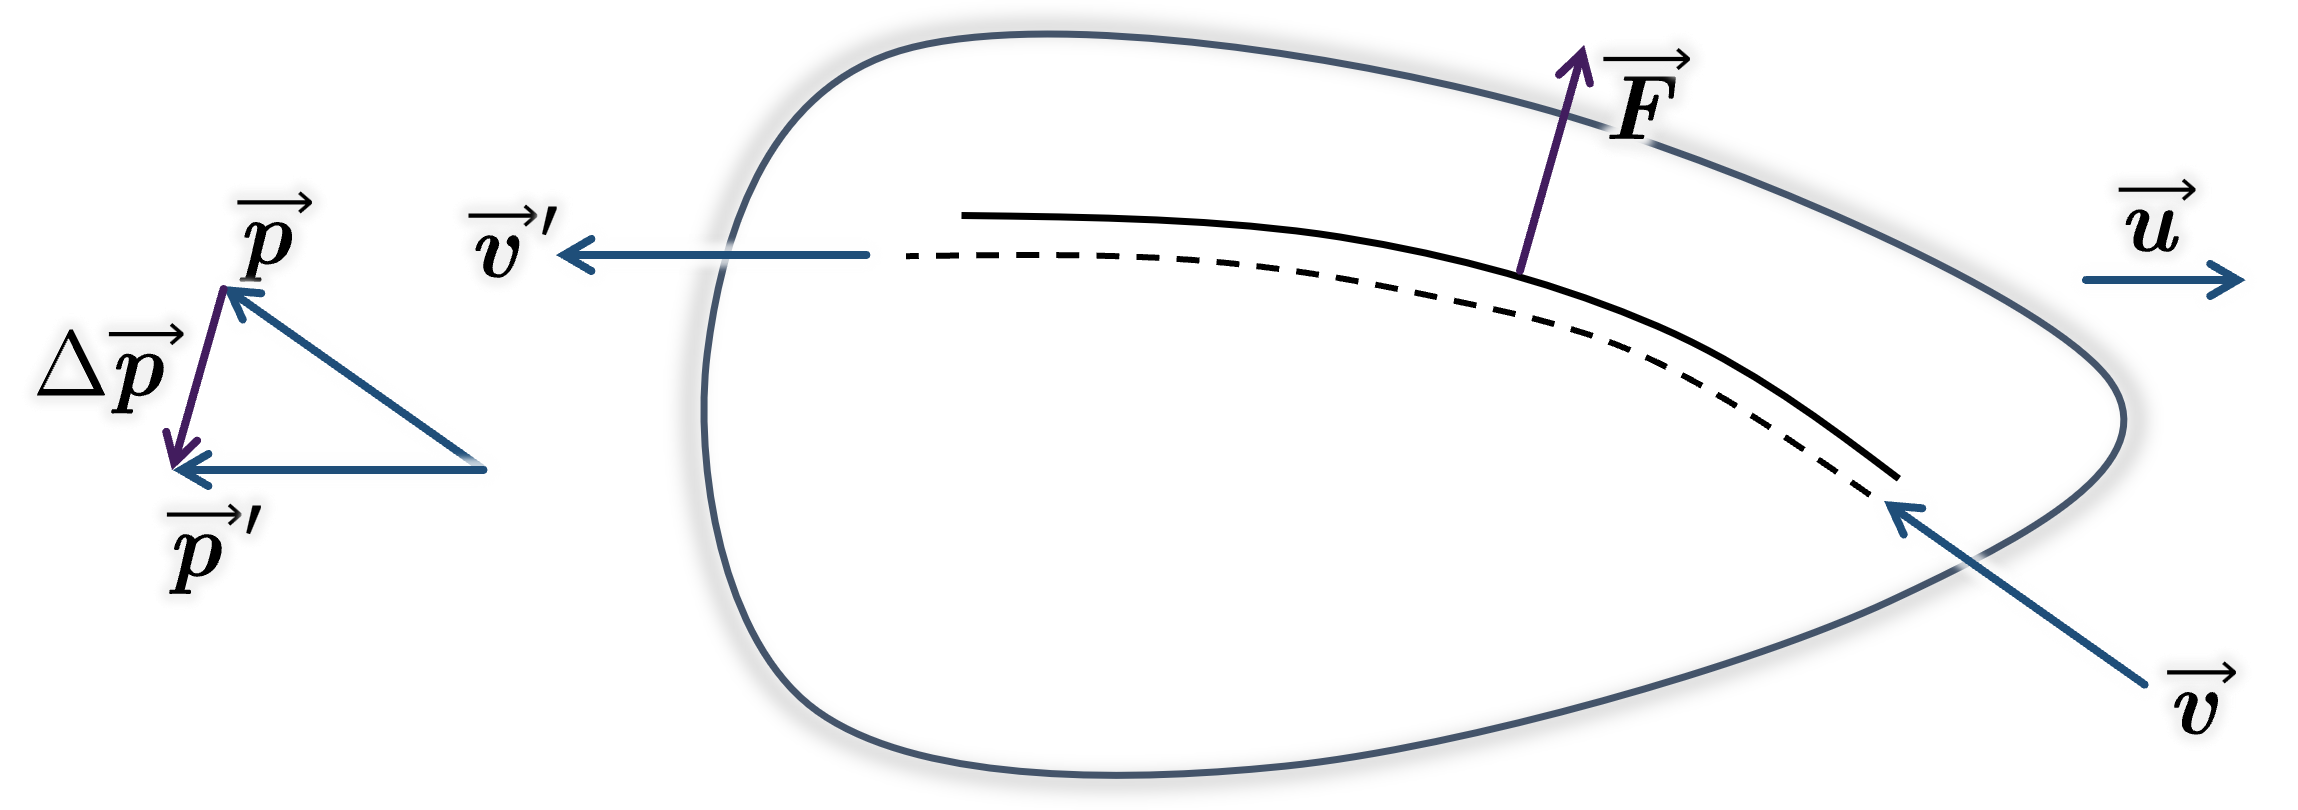
\includegraphics[width=8.95cm]{逆风行舟.png}
	\end{center}
\end{eg}
\di[质点系动量定理]{
	在一个质点系中,设其质点$i$所受的来自质点系外的力之合力为$\v{F}_i$,动量为$\v{p}_i$。记$\sum\limits_i \v{F}_i = \v{F}_\text{外}$,$\sum\limits_i \v{p}_i = \v{P}$,则有 $\v{F}_\text{外}=\dt[\v{P}]$。

	\tbome{微分形式}\quad $\dif \v{F}_\text{外} \dif t = \dif \v{P}$。

	\tbome{积分形式}\quad $\dint_{t_1}^{t_2} \v{F}_\text{外}(t) \dif t = \v{P}_2 - \v{P}_1$。
	
}
\begin{example}
	一柔软绳长$l$,线密度$\rho$,一端着地开始自由下落,求下落任意时刻给地面的压力。
\begin{solution}
	以地面为原点,竖直向上建立坐标系,记下落任意时刻绳顶端位置为$y$,$\eval{y}_{t=0} = l$。
	\abovedisplayskip=2pt
	\belowdisplayskip=2pt
	由质点系动量定理,$$ N - \rho l g = \dot{p}$$
	而$p = \rho y v$,即 $$\dot{p} = \rho \dt[(yv)] = \rho \left(\dot{y}v + y \dot{v}\right) = \rho \left(v^2 - yg\right) $$
	又由$v^2 = 2g(l-y)$,全部代入就有
	\begin{equation*}
		N = \rho l g + \dot{p} = \rho l g + \rho \left(v^2 - yg\right) = \rho l g + \rho \left(2g(l-y) - yg\right) = 3\rho g(l-y) \qedhere
	\end{equation*}
\end{solution}
\end{example}
\begin{eg}{火箭飞行}
	对火箭,$t$时刻的动量$\v{p} = M\vv$。经$\dif t$时间喷出$\dif m$的燃料,其相对火箭的速度为$\v{u}$,系统总动量为$\v{p}(t+\dif t) = (M-\dif m)(\vv+\dif \vv) + \dif m(\vv + \v{u})$,于是有
	$$ \dif \v{p} = M\dif \vv + \v{u} \dif m $$
	而由动量定理有$M\v{g} = \dt[\v{p}]$,则$M\v{g} = M\dt[\vv] + \v{u} \dt[m]$。而$\dif m = -\dif M$,则$M\v{g} = M\dt[\vv] - \v{u} \dt[M]$,即 
	$$ \v{g}\dif t + \v{u} \dfrac{\dif M }{M} = \dif \vv $$
	则 
	$$ \int_{t_\mathrm{i}}^{t_\mathrm{f}} \v{g}\dif t + \int_{M_\mathrm{i}}^{M_\mathrm{f}} \v{u} \dfrac{\dif M }{M} = \int_{\vv_\mathrm{i}}^{\vv_\mathrm{f}} \dif \vv $$
	即
	$$ \vv_\mathrm{f} - \vv_\mathrm{i} = \v{g}(t_\mathrm{f}-t_\mathrm{i}) + \v{u} \ln\dfrac{M_\mathrm{f}}{M_\mathrm{i}} $$
\end{eg}

\di[质点系动量守恒定律]{
	若质点系所受合外力为零,则质点系的总动量不随时间改变。
}
外力与内力相比小很多(如烟花的重力与其空中爆炸的冲击力)的情况下,也可忽略外力,近似看作质点系动量守恒。
\de[质点系的质心]{
	定义$N$个质点组成质点系的\tboba{质心}位置为$\vr_c = \dfrac{\sum\limits_{i=1}^N m_i\vr_i}{\sum\limits_{i=1}^N m_i} = \dfrac{\sum\limits_{i=1}^N m_i\vr_i}{M}$。

	对连续分布的物质,质心位置为$\vr_c = \dfrac{\dint_\mathcal{O} \vr_i\dif m}{\dint_\mathcal{O} \dif m} = \dfrac{\dint_\mathcal{O} \vr_i\dif m}{M}$。
}
以质心为参考建立质心系,则有$\sum\limits_{i=1}^N m_i\vr_i'=\sum\limits_{i=1}^N m_i(\vr_i-\vr_c) = \v{0}$。由此求导即有$\sum\limits_{i=1}^N m_i\vv_i' = \v{0}$,即
\di[质心系动量守恒定律]{
	质心系下该质点系的总动量恒为$\v{0}$。
}
\di[质心运动定律]{
	设质点系所受合外力为$\v{F}$,总质量为$M$,质心的加速度为$\voa_c$,则$\v{F} = M \voa_c$。
}
\begin{proofs}
	$\v{P} = \sum\limits_{i=1}^N \v{p}_i = \sum\limits_{i=1}^N m_i\dfrac{\dif \vr_i}{\dif t} = \dfrac{\dif \left(\sum\limits_{i=1}^N m_i\vr_i\right)}{\dif t} = \dfrac{\dif (M \vr_c)}{\dif t} = M\dfrac{\dif \vr_c}{\dif t} = M\vv_c$;$\v{F} = \dt[\v{P}]$。
\end{proofs}

\zhu[重心]{
	在地心参考系下,设有一物体受到地球引力为$\v{F} = \sum\limits_i \v{F}_i = -GM_\mathrm{E} \sum\limits_i \dfrac{\Delta m_i}{r_i^3}\vr_i$。取其质心$\vr_c$,有$\vr_i = \vr_c + \vr_i'$。由于$r_c \gg r_i'$,有 
	\begin{equation*}
		\frac{\v{r}_i}{r_i^3}
		=\frac{\v{r}_c+\v{r}_i'}{\left(r_c^2+{r'}_i^2+2\v{r}_c\cdot\v{r}_i'\right)^{3/2}}
		\approx\frac{\v{r}_c}{r_c^3}+\frac{1}{r_c^3}\left(\v{r}_i'-\frac{3\v{r}_c(\v{r}_c\cdot\v{r}_i')}{r_c^2}\right)
	\end{equation*}
	那么 
	\begin{equation*}
		\v{F} = -GM_\mathrm{E} \sum\limits_i \Delta m_i \left(\frac{\v{r}_c}{r_c^3}+\frac{1}{r_c^3}\left(\v{r}_i'-\frac{3\v{r}_c(\v{r}_c\cdot\v{r}_i')}{r_c^2}\right)\right)
	\end{equation*}
	而 $\sum\limits_{i=1}^N m_i\vr_i' = \v{0}$,则 
	\begin{equation*}
		\v{F} = -GM_\mathrm{E} \frac{\v{r}_c}{r_c^3} \sum\limits_i \Delta m_i = -G\frac{M_\mathrm{E}M_\mathcal{O}}{r_c^3} \v{r}_c 
	\end{equation*}
	也即,在\tboqi{物体线度远小于到地心的距离}时,可以认为重力作用于质心,即重心与质心重合。
}
\begin{circum}
	\textbf{两体问题。}\label{两体问题之一}考虑两个物体构成的体系(如地—月体系),惯性系下其内力的牛顿第二定律为
	$$\v{f}_{21} = m_1\voa_1, \qquad \v{f}_{12} = m_2\voa_2$$
	且知$\v{f}_{21} = - \v{f}_{12}$。二者之质心的加速度为$\voa_c = \dfrac{m_1\voa_1 + m_2\voa_2}{m_1 + m_2} = \v{0}$,记$m_2$相对$m_1$的加速度为$\voa = \voa_2 - \voa_1$,则可解出$\voa_1 = -\dfrac{m_2\voa }{m_1+m_2},\voa_2 = \dfrac{m_1\voa }{m_1+m_2}$,于是 
	$$\v{f}_{12} = \dfrac{m_1m_2}{m_1+m_2} \voa =: \mu \voa$$
	此处$\mu$称为\tboba{约化质量},满足$\mu^{-1} = m_1^{-1} + m_2^{-1}$。利用约化质量,可以将两体问题转化为单体问题。
\end{circum}
\subsubsection{力矩与角动量}
\de[力矩]{
	设力$\v{F}$作用位置相对于原点$O$的位矢为$\vr$,则这个力相对于$O$的\tboba{力矩}定义为$\v{M} = \vr \cp \v{F}$。
}
由前面的讨论同理可知,重力相对于质点系重心(质心)的力矩为$\v{0}$。
\de[角动量]{
	设质点以动量$\v{p}$运动,相对于原点$O$的位矢为$\vr$,则这个质点相对于$O$的\tboba{角动量}定义为$\v{L} = \vr \cp \v{p}$。
}
\di[质点角动量定理]{
	质点所受合力相对于$O$的力矩,等于质点相对于$O$的角动量随时间的导数,即$\v{M} = \dt[\v{L}]$。

	\tbome{微分形式}\quad $\v{M} \dif t = \dif \v{L}$。

	\tbome{积分形式}\quad $\dint_{t_1}^{t_2} \v{M}(t) \dif t = \v{L}_2 - \v{L}_1$。
}
\begin{proofs}
	$\dot{\v{L}} = \dt[(\vr \cp \v{p})] = \dot{\vr} \cp \v{p} + \vr \cp \dot{\v{p}} \xlongequal[\dot{\v{p}} = \v{F}]{\dot{\vr} \parallel \v{p}} \vr \cp \v{F} = \v{M}$。
\end{proofs}

\di[质点系角动量定理]{
	在一个质点系中,相对于一固定点$O$,设其质点$i$所受的来自质点系外的力之合力矩为$\v{M}_i$,角动量为$\v{L}_i$。记$\sum\limits_i \v{M}_i = \v{M}_\text{外}$,$\sum\limits_i \v{L}_i = \v{L}$,则有 $\v{M}_\text{外}=\dt[\v{L}]$。

	\tbome{微分形式}\quad $\dif \v{M}_\text{外} \dif t = \dif \v{L}$。

	\tbome{积分形式}\quad $\dint_{t_1}^{t_2} \v{M}_\text{外}(t) \dif t = \v{L}_2 - \v{l}_1$。
}
\di[质点系角动量守恒定律]{
	若质点系所受合外力矩为零,则质点系的总角动量不随时间改变。
}
\begin{corollary}
	\textbf{开普勒第二定律}\quad 若质点相对点$O$所受合力矩为零,则从$O$引出到该质点的位矢单位时间扫过的面积相同。
\end{corollary}
\begin{proofs}
	角动量恒为$\v{L}$,$L = mvr\sin\left\langle \vr, \vv \right\rangle = m \dfrac{\left|\dif \vr\right|}{\dif t}r\sin\left\langle \vr, \dif \vr \right\rangle = 2m \dfrac{\frac{1}{2}\left|\dif \vr\right|r\sin\left\langle \vr, \dif \vr \right\rangle}{\dif t} = 2m \dt[S] $。
\end{proofs}

与重力看作所有质量集中于质心类似,也可以将质点系的重力矩看作质量集中于质心产生的重力矩,即$\sum\limits_{i=1}^N \vr_i \cp m_i\v{g} = \sum\limits_{i=1}^N m_i\vr_i \cp \v{g} = M\vr_c \cp \v{g} = \vr_c \cp M \v{g}$。进而,质点系相对于自身质心的重力矩为$\v{0}$。

\di[质心系角动量变换定理]{
	质点系对惯性系定点$O$的角动量,等于质心对该定点的角动量(称为\tbome{轨道角动量})加上质点系对质心的角动量。
}
\di[质心系角动量定理]{
	质点系各质点所受外力对质心的合力矩,等于质点系对质心的角动量的变化率。
}
\begin{proofs}
	\adjline
	在质心系下,
	\begin{align*}
		\v{L} &= \sum_i \vr_i \cp \v{p}_i 
		= \sum_i \left(\vr_i'+\vr_c\right) \cp m_i \left(\vv_i'+\vv_c\right) \\[-4pt]
		&= \sum_i \vr_i' \cp \v{p}_i' + \underbrace{\sum_i m_i\vr_i'}_{\v{0}} \cp \vv_c + \vr_c \cp \underbrace{\sum_i \v{p}_i'}_{\v{0}} + \vr_c \cp \sum_i m_i\vv_c \\[-4pt]
		&= \v{L}' + \vr_c \cp \v{P}
	\end{align*}
	式中$\v{L}'$是质点系对质心的合角动量,$\v{P}$是质点系相对于惯性系中点$O$的动量(或称质心的动量),$\vr_c \cp \v{P}$即是轨道角动量。

	相对定点$O$,质点系各质点所受外力的合力矩为
	\begin{align*}
		\v{M} &= \sum_i \vr_i \cp \v{F}_i 
		= \sum_i \left(\vr_i'+\vr_c\right) \cp \v{F}_i
		= \sum_i \vr_i' \cp \v{F}_i+\vr_c \cp \sum_i \v{F}_i \\[-20pt]
		|| \ & \\[-8pt]
		\dt[\v{L}] &= \dt\left(\v{L}' + \vr_c \cp \v{P}\right) = \dt[\v{L}'] + \dt[\vr_c] \cp \v{P} + \vr_c \cp \dt[\v{P}] 
		\xlongequal{\vv_c \parallel \v{P}} \dt[\v{L}'] + \vr_c \cp \dt[\v{P}]
	\end{align*}
	而$\dt[\v{P}] = \sum_i \v{F}_i$,于是有$$\v{M}' = \sum_i \vr_i' \cp \v{F}_i = \dt[\v{L}']$$
	其中$\v{M}'$即是质点系各质点所受力相对质心的合力矩。
\end{proofs}
注意,结论~\ref{质点系角动量定理}~只在$O$是惯性系中定点时成立,而结论~\ref{质心系角动量定理}~没有对质心的运动情况做出要求。这与结论~\ref{质点系动量守恒定律}~和结论~\ref{质心系动量守恒定律}~的关系类似。
\begin{example}[2]
	光滑平面上,质量均为 $M$ 的两小球由一长为 $l$ 的轻杆相连,另一个质量为 $m$ 的小球与某一 $M$ 发生完全弹性碰撞,碰后 $m$ 沿垂直于原速度方向运动,如图所示。所有小球的大小可以忽略。试问:

    (1)若以碰撞点为原点,则相对原点碰撞前后系统角动量是否守恒?碰撞瞬间杆的另一端 $M$(没有与$m$直接碰撞)的速度方向?

    (2)令$m=M$,$\theta = 45^\circ$,求碰撞后$m$的速度 和轻杆系统绕其质心转动的角速度。
\begin{center}
	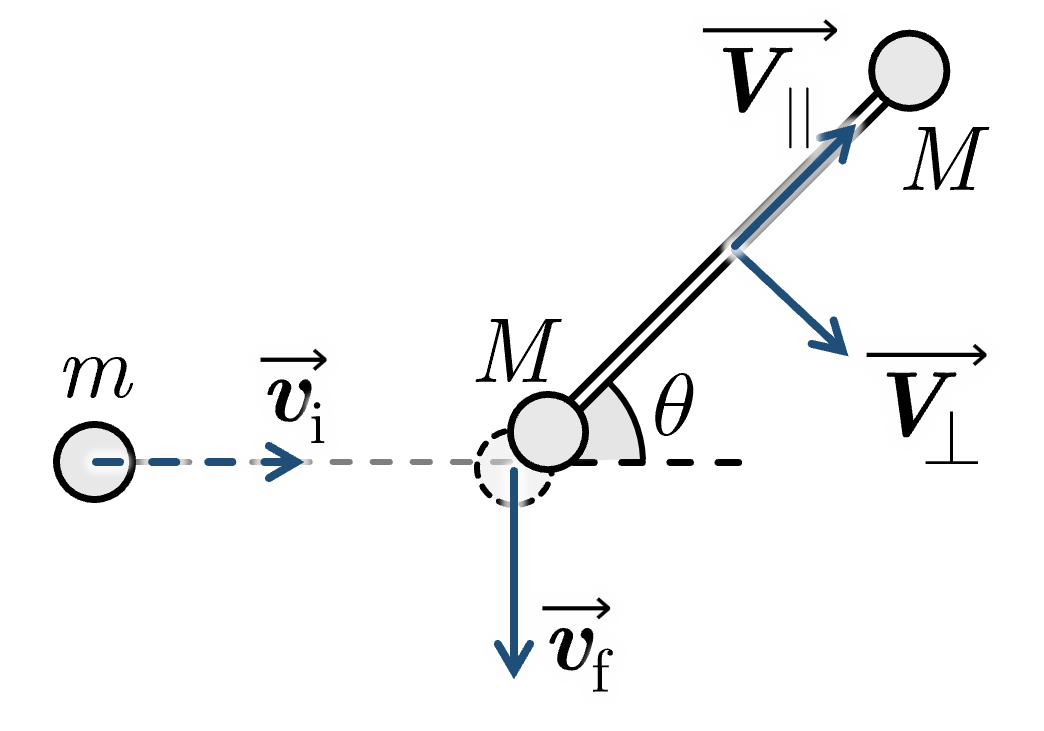
\includegraphics[width=3.81cm]{图片12.png}
	\vspace{-1em}
\end{center}
\begin{solution}
	\adjline
	(1)没有外力,角动量守恒(且均为$\v{0}$);杆只能给另一端$M$沿杆方向的力,则另一端 $M$的速度方向沿杆。

	(2)将杆系统质心速度沿平行、垂直于质心与碰撞点连线方向分解为$\v{V}\!_c=\v{V}\!_\parallel+\v{V}\!_\perp$。由(1),整个系统碰后角动量为$\v{0}$,而$m$速度反向延长线过碰撞点,则杆系统角动量相对碰撞点为$\v{0}$。于是由质心系角动量变换定理有
	\begin{equation*}
		\v{0} = - 2M \cdot \frac{1}{2}l \cdot V_\perp + 2M \cdot \frac{1}{2}l \cdot \frac{1}{2}l\omega  \quad\Longrightarrow\quad  \omega = \frac{2V_\perp}{l}
	\end{equation*}
	由动量守恒和能量守恒
	\begin{equation*}
		\begin{cases}
			mv_\mathrm{i}\cos\theta = 2MV_\parallel - mv_\mathrm{f}\sin\theta, \\[-1pt]
			mv_\mathrm{i}\sin\theta = 2MV_\perp + mv_\mathrm{f}\cos\theta,\\[1pt]
			\dfrac{1}{2}mv_\mathrm{i}^2 = \dfrac{1}{2}\cdot 2M V_\parallel^2 + \dfrac{1}{2}\cdot 2M V_\perp^2 + \dfrac{1}{2}mv_\mathrm{f}^2 
		\end{cases}
	\end{equation*}
	于是解出$v_\mathrm{f}=\pm\dfrac{\sqrt{3}}{3}v_\mathrm{i},V_\parallel=\dfrac{3\sqrt{2} \pm \sqrt{6}}{12}v_\mathrm{i},V_\perp=\dfrac{3\sqrt{2} \mp \sqrt{6}}{12}v_\mathrm{i}$,则$\omega = \dfrac{3\sqrt{2} \mp \sqrt{6}}{6l}v_\mathrm{i}$。
\end{solution}
\end{example}

\subsection{功和能}
\begin{abstract}
	\item[动能定理] 惯性系中,总成立
	\begin{itemize}[leftmargin=3em, labelsep=0.25em, itemindent=0em, itemsep=0pt, parsep=0pt, topsep=0pt, partopsep=0pt]
		\item 质点动能定理:合外力对质点所做的功等于质点动能的增量,即$w_{AB}=E_{\mathrm{k}B} - E_{\mathrm{k}A}$。
		\item 质点系动能定理:质点系各质点所受外力与内力做功之和,等于这段运动始末质点系总动能之差。
	\end{itemize}

	\item[柯尼希定理] 质点系的总动能等于轨道动能和内动能之和,即$E_{\mathrm{k}}=E_{\mathrm{k}c} + E_{\mathrm{k}}' $。
	\item[质心系动能定理] 质心参考系下,外力与内力对质点系做功之和,等于质点系总动能的变化量。
	\item[保守力与势能] 保守力是所做的功与路径无关、只与始末位置有关的一类力,其可与一类只与位置有关的能量联系起来,即势能。
	\begin{itemize}[leftmargin=3em, labelsep=0.25em, itemindent=0em, itemsep=0pt, parsep=0pt, topsep=0pt, partopsep=0pt]
		\item 引力势能$E_\mathrm{p}(r) = -G\dfrac{Mm}{r}$;弹性势能$E_\mathrm{p}(x)=\dfrac{1}{2}kx^2$。
		\item 直角坐标系下,保守力$\v{f}(x,y,z)$对应的势能函数$E_\mathrm{p}=E_\mathrm{p}(x,y,z)$,则 $\v{f} = -\nabla E_\mathrm{p}$。
	\end{itemize}
	\item[有心力场基本方程] 质点在势能函数为$V(r)$的有心力场中运动,满足
	$$\begin{cases}
		mr^2\dot{\theta} = L,\\
		\dfrac{1}{2}m\dot{r}^2 + \dfrac{L^2}{2mr^2} + V(r) = E,
	\end{cases} \qq{其中}\begin{cases}
		\v{L} = \vr_0 \cp m\vv_0, \\
		E = \dfrac{1}{2}m\vv_0^2 + V(r_0)
	\end{cases}$$
	\item[理想流体的稳定流动] 对稳定流动的理想流体,取其流线管中的一段,有
	\begin{itemize}[leftmargin=3em, labelsep=0.25em, itemindent=0em, itemsep=0pt, parsep=0pt, topsep=0pt, partopsep=0pt]
		\item 连续性方程:$v_1A_1 = v_2A_2$,即流量$Q=vA$为常量;
		\item 伯努利方程:$\dfrac{p_1 }{\rho_1} + \dfrac{1}{2}v_1^2 + U_1 = \dfrac{p_2 }{\rho_2} + \dfrac{1}{2}v_2^2 + U_2 $,即$\dfrac{p}{\rho} + \dfrac{1}{2}v^2 + U$为常量。
	\end{itemize}
\end{abstract}
\subsubsection{功和动能}
\de[功]{
	力$\v{F}$与力作用的物体在力作用下的位移$\Delta\v{r}$的点乘称为力在这段位移上对物体做的\tboba{功}。

	对变力$\v{F}$在一段路径$AB$上做的功,沿路径积分为$W_{AB}=\dint_\v{A}^\v{B} \v{F} \cdot \dif \vr$。
}
\di[质点动能定理]{
	合外力对质点所做的功等于质点动能的增量;即,质点在力$\v{f}$作用下从$\v{A}$运动到$\v{B}$,在两端的动能分别为$E_{\mathrm{k}A}$和$E_{\mathrm{k}B}$,那么力$\v{f}$做的功为$w_{AB}=E_{\mathrm{k}B} - E_{\mathrm{k}A}$。

	\tbome{微分形式}\quad $\dif\left(\dfrac{1}{2}mv^2\right) = \v{f}\cdot\dif \vr$。

	\tbome{积分形式}\quad $\dint_\v{A}^\v{B} \v{f}\cdot \dif\vr = E_{\mathrm{k}B} - E_{\mathrm{k}A}$。
}
\begin{proofs}
	$w_{AB}=\dint_\v{A}^\v{B} \v{f}\cdot \dif \vr
	=\dint_\v{A}^\v{B} m\dt[\vv]\cdot \dif \vr
	=\dint_{\vv_A}^{\vv_B} m\dif\vv \cdot \vv
	=\dint_{E_{\mathrm{k}A}}^{E_{\mathrm{k}B}} \dif\left(\dfrac{1}{2}m \vv \cdot \vv\right) = E_{\mathrm{k}B} - E_{\mathrm{k}A}$。
\end{proofs}

\di[质点系动能定理]{
	质点系各质点所受外力与内力做功之和,等于这段运动始末质点系总动能之差。
}
\begin{proofs}
	\adjline
	设惯性系下质点系中质点$i$所受合外力为$\v{F}_i$,所受质点$j$的力为$\v{f}_{ij}$,则对质点$i$就有
	\begin{equation*}
		w_i = \int_{\v{A}_i}^{\v{B}_i} \left(\v{F}_i + \sum_{j \neq i} \v{f}_{ij}\right)\cdot \dif\vr_i = E_{\mathrm{k}i}(\v{B}_i) - E_{\mathrm{k}i}(\v{A}_i)
	\end{equation*}
	则对这个质点系
	\begin{align*}
		E_{\mathrm{k}B}-E_{\mathrm{k}A}
		&= \sum_i E_{\mathrm{k}i}(\v{B}_i) - \sum_i E_{\mathrm{k}i}(\v{A}_i)
		= \sum_i \bigl(E_{\mathrm{k}i}(\v{B}_i) - E_{\mathrm{k}i}(\v{A}_i)\bigr) \\[-7pt]
		&= \sum_i \int_{\v{A}_i}^{\v{B}_i} \left(\v{F}_i + \sum_{j \neq i} \v{f}_{ij}\right)\cdot \dif\vr_i 
		= \sum_i \int_{\v{A}_i}^{\v{B}_i} \v{F}_i\cdot \dif\vr_i + \sum_i \int_{\v{A}_i}^{\v{B}_i} \sum_{j \neq i} \v{f}_{ij} \cdot\dif\vr_i \\[-7pt]
		&= W_\text{外} + W_\text{内}
		\qedhere
	\end{align*}
\end{proofs}

\di[柯尼希定理]{
	质点系的总动能等于质心的动能(称为\tbome{轨道动能})和内动能之和。

	即,设质点系中质点$i$的质量为$m_i$,速度为$\vv_i$,质点系质心的速度为$\vv_c$,质点$i$相对质心的速度为$\vv_i'$,记质点系总动能$E_\mathrm{k}=\sum\limits_{i} \dfrac{1}{2}m_i\vv_i^2$,轨道动能$E_{\mathrm{k}c} = \left(\sum\limits_{i} \dfrac{1}{2}m_i\right)\vv_c^2$,内动能$E_{\mathrm{k}}'=\sum\limits_{i} \dfrac{1}{2}m_i\vv_i'^2$,则
	$$E_{\mathrm{k}}=E_{\mathrm{k}c} + E_{\mathrm{k}}' $$
}
\begin{proofs}
	\adjline[10]
	设质点系质心的速度为$\vv_c$,质点系中质点$i$的速度为$\vv_i$,则质点系的总动能
	\begin{align*}
		E_{\mathrm{k}}' 
		&=\sum\limits_i \dfrac12 m_i(\vv_i-\vv_c)^2
		=\sum\limits_i \dfrac12 m_i\vv_i^2 - \underbrace{\sum\limits_i m_i\vv_i}_{\left(\sum\limits_i  m_i\right)\vv_c} \cdot\vv_c + \sum\limits_i \dfrac12 m_i\vv_c^2 \\[-12pt]
		&=\sum\limits_{i}\dfrac{1}{2}m_{i}\vv_{i}^{2}-\dfrac{1}{2}\left(\sum\limits_{i}m_{i}\right)\vv_{c}^{2}=E_{\mathrm{k}}-E_{\mathrm{k}c} \qedhere
	\end{align*}	
\end{proofs}
\begin{circum}
	\textbf{两体问题中的动能。}情形~\ref{两体问题之一}~已导出约化质量$\mu = \dfrac{m_1m_2}{m_1+m_2}$。设出质心系下两物体的速度$\vv_1'=\vv_1-\vv_c$,$\vv_2'=\vv_2-\vv_c$,则物体$m_2$相对$m_1$的速度$\vv=\vv_2-\vv_1=\vv_2'-\vv_1'$。又质心系是零动量参考系,有$m_1\vv_1' + m_2\vv_2' = \v{0}$,即可解出$\vv_1' = -\dfrac{m_2\vv }{m_1+m_2},\vv_2' = \dfrac{m_1\vv }{m_1+m_2}$,于是内动能\label{两体问题之二}
	\begin{equation*}
		\frac12 m_1v_1'^2 + \frac12 m_2v_2'^2 
		= \frac12 m_1\dfrac{m_2^2\vv^2 }{(m_1+m_2)^2} + \frac12 m_2\dfrac{m_1^2\vv^2 }{(m_1+m_2)^2} 
		= \dfrac{m_1m_2\vv^2 (m_1+m_2)}{2(m_1+m_2)^2}
		= \frac12 \dfrac{m_1m_2}{m_1+m_2} v^2
		= \frac12 \mu v^2
	\end{equation*}
	故由柯尼希定理,即有$E_{\mathrm{k}}=\dfrac{1}{2}Mv_c^2 + \dfrac{1}{2}\mu v^2$。
\end{circum}
\di[质心系动能定理]{
	质心参考系下,外力与内力对质点系做功之和,等于质点系总动能的变化量。
}
\begin{proofs}
	\adjline
	对质点系中质点$i$,我们有$\vr_i'=\vr_i-\vr_c$,进而设质点$i$所受合力为$\v{f}_i$,所受合外力为$\v{F}_i$即有
	\begin{align*}
		\v{f}_i \cdot \dif\vr_i = \v{f}_i \cdot \dif\vr_i' + \v{f}_i \cdot \dif\vr_c 
		&\Longrightarrow \sum_i \v{f}_i \cdot \dif\vr_i = \sum_i \v{f}_i \cdot \dif\vr_i' + \sum_i \v{f}_i \cdot \dif\vr_c \\[-7pt]
		&\Longrightarrow \sum_i \v{f}_i \cdot \dif\vr_i = \sum_i \v{f}_i \cdot \dif\vr_i' + \sum_i \v{F}_i \cdot \dif\vr_c \\[-7pt]
		&\Longrightarrow \int_{\v{A}_i}^{\v{B}_i} \sum_i \v{f}_i \cdot \dif\vr_i = \int_{\v{A}_i'}^{\v{B}_i'} \sum_i \v{f}_i \cdot \dif\vr_i' + \int_{\v{A}_c}^{\v{B}_c} \sum_i \v{F}_i \cdot \dif\vr_c \\[-7pt]
		&\Longleftrightarrow W_{\text{外},AB}+W_{\text{内},AB} = W_{\text{外},A'B'}+W_{\text{内},A'B'} + \int_{\v{A}_c}^{\v{B}_c} \sum_i \v{F}_i \cdot \dif\vr_c
	\end{align*}
	而由柯尼希定理,有 
	\begin{equation*}
		W_{\text{外},AB}+W_{\text{内},AB} = E_{\mathrm{k}B} - E_{\mathrm{k}A} = E_{\mathrm{k}cB} - E_{\mathrm{k}cA} + E_{\mathrm{k}B}' - E_{\mathrm{k}A}'
	\end{equation*}
	记质点系总质量为$M = \sum\limits_i m_i$,所受合外力为$\v{F} = \sum\limits_i \v{F}_i $,则
	\begin{equation*}
		\int_{\v{A}_c}^{\v{B}_c} \v{F} \cdot \dif\vr_c
		= \int_{\v{A}_c}^{\v{B}_c} M\dt[\vv_c] \cdot \dif\vr_c
		= \int_{\v{A}_c}^{\v{B}_c} M\dif \vv_c \cdot \dif\vv_c
		= \int_{\v{A}_c}^{\v{B}_c} \dif \left(\frac12 M\vv_c^2\right)
		= E_{\mathrm{k}cB} - E_{\mathrm{k}cA}
	\end{equation*}
	故 
	\begin{equation*}
		W_{\text{外},A'B'}+W_{\text{内},A'B'} = E_{\mathrm{k}B}' - E_{\mathrm{k}A}' \qedhere
	\end{equation*}
\end{proofs}

同样,结论~\ref{质心系动能定理}~不需要质心系是惯性系,而结论~\ref{质点系动能定理}~则需要。

\subsubsection{保守力与势能}
\de[保守力]{
	所做的功与路径无关、只与始末位置有关的一类力,称为\tboba{保守力}。
}
\de[势能]{
	在保守力场(在任意点受保守力的作用),质点从$A$到$B$,所做的功与路径无关,而只与这两点的位置有关。于是可引入一个只与位置有关的函数: $A$ 点的函数值减去$B$点的函数值,定义为从$A$ 到$B$保守力所做的功。该函数就是\tboba{势能},记作$E_\mathrm{p}$。
}
选定参考点$O$,则空间中任意位置$A$处的势能$E_\mathrm{p}(A) = W_{A \to O}$。

直角坐标系下,可证明
\di[由势能函数求保守力]{
	直角坐标系下,保守力$\v{f}(x,y,z)$对应的势能函数$E_\mathrm{p}=E_\mathrm{p}(x,y,z)$,则 
	\begin{equation*}
		\v{f} = - \left(\pdv{E_\mathrm{p}}{x}\ux + \pdv{E_\mathrm{p}}{y}\uy + \pdv{E_\mathrm{p}}{z}\uz \right) = -\nabla E_\mathrm{p}
	\end{equation*}
}

\paragraph{引力势能}

以中心物体$M$为原点,牛顿告诉我们位矢$\vr$处的周围物体$m$所受的$M$引力为$\v{f} = -G\dfrac{Mm}{r^3}\vr = -G\dfrac{Mm}{r^2}\ur$。沿径向运动,即有 
\begin{equation*}
	E_\mathrm{p}(\vr_1) - E_\mathrm{p}(\vr_2) = W_{\vr_1\to\vr_2}
	= \int_{\vr_1}^{\vr_2} \v{f} \cdot \dif\vr
	= -GMm \int_{\vr_1}^{\vr_2}\dfrac{1}{r^2}\ur \cdot \dif\vr
	= -GMm \int_{\vr_1}^{\vr_2}\dfrac{\dif r}{r^2}
	= -GMm\left(\dfrac{1}{r_1}-\dfrac{1}{r_2}\right)
\end{equation*}
选无穷远处势能为0,有$E_\mathrm{p}(r) = -\dfrac{GMm}{r}$。

\begin{eg}{球壳与质点的引力势能}
	\adjline[7]
	设球壳的面密度$\dfrac{M}{4\uppi R^2} = \sigma$,质点的质量为$m$。以球壳球心为原点向质点建立坐标系。

	\begin{wrapfigure}{r}{4.07cm}
		\vspace{-2em}
		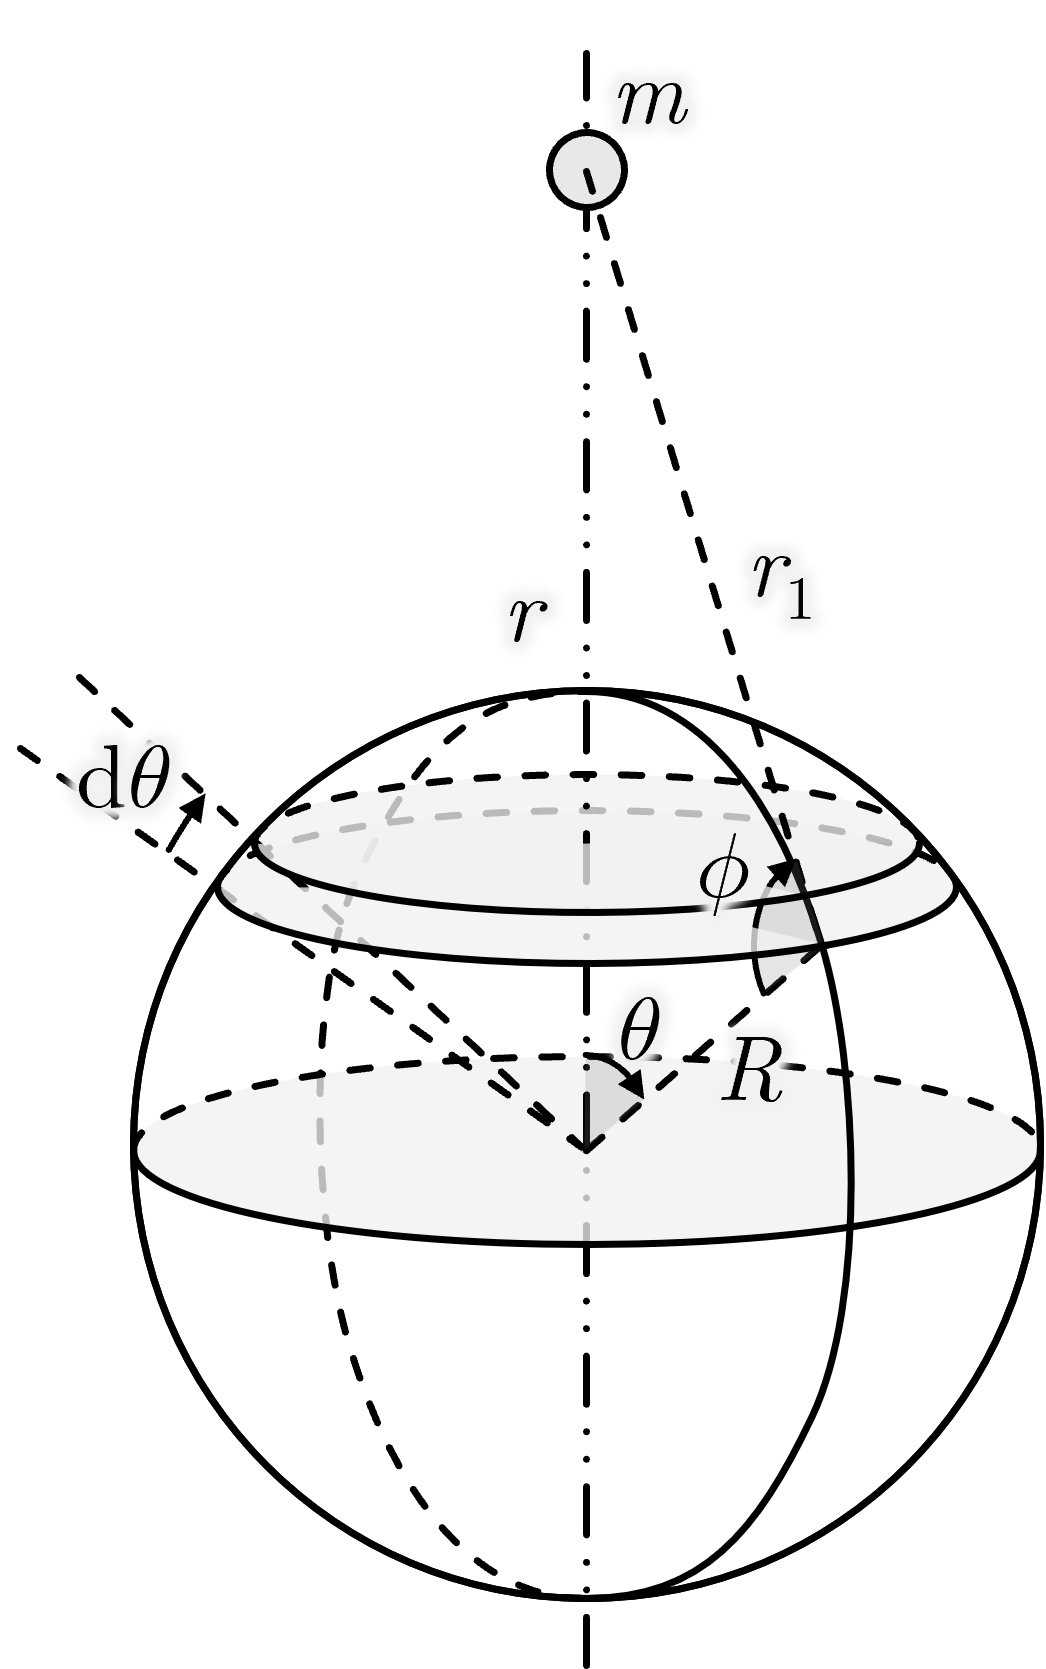
\includegraphics[width=4.07cm]{质点在球外.png}
	\end{wrapfigure}
	\textbf{\wen 质点在球壳外\quad}取球壳上一宽为$R\dif \theta$的环,其质量$M_\text{环} = 2\uppi R\sin\theta \cdot R\dif\theta \cdot \sigma$。这个环产生的引力给质点的引力势能为
	\begin{align*}
		\dif E_{\mathrm{p}\text{壳}} = E_{\mathrm{p}\text{环}} &= \oint -G\dfrac{m \dif M_\text{环}}{r_1}
		= -G\dfrac{m \cdot 2\uppi R\sin\theta \cdot R\dif\theta \cdot \sigma}{r_1} \\[-5pt]
		&= -G\dfrac{m \cdot 2\uppi \sigma R^2 \sin\theta \dif\theta }{r_1}
		\xlongequal{\frac{\sin\phi}{r} = \frac{\sin\theta}{r_1}}
		-G\dfrac{m \cdot 2\uppi \sigma R^2 \sin\phi \dif\theta }{r} \\[-3pt]
		&\xlongequal{\dif r_1 = R\dif \theta \cos\left(\phi-\frac{\uppi}{2}\right)} -G\dfrac{m \cdot 2\uppi \sigma R \dif r_1}{r}
	\end{align*}
	于是,球壳与质点的引力势能为
	\vspace{-1.5em}
	\begin{align*}
		E_{\mathrm{p}\text{壳}} &= \int_\text{球} \dif E_{\mathrm{p}\text{壳}} 
		= \int_{r-R}^{r+R} -G\dfrac{m \cdot 2\uppi \sigma R \dif r_1}{r}
		= -G\dfrac{m \cdot 2\uppi \sigma R \dint_{r-R}^{r+R} \dif r_1}{r} \\[-3pt]
		&= -G\dfrac{m \cdot 2\uppi \sigma R \cdot 2R}{r}
		= -G\dfrac{m \cdot M}{r}
	\end{align*}
	与球壳质量全部集中在球心的情况一样。

	\textbf{\wen 质点在球壳内\quad}上面的分析可完全类似地转到球壳内,即有
	\begin{equation*}
		\dif E_{\mathrm{p}\text{壳}} =
		-G\dfrac{m \cdot 2\uppi \sigma R^2 \sin\phi \dif\theta }{r} 
		\xlongequal{\dif r_1 = R\dif \theta \sin\phi} -G\dfrac{m \cdot 2\uppi \sigma R \dif r_1}{r}
	\end{equation*}

	\begin{wrapfigure}{r}{4.07cm}
		\vspace{-6em}
		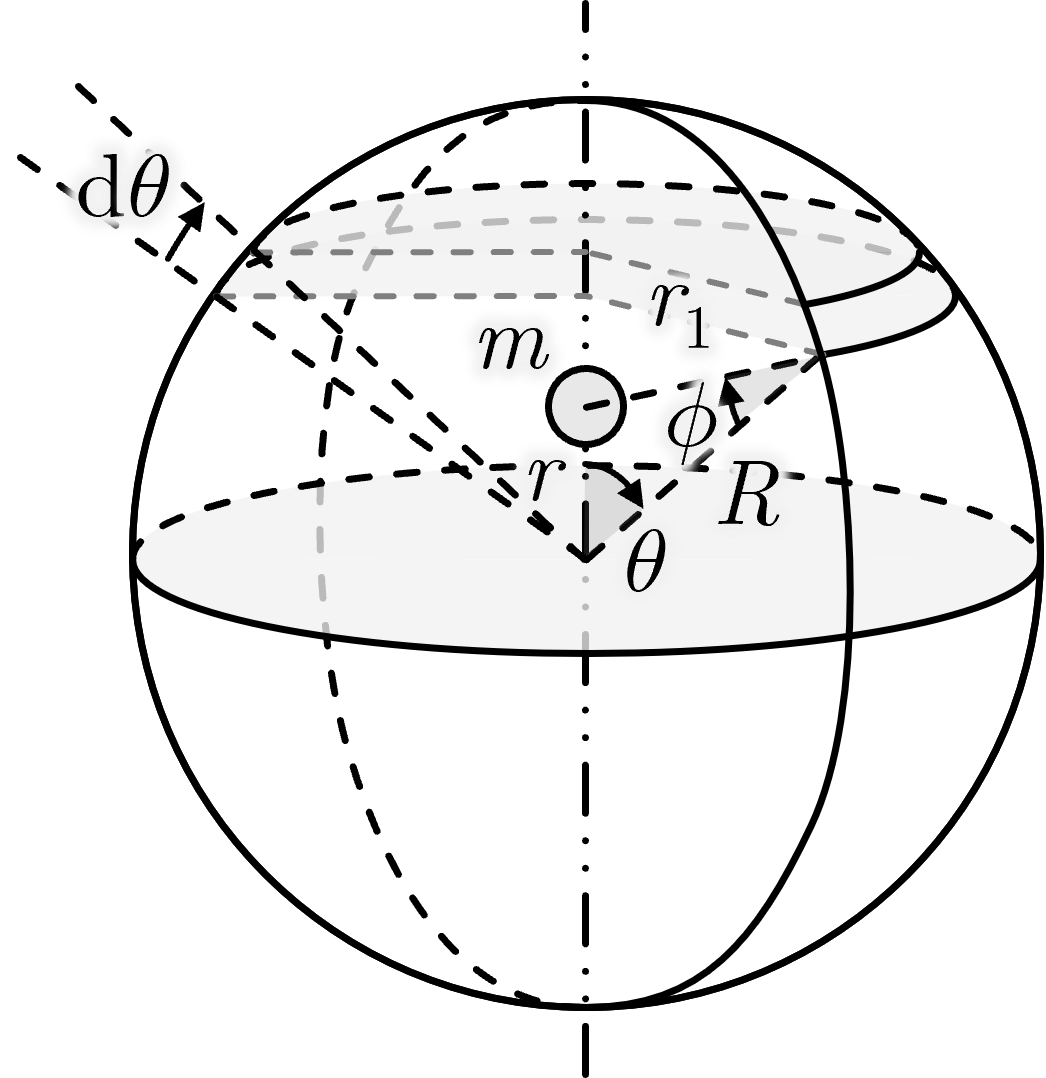
\includegraphics[width=4.07cm]{质点在球内.png}
	\end{wrapfigure}
	于是,球壳与质点的引力势能为
	\begin{align*}
		E_{\mathrm{p}\text{壳}} &= \int_\text{球} \dif E_{\mathrm{p}\text{壳}} 
		= \int_{R-r}^{R+r} -G\dfrac{m \cdot 2\uppi \sigma R \dif r_1}{r}
		= -G\dfrac{m \cdot 2\uppi \sigma R \dint_{R-r}^{R+r} \dif r_1}{r} \\[-3pt]
		&= -G\dfrac{m \cdot 2\uppi \sigma R \cdot 2r}{r}
		= -G\dfrac{m \cdot M}{R}
	\end{align*}

	即球壳内质点在各处的引力势能相等,球壳内任意运动保守力都不做功,故质点在球壳内不受力。
\end{eg}
进一步,对均匀球体内的质点,我们有
\begin{equation*}
	E_\mathrm{p}=-G\frac{m \dfrac{4\uppi r^3}{3} \rho}{r} - Gm \int_r^R \frac{\rho \cdot 4\uppi r^2 \dif r}{r} = \frac12G\frac{Mm}{R}\left(\frac{r^2}{R^2}-3\right)
\end{equation*}
于是可知,$\vr$处质点$m$受到半径$R$的均匀球体$M$的引力为
\begin{equation*}
	\v{F} = -\nabla E_\mathrm{p} = - \dfrac{\dif E_\mathrm{p}}{\dif r} \ur = \begin{cases}[ll]
		-G \dfrac{Mm}{R^3} \vr ,& r<R, \\[7pt]
		-G \dfrac{Mm}{r^2} \ur ,& r>R
	\end{cases}
\end{equation*}
若$m$在此力下做圆周运动,则有 
\begin{equation*}
	F = m\dfrac{v^2}{r} \Longrightarrow v \propto \begin{cases}[ll]
		r,& r<R,\\
		\dfrac{1}{\sqrt{r}},& r>R
	\end{cases}
\end{equation*}
\begin{eg}{开普勒问题}
	\adjline
	前已有$\ddot{\vr}= \left(\ddot{r} - r\dot{\theta}^2\right) \ur + \left(2\dot{r}\dot{\theta} + r\ddot{\theta}\right)\uq$,对受到来自质点$M$引力的物体$m$,我们有
	$$\begin{cases}
		-G\dfrac{Mm}{r^2} = m\left(\ddot{r} - r\dot{\theta}^2\right),\\
		0 \equiv \left(2\dot{r}\dot{\theta} + r\ddot{\theta}\right) = \dfrac{1}{r}\dt\left(r^2\dot{\theta}\right)
	\end{cases} \quad\xLongrightarrow{\text{令}~h \equiv r^2\dot{\theta}}\quad 
	\begin{cases}
		\ddot{r}-\dfrac{h^2}{r^3} + G\dfrac{M}{r} = 0 \\[2pt]
		\dot{\theta}= \dfrac{h}{r^2}
	\end{cases}$$
	解微分方程可得$m$的轨迹,但比较繁琐。

	记$m$的总能量为
	$E = \dfrac{1}{2}m\dot{\vr}^2 - G \dfrac{Mm}{r} = \dfrac{1}{2}m\dot{r}^2 + \dfrac{1}{2}m\left(\dot{\theta}r\right)^2 - G \dfrac{Mm}{r} = \dfrac{1}{2}m\dot{r}^2 + \dfrac{1}{2}m\left(\dfrac{h}{r^2}r\right)^2 - G \dfrac{Mm}{r}$,
	其后两项不与$\dot{r}$有关而与位置$r$有关,记为「等效势能」$V_\mathrm{eff}$。由此解出$\dot{r} = \pm \sqrt{\dfrac{2}{m}(E-V_\mathrm{eff})}$,于是 
	$$ \dfrac{\dif \theta}{\dif r} = \dfrac{\dif \theta}{\dif t}\dfrac{\dif t}{\dif r} = \dfrac{\dot{\theta}}{\dot{r}} = \dfrac{\dfrac{h}{r^2}}{\pm \sqrt{\dfrac{2}{m}(E-V_\mathrm{eff})}} 
	\quad\Longrightarrow\quad 
	\dif \theta = \pm \dfrac{\dfrac{h}{r^2}\dif r}{\sqrt{\dfrac{2}{m}(E-V_\mathrm{eff})}} = \pm \dfrac{\dif\left(\dfrac{1}{r}\right)}{\sqrt{\dfrac{2}{mh^2}(E-V_\mathrm{eff})}} $$

	\begin{wrapfigure}{r}{4.5cm}
		\begin{tikzpicture}
			\draw[-latex] (0,0) node[left]{$M$} to[short, *-] (1.5,0) node[left,below] {$r$};
			\draw[color=bali!50!black, domain=0:360, very thick, smooth, variable=\q] plot(\q:{1/(0.4*cos(\q)+1)}) (-1.8,0) node[left]{$e=0.4$};
			\draw[color=bali!50!black, domain=-120:120, very thick, smooth, variable=\q] plot(\q:{1.4/(cos(\q)+1)}) node[left]{$e=1$};
			\draw[color=bali!50!black, domain=-100:100, very thick, smooth, variable=\q] plot(\q:{2.2/(2*cos(\q)+1)}) node[left]{$e=2$};
		\end{tikzpicture}
		\vspace{2em}
		\begin{tikzpicture}
			\draw[-latex] (0,0) node[left] {$O$}-- (4,0) node[left,below] {$r$};
			\draw[-latex] (0,-1.3) -- (0,2) node[left] {$\epsilon$};
			\draw[color=bali!50!black, domain=0.18:3.6, very thick, smooth, samples=100, variable=\q] plot(\q,{0.2/(\q^2)-0.8/(\q)}) node[below]{$V_\mathrm{eff}$};
			\draw[dashed, color=meihong!50!black, very thick] (0, -0.8) -- (1.2, -0.8) node[anchor=north west]{$E_\mathrm{min}$};
			\draw[dashed, color=meihong!50!black, very thick] (0, -0.5) -- (3, -0.5) node[anchor=north west]{$E<0$};
			\draw[dashed, color=meihong!50!black, very thick] (0, 0) -- (3, 0) node[anchor=south west]{$E=0$};
			\draw[dashed, color=meihong!50!black, very thick] (0, 1) -- (3, 1) node[anchor=south west]{$E>0$};
			%\draw[color=bali!50!black, domain=-120:120, very thick, smooth, variable=\q] plot(\q:{1.4/(cos(\q)+1)}) node[left]{$e=1$};
			%\draw[color=bali!50!black, domain=-100:100, very thick, smooth, variable=\q] plot(\q:{2.2/(2*cos(\q)+1)}) node[left]{$e=2$};
		\end{tikzpicture}
	\end{wrapfigure}

	令$p=\dfrac{h^2}{GM},e=\sqrt{1+\dfrac{2h^2E}{G^2M^2m}}$,则
	\begin{align*}
		\dfrac{2}{mh^2}(E-V_\mathrm{eff}) 
		&= \dfrac{2E}{mh^2} - \dfrac{2}{mh^2}\left(\dfrac{mh^2}{2r^2} - \dfrac{GMm}{r}\right) \\[-3pt]
		&= \dfrac{2E}{mh^2} - \dfrac{1}{r^2} + \dfrac{2GM}{h^2r} \\[-3pt]
		&=	{\color{bali!50!black}\boldsymbol{\dfrac{2E}{mh^2}}}\,
			{\color{meihong!50!black}\boldsymbol{-\, \dfrac{1}{r^2}}}\,
			{\color{meihong!50!black}\boldsymbol{+\, \dfrac{2GM}{h^2r}}}\, 
			{\color{bali!50!black}\boldsymbol{+\, \dfrac{G^2M^2}{h^4}}}\, 
			{\color{meihong!50!black}\boldsymbol{-\, \dfrac{G^2M^2}{h^4}}} \\[-3pt]
		&= {\color{bali!50!black}\boldsymbol{ \dfrac{\dfrac{2Eh^2}{G^2M^2m} + 1}{\dfrac{h^4}{G^2M^2}} }} - {\color{meihong!50!black}\boldsymbol{\left(\dfrac{1}{r} - \dfrac{GM}{h^2}\right)^2}} \\[-3pt]
		&= \dfrac{e^2}{p^2} - \left(\dfrac{1}{r} - \dfrac{1}{p}\right)^2
	\end{align*}

	于是即知$\dif \theta = \pm \dfrac{\dif\left(\dfrac{1}{r}\right)}{\sqrt{\dfrac{e^2}{p^2} - \left(\dfrac{1}{r} - \dfrac{1}{p}\right)^2}} $,积分就有$\theta = \pm  \arcsin\dfrac{p}{e}\left(\dfrac{1}{r}-\dfrac{1}{p}\right) + \chi_1 = \pm  \arccos\dfrac{p}{e}\left(\dfrac{1}{r}-\dfrac{1}{p}\right) + \chi$,即$r= \dfrac{p}{e\cos\left(\theta-\chi\right) + 1}$;不妨取边界条件使得$\chi=0$,则
	$$r= \dfrac{p}{e\cos\theta + 1}$$
	可见相对$M$,$m$的运动轨迹为圆锥曲线,式中$e$即是圆锥曲线的离心率。注意到$e=\sqrt{1+\dfrac{2h^2E}{G^2M^2m}}$中,$e$与1的大小关系取决于$E$与0的大小关系。一方面,从动能与引力势能的关系考虑,则知 
	
	(1)$E>0$,即$\dfrac{1}{2}m\dot{\vr}^2 > G \dfrac{Mm}{r}$时,$e>1$,轨迹为双曲线的一支;
	
	(2)$E=0$,即$\dfrac{1}{2}m\dot{\vr}^2 = G \dfrac{Mm}{r}$时,$e=1$,轨迹为抛物线;

	(3)$E<0$,即$\dfrac{1}{2}m\dot{\vr}^2 < G \dfrac{Mm}{r}$时,$e<1$,轨迹为椭圆。

	另一方面,也可以从$E=\dfrac{1}{2}m\dot{r}^2 + V_\mathrm{eff}$的角度讨论。右图的能量($\epsilon$)—距离($r$)图像中,由于动能项$\dfrac{1}{2}m\dot{r}^2 \ge 0$,能量水平线在$V_\mathrm{eff}$曲线上方的部分就是质点的活动范围。可以看出,当$E<0$时,$m$与$M$之间的距离$r$有限,轨迹呈椭圆形;特别地,$E=E_\mathrm{min}$时$r$有唯一值,轨迹呈圆形。当$E=0$时,$m$恰能运动到无限远处,轨迹为抛物线,当$E>0$时轨迹为双曲线的一支。
\end{eg}

\paragraph{弹性势能}
以弹簧自然长度处为原点,有
\begin{equation*}
	E_\mathrm{p}(x_1) - E_\mathrm{p}(x_2) = W_{x_1\to x_2}
	= \int_{x_1}^{x_2} -kx \dif x
	= -k \cdot \eval{\frac{1}{2}x^2}_{x_1}^{x_2} 
	= \frac{k}{2}\left(x_1^2-x_2^2\right)
\end{equation*}
自然地,取弹簧自然长度处弹性势能为$0$,有$E_\mathrm{p}(x)=\dfrac{1}{2}kx^2$。


\subsubsection{有心力场}
\de[有心力]{
	方向始终指向(背向)固定中心的力,大小仅与到固定中心的距离有关的力,表达为$\v{F}=f(r)\ur$。
}
有心力场是保守力场,势能为$V(r) = \dint_r^{r_0} f(\rho) \dif\rho + V(r_0)$。

质点在有心力场中运动的两个重要特征,一是角动量守恒,运动必在一个平面上,有
$$\v{L} = \vr \cp m\vv = r\ur \cp m(\dot{r} \ur + r\dot{\theta} \uq) = mr^2\dot{\theta}(\ur \cp \uq)$$
二是机械能守恒,即
$$E = \dfrac{1}{2}m\vv^2 + V(r) = \dfrac{1}{2}m(\dot{r}^2+r^2\dot{\theta}^2) + V(r)$$
整理就得到\textbf{研究质点在有心力场中运动的两个基本方程}:
$$\begin{cases}
	mr^2\dot{\theta} = L,\\
	\dfrac{1}{2}m\dot{r}^2 + \dfrac{L^2}{2mr^2} + V(r) = E,
\end{cases} \qq{其中}\begin{cases}
	\v{L} = \vr_0 \cp m\vv_0, \\
	E = \dfrac{1}{2}m\vv_0^2 + V(r_0)
\end{cases}$$
相比牛顿方程,这两个方程降为1阶微分方程,这是利用守恒量的优点。

注意到$\dfrac{1}{2}m\dot{r}^2 + \dfrac{L^2}{2mr^2} + V(r) = E$中,$\dfrac{1}{2}m\dot{r}^2$是\tboba{径向动能},$ \dfrac{L^2}{2mr^2} + V(r)$形式上是一个势能,称为\tboba{等效势能}(有效势能)$V_\mathrm{eff}(r)$。

\subsubsection{理想流体的稳定流动}

若液体密度变化不大而假设是常量,且能忽略粘滞性,则认为液体是\tboba{理想流体}。若流体各处的流动速度不随时间改变,则称流体\tboba{稳定流动}。取出流线管中的一段,其两端横截面积是$A_1,A_2$,由稳定流动的连续性,单位时间内两端进出流体的质量应相等,即$\rho_1 v_1 \dif t A_1 = \rho_2 v_2 \dif t A_2$,即有
$$\rho_1v_1A_1 = \rho_2v_2A_2$$
此为理想流体稳定流动的\textbf{连续性方程}。

即使是静流体中,若存在保守力场,各处压强也不相等。设保守力场的单位质量势能函数为$U$,在静流体中取出一个流元,任建$x$轴,在$x$方向上受力分析,即有
$$p(x) \dif a - p(x+\dif x) \dif a + \rho \dif a\dif x \left(-\dfrac{\partial U }{\partial x}\right) = 0 \quad\Longrightarrow\quad \dfrac{\partial p}{\partial x}+\rho\dfrac{\partial U}{\partial x}=0$$

下面考虑上述单位时间内进出$A_1,A_2$流体的能量变化。某处单位质量流体的能量为$E = \dfrac{1}{2}v^2 + U$,与该处的流速与势能有关。由功能原理,对$A_1,A_2$之间的流体有
$$p_1 \cdot A_1v_1 \dif t - p_2 \cdot A_2v_2 \dif t = \Delta M (E_2-E_1)$$
其中由连续性方程有$\Delta M = \rho_1v_1A_1 \dif t = \rho_2v_2A_2 \dif t$,即得到
$$E_2-E_1 = \dfrac{p_1 \cdot A_1v_1 \dif t}{\Delta M } - \dfrac{p_2 \cdot A_2v_2 \dif t}{\Delta M } = \dfrac{p_1}{\rho_1} - \dfrac{p_2}{\rho_2}$$
于是$E_2+\dfrac{p_2}{\rho_2} = E_1+\dfrac{p_1}{\rho_1} $,即得到了一个恒定量
$$\dfrac{p}{\rho} + \dfrac{1}{2}v^2 + U = \mathrm{Const}$$
此为理想流体稳定流动的\textbf{伯努利方程}。

\subsection{刚体的定轴转动}
\begin{abstract}
	\item[转动惯量] $J_z = \sum\limits_i \Delta m_ir_{i\perp}^2 = \dint_\mathcal{O} r_{\perp}^2 \dif m$。
	\begin{itemize}[leftmargin=3em, labelsep=0.25em, itemindent=0em, itemsep=0pt, parsep=0pt, topsep=0pt, partopsep=0pt]
		\item 常用的转动惯量有均匀圆环对过中心垂直轴$J = mR^2$,均匀圆盘对过中心垂直轴$J = \dfrac{1}{2}mR^2$,均匀杆对过质心垂直轴$J_c = \dfrac{1}{12}ml^2$、对过端点垂直轴$J_A = \dfrac{1}{3}ml^2$;
		\item 同轴叠加性:相对同一转轴,$J=\sum\limits_i J_i$;
		\item 平行轴定理:$J = J_c + Md^2$;
		\item 薄平板刚体正交轴定理:$J_z = J_x + J_y$。
	\end{itemize}

	\item[角动量与力矩的冲量矩] 角动量$\v{L} = J\v{\omega}$,力矩的冲量矩$\v{H} = \dint_{t_1}^{t_2} \v{M} \dif t$,有角动量定理$\v{M} = J\v{\alpha}$。
	
	\item[动能与力矩的功] 转动动能$E_\mathrm{k}=\dfrac{1}{2}J\omega^2$,力矩的功$W = \dint_{\theta_1}^{\theta_2} M \dif\theta$,有动能定理$W = \dfrac{1}{2}J\omega_2^2 - \dfrac{1}{2}J\omega_1^2$。
	
	\item[\hspace{-0.6em}*\hspace{0em}刚体的平面运动] 转轴垂直于平面平移时,运动分解为质心的平动和绕质心的转动,$\v{L} = J_c\v{\omega}_c + \vr_c \cp \v{p}_c$。
\end{abstract}

刚体是一类特殊的质点系,其形状和体积不发生变化。平动时,刚体上所有点运动都相同;因此,刚体质点间的相对运动只能是绕某一轴的转动。由欧拉定理,平动和转动可以描述所有质元(质点)的运动。

刚体质心的平动显然是一个三维问题;刚体转动的旋转轴可以沿三维空间任一方向,其由两个角度来定义, 再加上旋转角,所以也是一个三维问题。因此,\textbf{刚体的运动共有六个自由度}。

刚体的定轴转动只有四个自由度,角速度$\v{\omega}$与角加速度$\v{\alpha}$退化为代数量$\omega$和$\alpha$。

\subsubsection{刚体定轴转动定律}

取旋转轴为$z$轴,由$\v{M}_\text{外} = \dt[\v{L}]$,分解得$M_{\text{外}z} = \dt[L_z]$。而 
$$ L_z = \sum\limits_i L_{iz} = \sum\limits_i \Delta m_iv_ir_{i\perp} = \left(\sum\limits_i \Delta m_ir_{i\perp}^2\right)\omega $$
\de[转动惯量]{
	取旋转轴为$z$轴,刚体各质元与其到$z$轴的距离的平方乘积的和,称为刚体相对$z$轴的\tboba{转动惯量},记为$J_z = \sum\limits_i \Delta m_ir_{i\perp}^2 = \dint_\mathcal{O} r_{\perp}^2 \dif m$。
}
\noindent 则有
\di[刚体定轴转动的角动量公式]{
	刚体相对于转动轴的角动量,等于其相对该轴的转动惯量与角速度的乘积,即$\v{L}=J\v{\omega}$。 
}
\di[刚体定轴转动定律]{
	刚体相对其转动轴所受合外力矩,等于刚体相对该轴的转动惯量与其相对该轴转动的角加速度的乘积,即$\v{M} = J\v{\alpha}$。
}

于是,转动问题求解的第一步就是求出转动惯量。常用的转动惯量有:
\begin{table}[ht!]
	\caption{常用转动惯量公式}
	\begin{center}
		\vspace{-1em}
		\begin{tabular}{p{60pt}<{\centering}p{90pt}<{\centering}p{50pt}<{\centering}|p{60pt}<{\centering}p{90pt}<{\centering}p{50pt}<{\centering}}
			\toprule
			\textbf{刚体} & \textbf{轴的位置} & $\boldsymbol{J}$ & \textbf{刚体} & \textbf{轴的位置} & $\boldsymbol{J}$ \\
			\midrule
			\rule{0pt}{15pt}
			均匀圆环 & 过环心垂直于环面 & $mR^2$ &
			均匀圆盘 & 过盘心垂直于盘面 & $\dfrac{1}{2}mR^2$ \\
			\rule{0pt}{20pt}
			均匀圆筒 & 中心轴 & $mR^2$ &
			均匀圆柱 & 中心轴 & $\dfrac{1}{2}mR^2$ \\
			\rule{0pt}{20pt}
			均匀细杆 & 过杆质心垂直于杆 & $\dfrac{1}{12}ml^2$ &
			均匀细杆 & 过一端点垂直于杆 & $\dfrac{1}{3}ml^2$ \\
			\rule{0pt}{20pt}
			均匀球壳 & 直径 & $\dfrac{2}{3}ml^2$ &
			均匀球体 & 直径 & $\dfrac{2}{5}ml^2$ \\[5pt]
			\bottomrule
		\end{tabular}
		\vspace{-1em}
	\end{center}
\end{table}

转动惯量的计算中,下面一些规律或许有帮助。
\begin{theorem}
	\textbf{同轴叠加性\quad}相对同一转轴,刚体各部分转动惯量$J_i$之和,就是刚体整体的转动惯量$J$,即$J=\sum\limits_i J_i$。
\end{theorem}
\di[平行轴定理]{
	刚体相对任意转轴的转动惯量,等于刚体相对过质心平行轴的转动惯量,加上轴间距的平方与刚体总质量的乘积,即$J = J_c + Md^2$。
}
\begin{proofs}
	\adjline
	在垂直于转轴的平面上取定正交的$\left\{\ux,\uy\right\}$,质元$\Delta m_i$相对转轴的位矢为$\vr_i = x_i\ux + y_i\uy$,质心相对转轴的位矢为$\vr_c = x_c\ux + y_c\uy$,则质元$\Delta m_i$相对转轴的过质心平行轴的位矢为$\vr_i' = x_i'\ux + y_i'\uy$。
	
	考虑$J=\sum\limits_i\Delta m_ir_{i\perp}^2=\sum\limits_i\Delta m_i\left(x_i^2+y_i^2\right)$,其中任一分量上(以$\ux$为例)有$\sum\limits_i\Delta m_ix_i^2 =\sum\limits_i\Delta m_i\left(x_i^{\prime}+x_c\right)^2 =\sum\limits_i\Delta m_ix_i'^{2}+2x_c\sum\limits_i\Delta m_ix_i'+x_c^2\sum\limits_i\Delta m_i$,而相对质心$\sum\limits_i\Delta m_ix_i' = 0$,记$\sum\limits_i\Delta m_i = M$,于是 
	\begin{align*}
		J &= \sum\limits_i\Delta m_i\left(x_i^2+y_i^2\right)
		= \sum\limits_i\Delta m_ix_i'^{2} + Mx_c^2 + \sum\limits_i\Delta m_iy_i'^{2} + My_c^2\\[-5pt]
		&= \sum\limits_i\Delta m_i\left(x_i'^{2} + y_i'^{2}\right) + M\left(x_c^2 + y_c^2\right)
		= J_c + Mr_c^2 \qedhere
	\end{align*}
\end{proofs}
\di[薄平板刚体的正交轴定理]{
	薄平板刚体相对垂直于平板平面转动轴的转动惯量,等于其相对平板平面上过垂足两正交轴的转动惯量之和,记为$J_z = J_x + J_y$。
}
\begin{proofs}
	$J_z =\sum\limits_i\Delta m_ir_{i\perp}^2=\sum\limits_i\Delta m_i\left(x_i^2+y_i^2\right)= J_x + J_y$。
\end{proofs}

\subsubsection{转动的动能与动量}
\di[力矩做功公式]{
	力矩$\v{M}$与力矩作用的物体在力矩作用下的角位移$\Delta\v{\theta}$的点乘,等于力矩在这段角位移上对物体做的功,即$W = \dint_{\theta_\mathrm{i}}^{\theta_\mathrm{f}} \v{M} \cdot \dif\v{\theta}$。
}
\begin{proofs}
	$\Delta W =F_\perp\sin\alpha(r_\perp\Delta\theta)  =F_\perp r_\perp\sin\alpha\Delta\theta  =M\Delta\theta $。
\end{proofs}
\di[刚体定轴转动的动能公式]{
	若刚体相对转轴的转动惯量为$J$,绕转轴转动的角速度为$\v{\omega}$,则刚体转动的动能为$E_\mathrm{k} = \dfrac{1}{2}J\omega^2$。
}
\begin{proofs}
	$\dfrac12J\omega^2=\dfrac12\sum\limits_i\Delta m_ir_{\perp i}^2\omega^2=\dfrac12\sum\limits_i\Delta m_iv_i^2$。
\end{proofs}
由结论~\ref{刚体定轴转动的角动量公式}、\ref{刚体定轴转动定律}~及结论~\ref{力矩做功公式}、\ref{刚体定轴转动的动能公式},分别就有
\begin{theorem}
	\textup{\bf 刚体定轴转动的角动量定理\quad}$\dint_{t_1}^{t_2} \v{M}_{\text{外}z} \dif t = J_z\v{\omega}_2 - J_z\v{\omega}_1$。
\end{theorem}
\vspace{-2em}
\begin{theorem}
	\textup{\bf 刚体定轴转动的功能原理\quad}$W_\text{外}+W_\text{内非} = \Delta\left(\dfrac{1}{2}J\omega^2 + \dfrac{1}{2}mv_c^2 + E_\mathrm{p}\right)$。
\end{theorem}

轴方向确定而平动的情况下,刚体的运动可分解为绕某点(通常取质心)的转动和质心的平动分别求解。

\begin{example}[3]
	棒球运动员击球时存在这样一个击球点,使棒球手击球时手受到的振动最小。这个位置被称为打击甜区。求打击甜区的位置。
\begin{solution}\adjline
	设手握处为参考点$O$,棒的质心位置为$x_C$,击球点的位置为$x$,击球瞬间反弹的球给棒一冲击力$f$,手给棒一约束力$f_0$。列出运动方程,由定轴转动定律	$$fx = J_O\alpha$$
	由质心运动定理 $$f - f_0 = ma_c$$
	又有运动学关系$a_c = \alpha r_c$,则解得$f_0 = \left(1-\dfrac{mx_cx}{J_O}\right)f$。令$f_0=0$,即得打击甜区的位置为$x_\mathrm{h} = \dfrac{J_O}{mx_c}$。
\end{solution}
\end{example}

\Subsubsection{进动}


\newpage
%----------------------------------------------------------
\section{狭义相对论基础}

\subsection{牛顿时空观与伽利略变换}

\subsubsection{力学相对性原理}

牛顿定律对任何惯性系成立,形式都是$\v{F} = m\voa$,而由它推出的动量定理、角动量定理、动能定理在任何惯性系的形式,也都是一样的。\textbf{一切力学规律在不同的惯性系中都有相同的形式},这称为\tboba{力学相对性原理}(或牛顿相对性原理)。

力学相对性原理最早由伽利略提出,即\textbf{通过力学实验无法判定一个惯性系的运动状态}。牛顿相对性原理来源于牛顿的时空观:\textbf{时间和空间都是绝对的,时间和空间的间隔测量不依顿于惯性参考系}。

{\kai 
所谓绝对空间是指长度的量度与参考系无关,绝对时间是指时间的量度和参考系无关。这也就是说,同样两点间的距离或同样的前后两个事件之间的时间间隔,无论在哪个惯性参考系中测量都是一样的。
牛顿曾说:「绝对空间,就其本性而言,与外界任何事物无关,而永远是相同的和不动的。」 还说过:「绝对的、真正的和数学的时间自己流逝着,并由于它的本性而均匀地与任何外界对象无关地流逝着。」在牛顿那里,时间和空间的量度是相互独立的。}

\subsubsection{伽利略变换}

结论~\ref{伽利略变换}~告诉我们,若参考系$S'$相对于参考系$S$平动的速度为$\v{u}$,一质点相对于$S'$的速度为$\vv'$,则该质点相对于$S$的速度为$\vv=\vv'+\v{u}$。更普遍地,有:
\di[时空运动的伽利略变换]{
	对同一事件$\mathcal{E}$,在两个惯性系$S$,$S'$之间有 

	\tbome{时间坐标变换\quad}$t_{S'}(\mathcal{E})=t_{S}(\mathcal{E})$;

	\tbome{空间坐标变换\quad}$\vr_{S'}(\mathcal{E}) = \vr_{S}(\mathcal{E}) - \vr_{S}(S')$;

	\tbome{速度变换\quad}$\vv_{S'}(\mathcal{E}) = \vv_{S}(\mathcal{E}) - \vv_{S}(S')$;

	\tbome{加速度变化\quad}$\voa_{S'}(\mathcal{E}) = \voa_{S}(\mathcal{E})$。
}

此外,牛顿力学强调:力与参考系无关,质量与运动无关。由此,\textbf{牛顿力学规律具有伽利略变换对称性}。

\subsection{光速不变性与洛伦兹变换}

\begin{abstract}
	\item[爱因斯坦狭义相对论的基本假设]
	\begin{itemize}
		\item 相对性原理:一切物理规律在任何惯性系中形式相同。
		\item 光速不变原理:光在真空中的速度与发射体的运动状态无关。
	\end{itemize}
	\item[洛伦兹变换] 坐标轴对应平行地构建两参考系$S,S'$,其中$S'$系相对$S$有平动速度$\v{u} = u\ux$,在$t=t'=0$时刻其原点$O,O'$重合。令$\beta=\dfrac{u }{c }$,$\gamma=\dfrac{1}{\sqrt{1-\beta^2}}=\dfrac{1}{\sqrt{1-\dfrac{u^2}{c^2}}}$,则有:
	\begin{itemize}
		\item 时空坐标的洛伦兹变换:
		$$  x'=\dfrac{x-\beta ct }{\sqrt{1-\beta^2}}=\gamma(x-\beta ct), \qquad
			y'=y, \qquad
			z'=z, \qquad
			t'=\dfrac{t-\dfrac{\beta}{c}x}{\sqrt{1-\beta^2}}=\gamma\left(t-\dfrac{\beta}{c}x\right)
		$$
		\item 时空坐标间隔的洛伦兹变换:
		$$  \Delta x'=\gamma(\Delta x-\beta c\Delta t), \qquad
			\Delta y'=\Delta y, \qquad
			\Delta z'=\Delta z, \qquad
			\Delta t'=\gamma\left(\Delta t-\dfrac{\beta}{c}\Delta x\right)
		$$
		\item 速度的洛伦兹变换:
		$$	v_x'=\dfrac{v_x-u}{1-\dfrac{u}{c^2}v_x}, \qquad 
			v_y'=\dfrac{v_y}{\gamma\left(1-\dfrac{u}{c^2}v_x\right)}, \qquad 
			v_z'=\dfrac{v_z}{\gamma\left(1-\dfrac{u}{c^2}v_x\right)}
		$$
	\end{itemize}
	\item[时空间隔不变性] 设两个事件在参考系$S$下的时空坐标之差为$\{\Delta x,\Delta y,\Delta z,\Delta t\}$,定义长度量$ \Delta s = c^2(\Delta t)^2 -\left[(\Delta x)^2 + (\Delta y)^2 + (\Delta z)^2\right]$,则对任意$S$,$\Delta s$均为同一值,称为这两个事件的时空间隔。
	\item[钟慢效应(固有时间最短)] 运动参考系中的时间流逝变慢,时间间隔比例系数为$\dfrac{1}{\gamma}$。
	\item[尺缩效应(固有长度最长)] 运动的物体长度变短,长度比例系数为$\dfrac{1}{\gamma}$。
\end{abstract}

\subsubsection{狭义相对论的基本假设}

\di[爱因斯坦狭义相对论的基本假设]{
	\tbome{相对性原理\quad}一切物理规律在任何惯性系中形式相同。

	\tbome{光速不变原理\quad}光在真空中的速度与发射体的运动状态无关。
}
在牛顿力学的观念下,时间、长度、质量的标定与测量与参考系无关,而速度与参考系有关。但在狭义相对论下,假定光速不变,则长度、时间、质量将与参考系有关。

在火车上$A'$,$B'$分别放置信号接收器,中点$M$放置光信号发生器,$t=t'=0$时刻$M'$发一光信号。考虑 
\begin{itemize}
	\item 事件A:$A'$接收到闪光;
	\item 事件B:$B'$接收到闪光,
\end{itemize}
则在$S'$系中,A,B在$t'=\dfrac{d }{c}$时刻同时发生,而在$S$系中,事件A先发生。这说明,\textbf{时间间隔是相对的,同时性与惯性系相关,时间随惯性系变化}。

\subsubsection{洛伦兹变换}
\di[时空坐标的洛伦兹变换]{
	坐标轴对应平行地构建两参考系$S,S'$,其中$S'$系相对$S$有平动速度$\v{u} = u\ux$,在$t=t'=0$时刻其原点$O,O'$重合,则两个参考系中的时空坐标$(x,y,z,t)$与$(x',y',z',t')$之间有变换关系
	$$  x'=\dfrac{x-ut }{\sqrt{1-\dfrac{u^2}{c^2}}}, \qquad
		y'=y, \qquad
		z'=z, \qquad
		t'=\dfrac{t-\dfrac{u}{c^2}x}{\sqrt{1-\dfrac{u^2}{c^2}}}
	$$
	令$\beta=\dfrac{u }{c }$,$\gamma=\dfrac{1}{\sqrt{1-\beta^2}}=\dfrac{1}{\sqrt{1-\dfrac{u^2}{c^2}}}$,则
	\vspace{-1.5em}
	$$  x'=\dfrac{x-\beta ct }{\sqrt{1-\beta^2}}=\gamma(x-\beta ct), \qquad
		y'=y, \qquad
		z'=z, \qquad
		t'=\dfrac{t-\dfrac{\beta}{c}x}{\sqrt{1-\beta^2}}=\gamma\left(t-\dfrac{\beta}{c}x\right)
	$$
}
\begin{proofs}[推导]
	\adjline[3]
	在$t=t'=0$时刻其原点$O,O'$重合,此时假定自原点发出闪光,考虑事件P:光传到$P$点,其在两个参考系中的时空坐标分别为$P_S(x,y,z,t)$,$P_{S'}(x',y',z',t')$。
	
	由光速不变原理,$\begin{cases}
		x^2 + y^2 + z^2 = c^2t^2,\\
		x'^2 + y'^2 + z'^2 = c^2t'^2\text{。}
	\end{cases}$由两个参考系的对称性,由反证法易知垂直于参考系相对运动方向上有$y'=y,z'=z$。此时已经可见伽利略变换失效。

	秉持匀速运动物体在所有惯性系都是匀速运动的观念,假设时空坐标$(x,t)$与$(x',t')$之间成线性变换关系,即有$\begin{cases}
		x' = ax + bt, \\ t' = \xi x + \eta t,
	\end{cases}$ 则代入光速不变关系式就有
	$$\begin{cases}
		x^2 + y^2 + z^2 = c^2t^2,\\
		(ax + bt)^2 + y^2 + z^2 = c^2(\xi x + \eta t)^2
	\end{cases} \quad\Longrightarrow\quad \begin{cases}
		ab = c^2\xi\eta,\\
		a^2 - c^2\xi^2 = 1,\\
		c^2\eta^2-b^2 = c^2
	\end{cases}$$
	考虑特殊情况简化计算。令$x'=0$,即对$S'$系中$y'O'z'$平面上的点,其在$S$系中的速度$\dt[x] = u$,于是由$x' = ax + bt$知$\dfrac{b }{a }=-u$;令$x=0$,即对$S$系中$yOz$平面上的点,其在$S'$系中的速度$\dfrac{\dif x'}{\dif t'} = -u$,即有$\dfrac{\dif x'}{\dif t'}=\dfrac{\dif x'}{\dif t}\dfrac{\dif t}{\dif t'} = \dfrac{b}{\eta} = -u$。于是推出$a = \eta$,则$b = c^2\xi = -au$,又由$c^2\eta^2-b^2 = c^2$,解出$a=\dfrac{1}{\sqrt{1-\dfrac{u^2}{c^2}}}$。
\end{proofs}

当$u \ll c$时,$\gamma \to 1$,洛伦兹变换的表达式与伽利略变换一致。

要使变换表达式有意义,则$\beta < 1$,即$u < c$。这说明,\textbf{任何参考系下任何物体的速度都不能超过光速}。

\di[时空坐标间隔的洛伦兹变换]{
	坐标轴对应平行地构建两参考系$S,S'$,其中$S'$系相对$S$有平动速度$\v{u} = u\ux$,在$t=t'=0$时刻其原点$O,O'$重合,则两事件在两个参考系中的时空坐标之差($\{\Delta x,\Delta y,\Delta z,\Delta t\}$与$\{\Delta x',\Delta y',\Delta z',\Delta t'\}$)之间有变换关系
	$$  \Delta x'=\gamma(\Delta x-\beta c\Delta t), \qquad
		\Delta y'=\Delta y, \qquad
		\Delta z'=\Delta z, \qquad
		\Delta t'=\gamma\left(\Delta t-\dfrac{\beta}{c}\Delta x\right)
	$$
}

由此可知,如果两事件在$S$系下同时不同地发生,即$\Delta t = 0$而$\Delta x \neq 0$,则可知$\Delta t' = -\dfrac{\beta\gamma}{c}\Delta x \neq 0$,即它们在$S'$系下不同时发生,在$S'$相对$S$速度所指向一侧的事件先于另一事件。

\zhu[狭义相对论中的时序因果关系]{
	设有两个事件$\mathrm{P}_1,\mathrm{P}_2$,在$S$系中的时空坐标为$P_1(x_1,t_1),P_2(x_2,t_2)$,在$S'$系中的时空坐标为$P_1(x_1',t_1'),P_2(x_2',t_2')$。由洛伦兹变换就有
	$$
	\Delta t'=\gamma\left(\Delta t-\dfrac{\beta}{c}\Delta x\right)=\gamma\Delta t\left(1-\dfrac{u}{c^2}\dfrac{\Delta x}{\Delta t}\right)
	$$
	若$\mathrm{P}_1$是因,$\mathrm{P}_2$是果,则在$S$系中联系二者的\tboqi{信号速度}为$v_s = \dfrac{\Delta x}{\Delta t}$。物体运动的速度和信息传递的速度都不会超过光速,即有$v_s \le c,u \le c$,故$1-\dfrac{u}{c^2}v_s > 0$。则知$\Delta t$与$\Delta t'$同号,两事件在两个参考系中保持时序因果关系。

	若$\mathrm{P}_1,\mathrm{P}_2$相互独立,则对$\dfrac{\Delta x}{\Delta t}$没有限制,可能导致$\Delta t$与$\Delta t'$反号,即出现时序颠倒的情况。
}

\di[时空间隔不变性]{
	坐标轴对应平行地构建两参考系$S,S'$,其中$S'$系相对$S$有平动速度$\v{u} = u\ux$,在$t=t'=0$时刻其原点$O,O'$重合。设有两事件在两个参考系中的时空坐标之差为$\{\Delta x,\Delta y,\Delta z,\Delta t\}$和$\{\Delta x',\Delta y',\Delta z',\Delta t'\}$,则 
	$$
	c^2(\Delta t)^2 -\left[(\Delta x)^2 + (\Delta y)^2 + (\Delta z)^2\right] = c^2(\Delta t')^2 -\left[(\Delta x')^2 + (\Delta y')^2 + (\Delta z')^2\right]
	$$
}
\begin{proofs}
	\adjline
	已知$\Delta y'=\Delta y,\Delta z'=\Delta z$,而又有
	\begin{align*}
		c^2(\Delta t')^2-(\Delta x')^2&=c^2\gamma^2\left(\Delta t-\frac\beta c\Delta x\right)^2-\gamma^2(\Delta x-\beta c\Delta t)^2 \\[-6pt]
		&=\gamma^2(c\Delta t-\beta\Delta x-\Delta x+\beta c\Delta t)(c\Delta t-\beta\Delta x+\Delta x-\beta c\Delta t) \\[-6pt]
		&=\gamma^2(1+\beta)(c\Delta t-\Delta x)(1-\beta)(c\Delta t+\Delta x) \\[-6pt]
		&=\gamma^2(1-\beta^2)\left(c^2(\Delta t)^2-(\Delta x)^2\right)=c^2(\Delta t)^2-(\Delta x)^2 \qedhere
	\end{align*}
\end{proofs}
\de[时空不变量]{
	设两个事件在参考系$S$下的时空坐标之差为$\{\Delta x,\Delta y,\Delta z,\Delta t\}$,则长度量$$ \Delta s = c^2(\Delta t)^2 -\left[(\Delta x)^2 + (\Delta y)^2 + (\Delta z)^2\right]$$ 称为这两个事件的\tboba{时空间隔},也称为\tboba{时空不变量}或\tboba{洛伦兹不变量}。
}

\subsubsection{钟慢效应与尺缩效应}

\paragraph{时间的膨胀}

我们研究在某系$S'$中,同一地点先后发生的两个事件的时间间隔(同一只钟测量),与另一系$S$中,在两个地点的这两个事件的时间间隔(两只钟分别测量)的关系。

\begin{definition}
	在某一参考系中,对两个事件,若它们在同一地点先后发生,它们的时间间隔称为\textbf{固有时},用同一只钟测量;若它们在不同地点先后发生,它们的时间间隔称为\textbf{两地时},用两地两只钟分别测量。
\end{definition}

仍令$S'$系相对$S$有平动速度$\v{u} = u\ux$,考察$S'$中的一只钟,则在$S'$下,两事件发生在同一地点,即$\Delta x' =0$,其时间间隔$\Delta t' = \tau$为这两个事件之间的固有时。在$S$系下,$\Delta x=\gamma\left(\Delta x' +\beta c\Delta t'\right) = \gamma u \tau \neq 0$,其时间间隔$\Delta t = \gamma\left(\Delta t' + \dfrac{\beta}{c}\Delta x'\right) = \gamma \tau$为两地时。由$\gamma > 1$,知$\Delta t > \tau$,即知两个事件之间的所有时间间隔中\textbf{固有时最短}。这个结论也可由时空间隔不变性推出。

由于在两地时对应的参考系看来,固有时对应的参考系在两个事件发生地之间运动,则这个结论也即 
\di[钟慢效应]{
	运动参考系中的时间流逝变慢,时间间隔比例系数为$\dfrac{1}{\gamma}$。
}

\zhu[钟慢效应的相对性]{
	在$S$系中看,$S'$系相对$S$有平动速度$\v{u} = u\ux$,其中发生的事件时间间隔变为$S$系下看到的时间间隔的$\dfrac{1}{\gamma}$;那么由相对性原理,在$S'$系中看,$S$系相对$S$也有平动速度$\v{u}' = -u\ux'$,其中发生的事件时间间隔也应该变为$S'$系下看到的时间间隔的$\dfrac{1}{\gamma}$。这并不矛盾。

	设事件1:$S'$系中A'点与$S$系A点重合,事件2:$S'$系中A'点与$S$系B点重合。以下记号中,带「$'$」号的是$S'$系中的时空参量。
	
	\hang[2](1)从$S$系看来,A、B等地时钟是对准的,在事件1发生时与$S'$系A'时钟同时开始走时。在事件2发生时,若B地时钟走到$\Delta t_1$,则A'时钟走到$\Delta t_1' = \gamma\left(\Delta t_1 - \dfrac{\beta}{c}\cdot u\Delta t_1\right) = \dfrac{1}{\gamma}\Delta t_1$。这就是前面的结论。

	\hang[2](2)从$S'$系看来,$S$系A、B等地时钟不是对准的。例如,在$S$系中我们认为如果在A、B中点处有一个光源发出一瞬闪光,那么在A、B两点处各自收到闪光信号时开始计时,两地时钟就是对准的。但在$S'$系看来则不然,由于$S$系相对$S$有平动速度$\v{u}' = -u\ux'$,则B地钟会先收到闪光,先开始走时,由 Einstein火车模型 可求出其比A地时钟快$t_\mathrm{B,i} = \dfrac{\gamma\beta}{c}x_\mathrm{B}'$。设在事件1发生时$S$系A时钟与$S'$系A'时钟同时开始走时,则事件2发生时有$t_\mathrm{B,f} = \gamma \Delta t_2' = \gamma \dfrac{x_\mathrm{B}'}{c\beta}$。于是B地时钟走过的时间为$\Delta t_2 = t_\mathrm{B,f} - t_\mathrm{B,i} = \dfrac{x_\mathrm{B}'}{c\beta\gamma} = \dfrac{1}{\gamma}\Delta t_2'$。

	于是可见,$S$系看$S'$系中发生的事件时间间隔变为$\dfrac{1}{\gamma}$,$S'$系看$S$系中发生的事件时间间隔也变为$\dfrac{1}{\gamma}$,二者并不矛盾。

	\begin{center}
		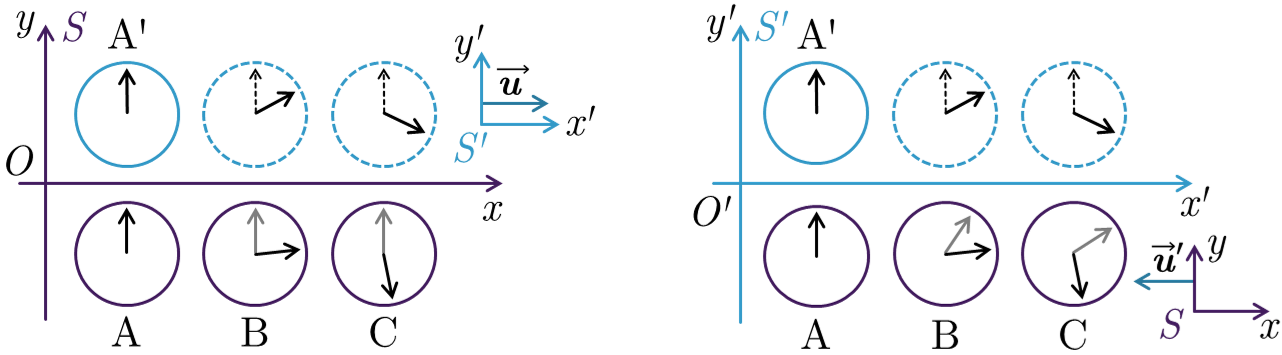
\includegraphics[width=10.86cm]{钟慢效应的相对性.png}
		\captionof{figure}{钟慢效应中同时的相对性}
	\end{center}
}

\paragraph{长度的收缩}

仍令$S'$系相对$S$有平动速度$\v{u} = u\ux$,考察$\ux$方向上的一根直棒的长度。规定长度的测量要求同时测,即测量时间坐标相同时空间坐标的差。

\begin{definition}
	棒静止时测得的它的长,称为该棒的\textbf{固有长度},也称静长或原长,记为$\ell$。
\end{definition}

在$S$中同时测量棒的左右两端,由洛伦兹变换就有$\ell = \gamma\left(l - u\Delta t\right) = \gamma l$。由$\gamma >1$,有$\ell>l$,即知空间两点之间的所有长度中\textbf{固有长度最长}。
\di[尺缩效应]{
	运动的物体长度变短,长度比例系数为$\dfrac{1}{\gamma}$。
}

\begin{eg}{多普勒效应}
	仍令$S'$系相对$S$有平动速度$\v{u} = u\ux$,在$t=t'=0$时刻其原点$O,O'$重合,此时$S$系发出第一个信号并立即被$S'$接收到。之后$t=\tau$时刻$S$系发出第二个信号,在$t'=\tau'$时刻被$S'$接收到。那么,发第二个信号时,光源在$S'$系的位置为$x_s'=\gamma(0-c\beta\tau)=-c\beta\tau\gamma$,在$S'$系的时刻为$t_s'=\gamma\tau$,于是
	$$\tau'=\dfrac{\left|x_s'\right|}{c}+t_s'=(1+\beta)\gamma\tau=\tau\sqrt{\dfrac{1+\beta}{1-\beta}}$$
	若两个信号分别是一列波的两个相邻波峰,则$S$发出的信号频率$\nu$与$S'$收到的信号频率$\nu'$之间满足
	$$\nu' = \nu \sqrt{\dfrac{1-\beta}{1+\beta}}$$
	其中$\beta$符号由相对运动决定。$O,O'$相远离时,$\beta>0$,$\sqrt{\dfrac{1-\beta}{1+\beta}}<1$,有$\nu'<\nu$,即有光谱的红移。
\end{eg}

\subsubsection{相对论速度变换}

坐标轴对应平行地构建两参考系$S,S'$,其中$S'$系相对$S$有平动速度$\v{u} = u\ux$,在$t=t'=0$时刻其原点$O,O'$重合。定义$S,S'$系中$\ux$方向的速度分量$v_x = \dfrac{\dif x}{\dif t}$,$v_x' = \dfrac{\dif x'}{\dif t'}$。由洛伦兹变换有$\begin{cases}
	\dif x'=\gamma(\dif x-c\beta\dif t),\\
	\dif t'=\gamma\left(\dif t-\dfrac{\beta}{c}\dif x\right)
\end{cases}$,两式之比即为
$$v_x'=\dfrac{\dif x'}{\dif t'}=\dfrac{\dif x-c\beta\dif t}{\dif t-\dfrac{\beta}{c}\dif x}=\dfrac{\dfrac{\dif x}{\dif t}-c\beta}{1-\dfrac{\beta}{c}\dfrac{\dif x}{\dif t}}=\dfrac{v_x-c\beta}{1-\dfrac{u}{c^2}v_x}$$
同时还有$\dfrac{\dif t'}{\dif t}=\gamma\left(1-\dfrac{u}{c^2}v_x\right)$,于是有
$$v_y'=\dfrac{\dif y'}{\dif t'}=\dfrac{\dif y}{\dif t}\dfrac{\dif t}{\dif t'}=\dfrac{v_y}{\gamma\left(1-\dfrac{u}{c^2}v_x\right)}, \qquad v_z'=\dfrac{\dif z'}{\dif t'}=\dfrac{\dif z}{\dif t}\dfrac{\dif t}{\dif t'}=\dfrac{v_z}{\gamma\left(1-\dfrac{u}{c^2}v_x\right)}$$

\di[速度的洛伦兹变换]{
	坐标轴对应平行地构建两参考系$S,S'$,其中$S'$系相对$S$有平动速度$\v{u} = u\ux$,在$t=t'=0$时刻其原点$O,O'$重合,则一质点在$S,S'$中的速度$\vv=v_x\ux+v_y\uy+v_z\uz$和$\vv'=v_x'\ux'+v_y'\uy'+v_z'\uz'$之间有变换关系 
	$$v_x'=\dfrac{v_x-c\beta}{1-\dfrac{u}{c^2}v_x}, \qquad 
	v_y'=\dfrac{v_y}{\gamma\left(1-\dfrac{u}{c^2}v_x\right)}, \qquad 
	v_z'=\dfrac{v_z}{\gamma\left(1-\dfrac{u}{c^2}v_x\right)}$$
}

\subsection{相对论下的质量、动量、能量}

\begin{abstract}
	\item[狭义相对论下的质量、动量、动能] 在惯性系$S$中,若有静止质量为$m_0$的质点相对$S$系以速度$\vv$运动,则
	$$	m=\dfrac{m_0}{\sqrt{1-\dfrac{v^2}{c^2}}}=\gamma m_0 \qquad\qquad 
		\v{p}=\dfrac{m_0\vv}{\sqrt{1-\dfrac{v^2}{c^2}}}=\gamma m_0\vv \qquad\qquad
		E_\mathrm{k}=\gamma m_0c^2-m_0c^2
	$$
	\item[狭义相对论运动方程] 在惯性系$S$中,质量为$m$的质点相对$S$系以速度$\vv$运动,其在力$\v{F}$下产生的加速度为
	$$	\voa = \dfrac{\v{F}}{m}-\dfrac{\left(\vv\cdot\v{F}\right)\vv}{mc^2}	$$
	\item[质能关系] 若一运动质点的相对论质量为$m$,则其总能量为$E=mc^2$。
	\item[相对论的动量与能量关系] 设有质点静止质量为$m_0$,动量为$\v{p}$时总能量为$E$,则$E^2 = p^2c^2 + m_0^2c^4$。
	\item[\hspace{-0.6em}*\hspace{0em}动量与能量的洛伦兹变换] 坐标轴对应平行地构建两参考系$S,S'$,其中$S'$系相对$S$有平动速度$\v{u} = u\ux$,则一质点在两个参考系中的动量$\v{p}=p_x\ux+p_y\uy+p_z\uz$与$\v{p}'=p_x'\ux'+p_y'\uy'+p_z'\uz'$、能量$E$与$E'$之间有变换关系
	$$  p_x'=\gamma\left(p_x-\dfrac{\beta}{c}E\right), \qquad
		p_y'=p_y, \qquad
		p_z'=p_z, \qquad
		E'=\gamma\left(E-c\beta p_x\right)
	$$
\end{abstract}

\subsubsection{狭义相对论动力学}

先前提及,动量守恒定律是比牛顿运动定律更基本的规律。下面由洛伦兹变换和动量守恒导出狭义相对论的质量变换。

坐标轴对应平行地构建两参考系$S,S'$,其中$S'$系相对$S$有平动速度$\v{u} = u\ux$,在$t=t'=0$时刻其原点$O,O'$重合。假定在$S'$系中有两个静止质量$m_{1\text{静}}=m_{2\text{静}}=m_0$相同的质点1、2,以相反的速度$\vv_1'=u\ux',\vv_2'=-u\ux'$相向运动。则在$S'$系中,质点1、2的质心静止,即$v'_c=0$。在$S$系中,由洛伦兹变换有$v_c=u$,$v_1=\dfrac{2u}{1+\dfrac{u^2}{c^2}}$,$v_2=0$,则由$S$系下质点系动量表达式$(m_{1\text{动}}+m_{2\text{静}})v_c = m_{1\text{动}}v_1+m_{2\text{静}}v_2$得
$$\dfrac{m_{1\text{动}}}{m_{2\text{静}}}=\dfrac{v_c}{v_1-v_c}=\dfrac{u}{\dfrac{2u}{1+\dfrac{u^2}{c^2}}-u}=\dfrac{1+\dfrac{u^2}{c^2}}{1-\dfrac{u^2}{c^2}} \xlongequal[\text{得}\,\frac{u }{c }=\frac{c }{v_1}-\sqrt{\frac{c^2}{v_1^2}-1}]{\text{解}\,u^2-\frac{2c^2}{v_1}u+c^2=0}\dfrac{1}{\sqrt{1-\dfrac{v_1^2}{c^2}}}$$
即以$v_1$速度运动的质点动质量为$m=\dfrac{m_0}{\sqrt{1-\dfrac{v_1^2}{c^2}}}$。
\di[质量的狭义相对论变换]{
	在惯性系$S$中,若有静止质量为$m_0$的质点相对$S$系以速度$u$运动,则其运动质量为$$m=\dfrac{m_0}{\sqrt{1-\dfrac{u^2}{c^2}}}=\gamma m_0$$
}
\noindent 进而可以回过头定义
\de[狭义相对论动量]{
	考虑相对论效应,在惯性系$S$中,若有静止质量为$m_0$的质点相对$S$系以速度$\vv$运动,则其\tboba{狭义相对论动量}定义为$\v{p}=\dfrac{m_0\vv}{\sqrt{1-\dfrac{v^2}{c^2}}}=\gamma m_0\vv$。
}
仍以动量的变化率为力的定义,则$\v{F}=\dt[\v{p}]=m\voa + \vv\dt[m]$,即$\voa = \dfrac{\v{F}}{m}-\dfrac{\vv }{m}\dt[m]$。而$m=\dfrac{m_0}{\sqrt{1-\dfrac{v^2}{c^2}}}$,则 
$$\dt[m]=-\dfrac{1}{2}\dfrac{m_0}{\left(1-\dfrac{v^2}{c^2}\right)^{\frac{3}{2}}}\cdot\left(-\dfrac{2\vv}{c^2}\right)\cdot\dt[\vv] 
= \dfrac{m}{1-\dfrac{v^2}{c^2}}\cdot\dfrac{\vv}{c^2}\cdot\dt[\vv]
= \dfrac{m\vv}{c^2-v^2}\cdot\voa 
\Longrightarrow \dt[m] = \dfrac{\vv \cdot \v{F}}{c^2}$$
于是有 
\di[狭义相对论运动方程]{
	在惯性系$S$中,质量为$m$的质点相对$S$系以速度$\vv$运动,其在力$\v{F}$下产生的加速度为$$\voa = \dfrac{\v{F}}{m}-\dfrac{\left(\vv\cdot\v{F}\right)\vv}{mc^2}$$
}

\subsubsection{相对论性能量}
设计质点从静止通过力作功使能量增加,能量形式只有动能,则由动能定理有
\begin{equation*}
	\dif W = \v{F}\cdot\dif\vr = \dfrac{\dif \v{p}}{\dif t}\cdot \dif \vr = \vv \cdot \dif\v{p} = \vv \cdot \left(\vv\dif m + m\dif\vv\right)
\end{equation*}
由$m=\dfrac{m_0}{\sqrt{1-\dfrac{v^2}{c^2}}}$,有$m^2(c^2-\vv^2)=m_0^2c^2$,微分即$\dif\bigl(m^2(c^2-\vv^2)\bigr)=2m\dif m(c^2-\vv^2)+m^2(-2\vv\cdot\dif\vv)=0$,即知$c^2\dif m=\vv^2\dif m+m\vv\cdot\dif\vv$,于是
\begin{equation*}
	\dif W = \vv \cdot \vv\dif m + m\vv \cdot \dif\vv = c^2\dif m
	\quad\Longrightarrow\quad E_\mathrm{k}=\int \dif W= \int_{m_0}^m c^2 \dif m = mc^2 - m_0c^2
\end{equation*}
Einstein假设,式中$m_0c^2$是质点除动能以外的所有能量,称之为\tboba{静止能量},而$mc^2$则是运动质点的总能量,即有 
\di[相对论质能关系]{
	若一运动质点的相对论质量为$m$,则其总能量为$E=mc^2$。
}
\noindent 可见,\textbf{相对论质量是能量的量度}。

\begin{theorem}
	\textbf{相对论能量守恒定律\quad}孤立系统中,$E_\mathrm{k} + m_0c^2$为常量,即$\Delta E_\mathrm{k} = -\Delta(m_0c^2)$。
\end{theorem}

上面推导中也得到$m^2(c^2-\vv^2)=m_0^2c^2$,即知有 
\di[相对论的动量与能量关系]{
	设有质点静止质量为$m_0$,动量为$\v{p}$时总能量为$E$,则$E^2 = p^2c^2 + m_0^2c^4$。
}
\begin{eg}{光子的动量与能量}
	光子没有静止质量,$m_0=0$,则$\varepsilon=pc$,而光子的能量$\varepsilon=h\nu$,即知$p=\dfrac{h\nu }{c}=\dfrac{h }{\lambda}$。由$\varepsilon=mc^2$或$p=mc$可定义光子的动质量为$m=\dfrac{h\nu}{c^2}$。
\end{eg}

\Subsubsection{相对论的动量与能量变换}
\kai
下面考虑不同参考系之间动量与能量的变换。由结论~\ref{相对论的动量与能量关系}~,静止质量不变的前提下,$\boldsymbol{\dfrac{E^2}{c^2}-p^2}$\textbf{是洛伦兹不变量}。对应于前述结论~\ref{时空间隔不变性}~及其保证的定义~\ref{时空不变量}~的时空不变量$c^2t^2-r^2$,类比可得对应关系
$$ \frac{E}{c^2} \sim t ,\qquad \v{p} \sim \vr$$
由此,类比结论~\ref{时空坐标的洛伦兹变换}~时空坐标的洛伦兹变换,可得
\di[动量与能量的洛伦兹变换]{
	坐标轴对应平行地构建两参考系$S,S'$,其中$S'$系相对$S$有平动速度$\v{u} = u\ux$,则一质点在两个参考系中的动量$\v{p}=p_x\ux+p_y\uy+p_z\uz$与$\v{p}'=p_x'\ux'+p_y'\uy'+p_z'\uz'$、能量$E$与$E'$之间有变换关系
	$$  p_x'=\gamma\left(p_x-\dfrac{\beta}{c}E\right), \qquad
		p_y'= p_y, \qquad
		p_z'= p_z, \qquad
		E'=\gamma\left(E-c\beta p_x\right)
	$$
}
类似地,由一列电磁波的圆频率$\omega$、波速$c$和波数$\v{k}$满足$\dfrac{\omega}{k}=\dfrac{2\pi\nu}{~\frac{2\pi }{\lambda}~}=c$,有$\dfrac{\omega^2}{c^2}-\v{k}^2=0$也是一个洛伦兹不变量,于是有 
\begin{theorem}
	\textbf{电磁波频率与波数的洛伦兹变换\quad}坐标轴对应平行地构建两参考系$S,S'$,其中$S'$系相对$S$有平动速度$\v{u} = u\ux$,则一列电磁波在两个参考系中的波数$\v{k}=k_x\ux+k_y\uy+k_z\uz$与$\v{k}'=k_x'\ux'+k_y'\uy'+k_z'\uz'$、圆频率$\omega$与$\omega'$之间有变换关系
	$$  k_x'=\gamma\left(k_x-\dfrac{\beta}{c}\omega\right), \qquad
		k_y'= k_y, \qquad
		k_z'= k_z, \qquad
		\omega'=\gamma\left(\omega-c\beta k_x\right)
	$$
\end{theorem}

\begin{example}
	\kai\textbf{资用能\quad}考虑两个粒子$m_1,m_2$的碰撞。不妨在其中一个粒子$m_2$上建立$S$系,其中入射粒子$m_1$的速度为$\vv$,其能量一部分属于质心运动。取两个粒子的质心系$S'$,其为零动量参考系且其中粒子能量$E'$完全用于碰撞,有 
	$$\dfrac{E'^2}{c^2} = \dfrac{E^2}{c^2} - \v{p}^2 = (\gamma m_1+m_2)^2c^2-(\gamma m_1\vv)^2 = (m_1^2+m_2^2+2\gamma m_1m_2)c^2$$
	于是两粒子的内动能为$E^*=E'-(m_1+m_2)c^2=\left(\sqrt{m_1^2+m_2^2+2\gamma m_1m_2}-m_1-m_2\right)c^2$。

	低速时,有$E^* \xlongequal{v \ll c} \dfrac{1}{2}\mu v^2$,与情形~\ref{两体问题之二}~的结论吻合。
\end{example}
\normalfont
\newpage
%----------------------------------------------------------
\section{电磁学:电的规律}

\subsection{真空中的静电场}

\begin{abstract}
	\item[库仑定律] 对真空中两个相距$r$的静止点电荷$q_1$、$q_2$,$q_1$对$q_2$的静电力为
	$\v{F}_{21}=\dfrac{1}{4\pi\varepsilon_0}\dfrac{q_1q_2}{r^2}\ur_{21}$,
	其中\textbf{真空介电常数}$\varepsilon_0 \approx 8.85 \cp 10^{-12} \,\mathrm{C^2/(N\cdot m^2)}$。
	
	\item[常见电荷系的电场强度分布] 记电荷量为$q$,电荷线密度为$\lambda$,电荷面密度为$\sigma$,以下各电荷系产生的场强$\v{E}$与距离$r$的关系为:
	\begin{center}
		\begin{tabular}{lll}
			\toprule
			\multicolumn{2}{l}{\textbf{点电荷电场}}& $\v{E}=\dfrac{q}{4\pi\varepsilon_0r^2}\ur \propto r^{-2}$ \\[7pt]
			\hline
			\textbf{电偶极场} & 中垂线上$r \gg l$处 & $\v{E}= -\dfrac{\v{p}}{4\pi\varepsilon_0r^3} \propto r^{-3}$ \\[7pt]
			& 轴线延长线上($+q$一侧)$r \gg l$处 & $\v{E}= \dfrac{\v{p}}{2\pi\varepsilon_0r^3} \propto r^{-3}$ \\[7pt]
			\multicolumn{3}{l}{其中$\v{p}=q\v{l}_{+-}$为这对电偶极子的电偶极矩,$\v{l}_{+-}$是自$-q$指向$+q$的位矢。}\\[7pt]
			\hline
			\multicolumn{2}{l}{\textbf{均匀带电细棒的电场}} & $E_x = \dfrac{q}{4\pi\varepsilon_0Lx} \sin\theta \Big|_{\theta_\mathrm{i}}^{\theta_\mathrm{f}}$,$E_y = \dfrac{q}{4\pi\varepsilon_0Lx} \cos\theta \Big|_{\theta_\mathrm{f}}^{\theta_\mathrm{i}}$ \\[7pt]
			特别地,& 细棒中垂线上 & $E = E_x = \dfrac{q}{4\pi\varepsilon_0x^2} \dfrac{1}{\sqrt{1+\dfrac{L^2}{4x^2}}}$\\[15pt]
			& \textbf{无限长直线} & $E=\dfrac{q}{2\pi\varepsilon_0Lx}=\dfrac{\lambda}{2\pi\varepsilon_0x} \propto x^{-1}$ \\[7pt]
			\hline
			\multicolumn{2}{l}{\textbf{均匀带电圆环轴线上的电场}} & $E = \dfrac{\sigma x}{2\varepsilon_0} \left(\dfrac{1}{\sqrt{{x}^{2}+{R}_1^{2}}}-\dfrac{1}{\sqrt{{x}^{2}+{R}_2^{2}}}\right)$\\[10pt]
			特别地,& 半径为$R$的\textbf{圆盘} & $E = \dfrac{\sigma}{2\varepsilon_0} \left(1-\dfrac{x}{\sqrt{{x}^{2}+{R}^{2}}}\right)$;\\[7pt]
			& \textbf{无限大平面} & $E = \dfrac{\sigma}{2\varepsilon_0}$为常量\\[7pt]
			\hline
			\multicolumn{2}{l}{\textbf{均匀球壳的电场}} & $E=\begin{cases}[ll]
				0,& r<R_1, \\
				\dfrac{\rho}{3\varepsilon_0}\dfrac{r^3-R_1^3}{r^2},& R_1<r<R_2,\\
				\dfrac{q}{4\pi\varepsilon_0r^2},& r>R_2
			\end{cases}$\\[25pt]
			特别地,& 半径为$R$的\textbf{均匀带电球面} & $E=\begin{cases}[ll]
				0,& r<R, \\
				\dfrac{q}{4\pi\varepsilon_0r^2}=\dfrac{\sigma}{\varepsilon_0}\dfrac{R^2}{r^2},& r>R
			\end{cases}$\\[20pt]
			& 半径为$R$的\textbf{均匀带电球体} & $E=\begin{cases}[ll]
				\dfrac{\rho}{3\varepsilon_0}r,& r<R,\\
				\dfrac{q}{4\pi\varepsilon_0r^2}=\dfrac{\rho R^3}{3\varepsilon_0r^2},& r>R
			\end{cases}$\\[20pt]
			& \textbf{无限大带电体} & $E=\dfrac{\rho}{3\varepsilon_0}r$\\
			\bottomrule
		\end{tabular}
	\end{center}
	% \begin{itemize}[leftmargin=1em]
		% \item \textbf{点电荷电场:}$\v{E}=\dfrac{q}{4\pi\varepsilon_0r^2}\ur \propto r^{-2}$。
		
		% \item \textbf{电偶极场:}中垂线上$r \gg l$处$\v{E}= -\dfrac{\v{p}}{4\pi\varepsilon_0r^3} \propto r^{-3}$,\\
		%      轴线延长线上($+q$一侧)$r \gg l$处$\v{E}= \dfrac{\v{p}}{2\pi\varepsilon_0r^3} \propto r^{-3}$,\\
		% 其中$\v{p}=q\v{l}_{+-}$为这对电偶极子的电偶极矩,$\v{l}_{+-}$是自$-q$指向$+q$的位矢。

		% \item \textbf{均匀带电细棒的电场:}$E_x = \dfrac{q}{4\pi\varepsilon_0Lx} \sin\theta \Big|_{\theta_\mathrm{i}}^{\theta_\mathrm{f}}$,$E_y = \dfrac{q}{4\pi\varepsilon_0Lx} \cos\theta \Big|_{\theta_\mathrm{f}}^{\theta_\mathrm{i}}$。\\
		% 特别地,在细棒中垂线上,$y$向场强抵消,$E = E_x = \dfrac{q}{4\pi\varepsilon_0x^2} \dfrac{1}{\sqrt{1+\dfrac{L^2}{4x^2}}}$;\\
		%    \hskip0.8em$x \ll L$时,成为\textbf{无限长直线},有$E=\dfrac{q}{2\pi\varepsilon_0Lx}=\dfrac{\lambda}{2\pi\varepsilon_0x} \propto x^{-1}$。

		% \item \textbf{均匀带电圆环轴线上的电场:}$E = \dfrac{\sigma x}{2\varepsilon_0} \left(\dfrac{1}{\sqrt{{x}^{2}+{R}_1^{2}}}-\dfrac{1}{\sqrt{{x}^{2}+{R}_2^{2}}}\right)$。\\
		% 特别地,$R_1=0,R_2=R$时,成为半径为$R$的\textbf{圆盘},有$E = \dfrac{\sigma}{2\varepsilon_0} \left(1-\dfrac{x}{\sqrt{{x}^{2}+{R}^{2}}}\right)$;\\
		%    \hskip0.8em$R_1=0,R_2 \to +\infty$时,成为\textbf{无限大平面},有$E = \dfrac{\sigma}{2\varepsilon_0}$为常量。

		% \item \textbf{均匀球壳的电场:}$E=\begin{cases}[ll]
		% 	0,& r<R_1, \\
		% 	\dfrac{\rho}{3\varepsilon_0}\dfrac{r^3-R_1^3}{r^2},& R_1<r<R_2,\\
		% 	\dfrac{q}{4\pi\varepsilon_0r^2},& r>R_2 \text{。}
		% \end{cases}$\\
		% 特别地,$R_1=R_2=R$,成为半径为$R$的\textbf{均匀带电球面},有$E=\begin{cases}[ll]
		% 	0,& r<R, \\
		% 	\dfrac{q}{4\pi\varepsilon_0r^2}=\dfrac{\sigma}{\varepsilon_0}\dfrac{R^2}{r^2},& r>R\text{;}
		% \end{cases}$\\
		%    \hskip0.8em$R_1=0,R_2=R$,成为半径为$R$的\textbf{均匀带电球体},有$E=\begin{cases}[ll]
		% 	\dfrac{\rho}{3\varepsilon_0}r,& r<R,\\
		% 	\dfrac{q}{4\pi\varepsilon_0r^2}=\dfrac{\rho R^3}{3\varepsilon_0r^2},& r>R \text{;}
		% \end{cases}$\\
		%    \hskip0.8em$R_1=0,R_2\to +\infty$,成为\textbf{无限大带电体},有$E=\dfrac{\rho}{3\varepsilon_0}r$。
	% \end{itemize}

	\item[$\v{E}$\,的高斯定理] 在真空中的静电场内,通过任意封闭曲面的电通量等于该封闭面所包围的电荷的电量的代数和的$\dfrac{1}{\varepsilon_0}$,即$\varPhi_\mathrm{e} = \displaystyle \varoiint \v{E} \cdot \dif\v{S} = \dfrac{\sum q_\text{内}}{\varepsilon_0}$。
\end{abstract}

\subsubsection{电荷相互作用与电场的引入}

我们已知,电荷有两种,相同电荷之间有排斥力,不同电荷之间有吸引力;此外,电荷还具有守恒性和相对论不变性。
实验表明,在自然界电荷总是以一个基本单元的整数倍出现。\tboba{电荷基本单元}就是一个质子或电子所带电量的大小,用$e$表示。$e=1.6021766208(98) \cp 10^{-19}\,\text{C}$。

\textbf{真空}中两个\textbf{静止}的\textbf{点电荷}之间的相互作用力可由库仑定律描述:
\di[库仑定律]{
	对真空中两个相距$r$的静止点电荷$q_1$、$q_2$,$q_1$对$q_2$的静电力为
	\begin{equation}
		\v{F}_{21}=k\dfrac{q_1q_2}{r^2}\ur_{21}=\dfrac{1}{4\pi\varepsilon_0}\dfrac{q_1q_2}{r^2}\ur_{21}
	\end{equation}
	\tcblower
	\hang[3]\textbf{式中\quad}%
	$k=\dfrac{1}{4\pi\varepsilon_0}$——\tbome{静电力常量},$k=8.9880\cp10^9\,\mathrm{N \cdot m^2/C^2} \approx 9 \cp 10^9\,\mathrm{N \cdot m^2/C^2}$;\\
	$\varepsilon_0$——\tbome{真空介电常数},$\varepsilon_0 \approx 8.85 \cp 10^{-12} \,\mathrm{C^2/(N\cdot m^2)}$。
}

库仑定律只讨论两个静止的点电荷之间的作用力。若有两个以上静止的点电荷,实验告诉我们,\textbf{两个点电荷之间的作用力并不因第三个点电荷的存在而改变}。为了讨论多个电荷的相互作用,认为电荷的存在在其周围激发出\tboba{电场},电场对放在其内的任何电荷都有作用力,电场力对移动的电荷作功。点电荷之间的静电力,就是一个电荷激发的电场对另一个电荷的电场力。

\de[电场强度]{
	空间中某点处的\tboba{电场强度}定义为
	\begin{equation}
		\v{E}=\dfrac{\v{F}}{q_0}
	\end{equation}
	\tcblower
	\hang[3]\textbf{式中\quad}%
	$q_0$——空间中某点处放置的正试验电荷的电荷量;\\
	$\v{F}$——正试验电荷所受到的电场力。
}

电场强度是空间坐标的函数,它是从「力」的角度来描述电场的一个物理量。

\zhu[近代物理学视角下的电场理论]{
	近代物理学表明,电磁场不仅是研究电荷之间相互作用的简便方法,而是一种客观实在,而且可以脱离电荷和电流存在。电磁场和实物粒子一样就有能量和动量等属性,这在迅速变化的电磁场情形下更为突出地表现出来。
}

\textbf{静电场}是相对观测者静止的电荷产生的电场。

\subsubsection{静止的点电荷的电场及其叠加}

\di[电场的叠加原理]{
	两个点电荷之间的作用力并不因第三个点电荷的存在而改变。
	
	即,设有$N$个静止的点电荷$q_1$、$q_2$、$\cdots$、$q_N$,它们单独存在时的场强分别为$\v{E}_1$、$\v{E}_2$、$\cdots$、$\v{E}_N$,则它们同时存在时的场强为$\v{E}=\sum\limits_{i=1}^N \v{E}_i$。
}

原则上,以点电荷的电场强度公式与场强叠加原理,就可以求得任意点电荷系的场强。

\paragraph{孤立的静止点电荷的电场}

由库仑定律直接得
\begin{equation}
	\v{E}=\dfrac{\v{F}}{q_0}=\dfrac{1}{4\pi\varepsilon_0}\dfrac{qq_0}{r^2}\ur\cdot\dfrac{1}{q_0}=\dfrac{q}{4\pi\varepsilon_0r^2}\ur \propto r^{-2}
\end{equation}
这个电场是以该点电荷为中心球对称的、与$r$平方反比的非均匀场。

\paragraph{电偶极场}

一对靠得很近的等量异号点电荷称为\tboba{电偶极子}。电偶极子在$r \gg l$处($l$为两点电荷间距)产生的电场称为\tboba{电偶极场}。

在电偶极子的中垂线上,
\begin{align}
	\v{E}=\v{E}_++\v{E}_-&=\dfrac{q}{4\pi\varepsilon_0\left( \sqrt{r^2+\left( \frac{l}{2} \right)^2} \right)^2}\left( \ur_+-\ur_- \right)
	\xlongequal{r \gg l} \dfrac{q}{4\pi\varepsilon_0r^2}\left( \frac{\vr_+}{r}-\frac{\ur_-}{r} \right) \nonumber\\[-5pt]
	&= -\dfrac{q\v{l}_{+-}}{4\pi\varepsilon_0r^3}
	= -\dfrac{\v{p}}{4\pi\varepsilon_0r^3} \propto r^{-3}
\end{align}
其中$\v{l}_{+-}$是自$-q$指向$+q$的位矢,$\v{p}=q\v{l}_{+-}$称为这对电偶极子的\tboba{电偶极矩}。在原子分子物理学中,电偶极矩的常用单位为Debye(D,德[拜]),$1 \,\mathrm{D}=1\cp10^{-18} \,\mathrm{e.s.u.cm}= 3.33564 \cp 10^{-30} \,\mathrm{C \cdot m}$。典型的双原子分子的电偶极矩约0到10 D,
如同核双原子分子$\mathrm{N_2}$电偶极矩为0,
而孤立的极性分子NaCl的电偶极矩为9 D。

在电偶极子轴线延长线上(不妨设在$+q$一侧),则有 
\begin{align}
	\v{E}=\v{E}_++\v{E}_-
	&=\dfrac{q}{4\pi\varepsilon_0}\left( \dfrac{1}{(r-\frac{l}{2})^2} - \dfrac{1}{(r+\frac{l}{2})^2}\right) \ur 
	=\dfrac{q}{4\pi\varepsilon_0} \dfrac{(r+\frac{l}{2})^2-(r-\frac{l}{2})^2}{(r-\frac{l}{2})^2(r+\frac{l}{2})^2} \ur \nonumber\\[-3pt]
	&= \dfrac{q}{4\pi\varepsilon_0} \dfrac{2rl}{(r-\frac{l}{2})^2(r+\frac{l}{2})^2} \ur
	\xlongequal{r \gg l}\dfrac{q}{4\pi\varepsilon_0}\dfrac{2lr}{r^4} \ur
	= \dfrac{\v{p}}{2\pi\varepsilon_0r^3} \propto r^{-3}
\end{align}
事实上,可以证明,电偶极场中任意方向上远处($r \gg l$)都有$E \propto r^{-3}$。

\paragraph{均匀带电细棒的电场}

设细棒的长度为$L$,带电量为$q$,记其电荷线密度$\dfrac{q }{L }=\lambda$,则对$\theta$的增量$\dif \theta$,垂直于棒方向上有
\begin{equation*}
	\dif E_x = \dfrac{1}{4\pi\varepsilon_0} \dfrac{\lambda \dif(x \tan \theta)}{\left(\dfrac{x}{\cos\theta}\right)^2} \cos\theta
	= \dfrac{\lambda}{4\pi\varepsilon_0x} \cos^3\theta \dif \tan\theta
	= \dfrac{q}{4\pi\varepsilon_0Lx} \cos\theta \dif \theta
\end{equation*}
从而
\begin{equation*}
	E_x = \int_{\theta_\mathrm{i}}^{\theta_\mathrm{f}} \dfrac{q}{4\pi\varepsilon_0Lx} \cos\theta \dif \theta
	= \dfrac{q}{4\pi\varepsilon_0Lx} \sin\theta \Big|_{\theta_\mathrm{i}}^{\theta_\mathrm{f}}
\end{equation*}
在细棒中垂线上,$y$向场强抵消,又$\sin\theta \Big|_{\theta_\mathrm{i}}^{\theta_\mathrm{f}} = 2\sin\theta_\mathrm{f} = 2\dfrac{\dfrac{L}{2}}{\sqrt{x^2+\left(\dfrac{L}{2}\right)^2}}$,从而
\begin{equation}
	E = E_x = \dfrac{q}{4\pi\varepsilon_0x^2} \dfrac{1}{\sqrt{1+\dfrac{L^2}{4x^2}}}
\end{equation}
\begin{corollary}
	在靠近均匀带电细棒中部的点处,$x \ll L$,有$E=\dfrac{q}{2\pi\varepsilon_0Lx}=\dfrac{\lambda}{2\pi\varepsilon_0x}$,其中$\lambda$是电荷线密度,此时物理上可以将直线看成「无限长」。
\end{corollary}
\begin{corollary}
	在远离棒的位置,$x \gg L$,有$E=\dfrac{q}{4\pi\varepsilon_0x^2}$,此时物理上可以将直线看成一个点电荷。
\end{corollary}

平行于棒方向上,同理有
\begin{equation*}
	\dif E_y = \dfrac{1}{4\pi\varepsilon_0} \dfrac{\lambda \dif(x \tan \theta)}{\left(\dfrac{x}{\cos\theta}\right)^2} \sin\theta
	= \dfrac{\lambda}{4\pi\varepsilon_0x} \sin\theta\cos^2\theta \dif \tan\theta
	= \dfrac{q}{4\pi\varepsilon_0Lx} \sin\theta \dif \theta
\end{equation*}
从而
\begin{equation*}
	E_y = \int_{\theta_\mathrm{i}}^{\theta_\mathrm{f}} \dfrac{q}{4\pi\varepsilon_0Lx} \sin\theta \dif \theta
	= - \dfrac{q}{4\pi\varepsilon_0Lx} \cos\theta \Big|_{\theta_\mathrm{i}}^{\theta_\mathrm{f}}
	= \dfrac{q}{4\pi\varepsilon_0Lx} \cos\theta \Big|_{\theta_\mathrm{f}}^{\theta_\mathrm{i}}
\end{equation*}

\paragraph{均匀带电圆环轴线上的电场}

首先考察细圆环,设其半径为$R$,总带电量为$q$。在轴线上由对称性有
\begin{equation}
	E = E_\parallel = \int \dfrac{\dif q}{4\pi\varepsilon_0r^2}\cos\theta
		= \dfrac{\cos\theta}{4\pi\varepsilon_0r^2}\int \dif q
		= \dfrac{qx}{4\pi\varepsilon_0r^3}
		= \dfrac{qx}{4\pi\varepsilon_0\left(R^2+x^2\right)^{\frac{3}{2}}}
\end{equation}
于是,对内外径分别为$R_1,R_2$的均匀带电圆环,设面电荷密度为$\sigma$,在半径上取微元$\dif r$,即有 
\begin{align}	
	&\dif E = \dfrac{(2\pi r \dif r \sigma)x}{4\pi\varepsilon_0\left(r^2+x^2\right)^{\frac{3}{2}}} 
	= \dfrac{\sigma x r}{2\varepsilon_0\left(r^2+x^2\right)^{\frac{3}{2}}} \dif r \nonumber\\[-5pt]
	&\Longrightarrow\quad
	E = \dfrac{\sigma x }{2\varepsilon_0}\int_{R_1}^{R_2} \dfrac{r}{\left(r^2+x^2\right)^{\frac{3}{2}}} \dif r 
	= \dfrac{\sigma x}{2\varepsilon_0} \left(-\dfrac{1}{\sqrt{{x}^{2}+{r}^{2}}}\right)\bigg|_{R_1}^{R_2} \nonumber\\[-5pt]
	&\qquad\qquad= \dfrac{\sigma x}{2\varepsilon_0} \left(\dfrac{1}{\sqrt{{x}^{2}+{R}_1^{2}}}-\dfrac{1}{\sqrt{{x}^{2}+{R}_2^{2}}}\right)
\end{align}
特别地,对半径为$R$的圆盘,即$R_1=0,R_2=R$,有$E = \dfrac{\sigma}{2\varepsilon_0} \left(1-\dfrac{x}{\sqrt{{x}^{2}+{R}^{2}}}\right)$;进一步,若圆盘面积无限大,即$R_1=0,R_2 \to +\infty$,则有$E = \dfrac{\sigma}{2\varepsilon_0}$为常量,即「无限大」均匀带电平面产生一个均匀电场。


\subsubsection{\(\v{E}\)\,的高斯定理}

\tboba{电场线}是电场力的性质的形象表示。电场线上每点的切线方向就是该点场强的方向,通过某点处垂直于场强方向上的单位面积的电场线条数与该点场强的大小成正比。

电场线起自正电荷或无穷远处(源),止于负电荷或无穷远处(汇),无电荷处不中断。静电场线有头有尾,不是闭合曲线。在没有电荷的地方,两条电场线不能相交。

\de[电通量]{
	通过任一给定面积的电场线条数称为通过该面积的\tboba{电通量},用$\varPhi_\mathrm{e}$表示。
}
在非均匀电场中,通过任一面积$S$的电通量为
$$\varPhi_\mathrm{e} = \iint \v{E} \cdot \dif\v{S}$$
通过任一封闭面$S$的电通量即写成$\varPhi_\mathrm{e} = \displaystyle \varoiint \v{E} \cdot \dif\v{S}$,其中$\dif \v{S} = \dif S \vu*{n}$,$\vu*{n}$为这一面元的单位法向量。对闭合曲面,约定以向外为正方向。

\din[$\v{E}$\,的高斯定理]{
	在真空中的静电场内,通过任意封闭曲面的电通量等于该封闭面所包围的电荷的电量的代数和的$\dfrac{1}{\varepsilon_0}$,即
	\begin{equation}
		\varPhi_\mathrm{e} = \displaystyle \varoiint \v{E} \cdot \dif\v{S} = \dfrac{\sum q_\text{内}}{\varepsilon_0}
	\end{equation}
}
\begin{proofs}
	包围一个孤立点电荷$q$的任意封闭曲面的电通量等于包围该点电荷的球面的电通量$\varPhi_\mathrm{e} = \displaystyle \varoiint \v{E} \cdot \dif\v{S} = \dfrac{q}{4\pi\varepsilon_0r^2}\cdot 4\pi r^2 = \dfrac{q}{\varepsilon_0}$,而通过不包围点电荷$q$的任意封闭曲面的电通量都等于0。
\end{proofs}
注意,高斯定理中的$\v{E}$,是高斯面内、外全部电荷在高斯面上各处的场强,而$\sum q_\text{内}$只是对高斯面内的电荷求和。
\zhu[高斯定理的适用性]{
	虽然高斯定理是在静电场中由库仑定律推出的,但其适用性要比库仑定律更广。

	对静电场,高斯定理和库仑定律等价;对运动电荷,库仑定律不再成立,但高斯定理仍成立。描述任意电场,需要高斯定理加上电场环路定理,分别描述电场的散度和旋度。
}

高斯定理可以用于求静电场的分布。

\begin{example}[3]
	考虑一均匀带电的球层,其内外径分别为$R_1,R_2$,带电量为$q$,求整个空间中电场强度的分布。
\begin{solution}
	\adjline
	记球层的电荷体密度为$\rho = \dfrac{q}{\dfrac{4}{3}\pi\left(R_2^3-R_1^3\right)}$。由对称性,任取一场点 P,可作高斯面S为过P点与带电球层同心的球面,其上的$\v{E}$大小相同,方向处处与面元垂直,于是
	$$	\varoiint_S \v{E} \cdot \dif \v{S} = \varoiint_S E(r) \dif S = 4\pi r^2 E(r) = \dfrac{q_\text{内}}{\varepsilon_0} 
		\quad\Longrightarrow\quad 
		\v{E}=E(r)\ur = \dfrac{q_\text{内}}{4\pi\varepsilon_0r^2}\ur
	$$
	
	(1)$r>R_2$:有$q_\text{内}=q$,有$\v{E}=E(r)\ur = \dfrac{q}{4\pi\varepsilon_0r^2}\ur$,
	即球层外的电场与全部电荷 $q$ 集中在球心的点电荷的场强一样。	

	(2)$R_1 < r < R_2$:可知$q_\text{内}=\dfrac{4\pi \left(r^3-R_1^3\right)}{3}\rho = \dfrac{r^3-R_1^3}{R_2^3-R_1^3}q$,有
	$$\v{E}=E(r)\ur = \dfrac{q}{4\pi\varepsilon_0\left(R_2^3-R_1^3\right)}\dfrac{r^3-R_1^3}{r^2}\ur=\dfrac{\rho}{3\varepsilon_0}\dfrac{r^3-R_1^3}{r^2}\ur$$

	(3)$r<R_1$:$q_\text{内}=0$,则$E=0$,球层内的空腔中没有电场。
\end{solution}

赋值$\begin{cases}
	R_1=R,\\[-3pt] R_2=R,
\end{cases}$~即得半径为$R$的均匀带电球面的电场分布
\begin{equation}
	\v{E} = \begin{cases}[ll]
		\dfrac{q}{4\pi\varepsilon_0r^2}\ur,& r>R,\\
		0,& r<R
	\end{cases}
\end{equation}
赋值$\begin{cases}
	R_1=0,\\[-3pt] R_2=R,
\end{cases}$~即得半径为$R$的均匀带电球体的电场分布
\begin{equation}
	\v{E} = \begin{cases}[ll]
		\dfrac{q}{4\pi\varepsilon_0r^2}\ur,& r>R,\\[7pt]
		\dfrac{qr}{4\pi\varepsilon_0R^3}\ur,& r<R
	\end{cases}
\end{equation}
特别地,赋值$\begin{cases}
	R_1=0,\\[-3pt] R_2\to+\infty,
\end{cases}$~可得无限大三维带电体的电场
\begin{equation}
	\v{E}=\dfrac{\rho}{3\varepsilon_0}\vr
\end{equation}
\end{example}

由此,注意到各个维度的无限大带电体的场强分布满足
\begin{equation*}
	E_\text{0 D} \propto \dfrac{1}{r^2},\qquad
	E_\text{1 D} \propto \dfrac{1}{r},\qquad
	E_\text{2 D} \propto 1,\qquad
	E_\text{3 D} \propto r
\end{equation*}

\zhu[应用高斯定理求电场强度]{
	仅当带电体上电荷分布具有某种对称性时(如板类、柱类、球类),才能用高斯定理求出其产生的电场分布。
	此时,需要\tboqi{根据场强的对称性选择适当的高斯面},满足:
	\begin{itemize}[leftmargin=1em, topsep=0pt]
		\item 高斯面通过场点;
		\item 高斯面各部分或$\v{S} \parallel \v{E}$,或$\v{S} \perp \v{E}$;
		\item 高斯面上待求的场强只有一个值,以便于提出积分号。
	\end{itemize}
}

\subsection{电势与电势能}

\begin{abstract}
	\item[静电场的环路定理] 真空中的静电场内任意环流为0,即$\displaystyle\oint \v{E}\cdot \dif \v{l} = 0$。
	
	环路定理表明了静电场的保守性。

	\item[电势] 取参考点$P_0$处电势为$\phi_0=0$,则静电场中任一点$P$处电势为一个单位正电荷从静电场中$P$点移到$P_0$点的过程中电场力作的功,即
	$ \phi := \phi - \phi_0 = \phi_{PP_0} = \dint_{\widetilde{PP_0} } \v{E} \cdot \dif\v{l} $。

	\item[电势与场强的微分关系] 电场强度等于电势梯度的负值,即$\v{E} = - \nabla \phi$。
	
	\item[电荷(系)的能量] 电荷(系)的能量分以下两部分:
	\begin{itemize}[leftmargin=1em]
		\item 在外电场中的静电势能,定义为将电荷$q$从静电场中$P$点移到参考点$P_0$的过程中电场力作的功,即
		$ W_\text{外} = A_{PP_0} = \dint_{\widetilde{PP_0}} q\v{E} \cdot \dif \v{l} = q \dint_{\widetilde{PP_0}} \v{E} \cdot \dif \v{l} = q \phi $。

		\item 自身静电势能,离散点电荷系的自能为
		$W_\text{自}=\dfrac{1}{2}\sum\limits_i q_i \phi_i$,
		连续点电荷系的自能为
		$W_\text{自}=\dfrac{1}{2}\dint_\mathcal{O} \phi \dif q$。
	\end{itemize}

	\item[静电场的能量密度] 电场能量密度$w_e$与该处电场强度$E$的平方成正比,比例系数为真空介电常数$\varepsilon_0$的一半,即
	$w_e = \dfrac{\varepsilon_0 E^2}{2}$。
\end{abstract}

\subsubsection{静电场的保守性}

\din[\(\v{E}\)的环路定理]{
	在真空中的静电场内,电场强度沿任意闭合路径的线积分(称为静电场的\tbome{环流})为0,即
	\begin{equation}
		\displaystyle\oint \v{E}\cdot \dif \v{l} = 0
	\end{equation}
}
\begin{proofs}
	点电荷的静电场中,从$P_1$处到$P_2$处移动一个试探电荷$q_0$,电场力作功为
	\begin{align*}
		W_{12} = \int_{\widetilde{P_1P_2} } \v{F} \cdot \dif \v{l}
		= q_0 \int_{\vr_1}^{\vr_2} \v{E} \cdot \dif \v{r}
		= q_0 \int_{r_1}^{r_2} E \dif r
		= q_0 \int_{r_1}^{r_2} \dfrac{q}{4\pi \varepsilon_0 r^2} \dif r
		= \dfrac{q_0q}{4\pi\varepsilon_0}\left( \dfrac{1}{r_1} - \dfrac{1}{r_2} \right)
	\end{align*}
	此功与起点、终点的位置有关,与移动路径无关,说明点电荷的静电场是保守力场。由场强叠加原理,任意点电荷系或连续带电体的静电场也是保守力场。

	因此,若电荷$q_0$在静电场中沿一闭合环路移动一圈,设$P_1$、$P_2$是闭合环路上的两点,那么从$P_1 \to P_2$与从$P_2 \to P_1$静电场力的功正好抵消,即沿闭合环路电场力做功为0,于是静电场的环流为0。
\end{proofs}

环路定理是静电场保守性的直接结果。由静电场保守性,说明静电场存在一个势函数。
\de[电势差、电势]{
	在一个单位正电荷从静电场中$P_1$点移到$P_2$点的过程中电场力作的功,定义为$P_1$点到$P_2$点电势的减量,或称为$P_1$点到$P_2$点的\tboba{电势差},记作
	\begin{equation}
		\phi_{12} = \phi_1 - \phi_2 := \dfrac{A_{12}(q)}{q} = \int_{\widetilde{P_1P_2} } \v{E} \cdot \dif\v{l}
	\end{equation}
	取参考点$P_0$处电势为$\phi_0=0$,则静电场中任一点$P$处\tboba{电势}定义为一个单位正电荷从静电场中$P$点移到$P_0$点的过程中电场力作的功,即
	\begin{equation}
		\phi := \phi - \phi_0 = \phi_{PP_0} = \int_{\widetilde{PP_0} } \v{E} \cdot \dif\v{l}
	\end{equation}
}
电场强度是从电场力的角度来描述电场的物理量。电势是从电场力作功的角度来描述电场的物理量。

习惯上,对有限电荷分布,选无穷远处电势$\phi_\infty = 0$,而对无限大电荷分布,需选适当点为电势零点。实践中,常选大地或机壳的公共线为电势零点。

由电场的叠加原理,一系列带电体在空间某点处产生的总电荷为$\phi = \dint_{\widetilde{PP_0}}\textstyle \v{E} \cdot \dif \v{l} = \dint_{\widetilde{PP_0}}\textstyle \left( \sum\limits_i \v{E}_i \right) \cdot \dif \v{l} = \sum\limits_i \dint_{\widetilde{PP_0}}\textstyle \v{E}_i \cdot \dif \v{l} = \sum\limits_i \phi_i$,即有 
\di[电势的叠加原理]{
	一个点电荷在空间中一点处造成的电势并不因其他点电荷的存在而改变。
	
	即,设有$N$个静止的点电荷$q_1$、$q_2$、$\cdots$、$q_N$,它们单独存在时在空间中一点产生的电势分别为$\phi_1$、$\phi_2$、$\cdots$、$\phi_N$,则它们同时存在时在这点产生的电势为$\phi=\sum\limits_{i=1}^N \phi_i$。
}

电场中电势相等的点组成的面称为\tboba{等势面}。等势面是电场的能的性质的一种形象表示。等势面与电场线处处正交,即等势面上每点的法线方向就是该点场强的方向;等势面密处场强大,等势面的电势沿电场线的方向逐渐减小。

设两个靠得很近的等势面上各有一点$P_1$、$P_2$,$P_1$处场强方向如图~\ref{Pic: 电势与场强的微分关系}~所示,则有微元关系$\v{E} \cdot \dif \v{l} = E_\parallel \dif l = - \dif \phi$,或$E_\parallel = - \dfrac{\dif \phi}{\dif l}$,即电势$\phi$在$\dif \v{l}$方向上的变化率的相反数等于场强$\v{E}$在$\dif \v{l}$方向上的分量。显然,当夹角$\langle \v{E},\dif \v{l} \rangle = 0$时,即$\dif \v{l} = \vu*{n}$时,这个分量最大,$\phi$的变化最快,此最大空间变化率称为电势的梯度。
\begin{figure}[ht!]
	\centering
	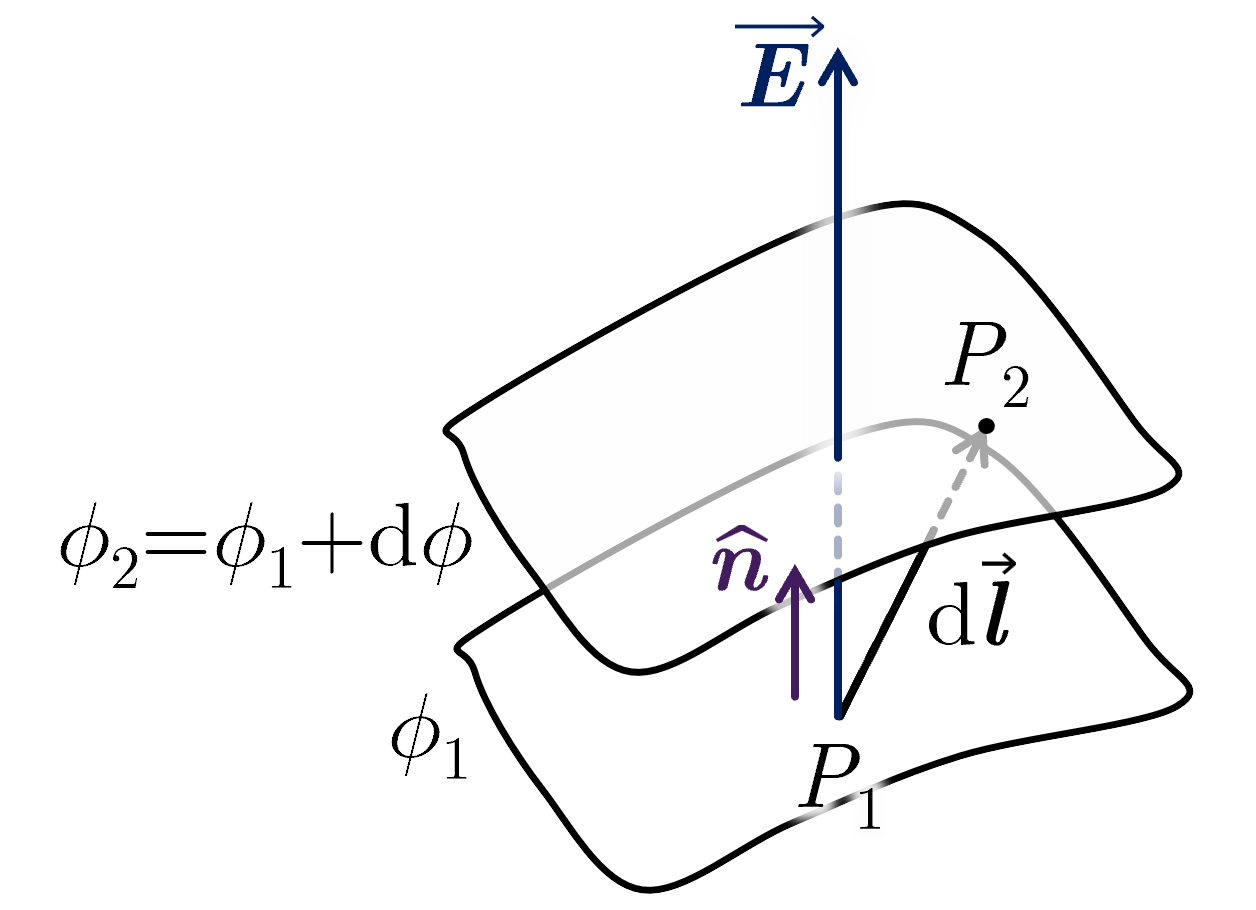
\includegraphics[width=4.9cm]{电势微分.png}
	\caption{电势与场强的微分关系}\label{Pic: 电势与场强的微分关系}
	\vspace{-0.5em}
\end{figure}
\di[电势与电场强度的微分关系]{
	电场强度等于电势梯度的负值,即
	\begin{equation}
		\v{E} = - \v{\nabla} \phi = - \dfrac{\partial \phi}{\partial x}\ux - \dfrac{\partial \phi}{\partial y}\uy - \dfrac{\partial \phi}{\partial z}\uz
	\end{equation}
}

\subsubsection{电荷与电场的能量}

\paragraph{电荷(系)在外电场中的静电势能}

电场力可以对电荷做功,隐含着电荷(系)在外电场中具有能量。

\de[静电(势)能]{
	在电荷$q$从静电场中$P_1$点移到$P_2$点的过程中电场力作的功,定义为电荷$q$从$P_1$点到$P_2$点\tboba{静电势能}的减量。
	
	规定电势零参考点$P_0$处的静电势能为0,则在电荷$q$从静电场中$P$点移到$P_0$点的过程中电场力作的功,定义为电荷$q$在$P$点处的\tboba{静电势能},记作
	\begin{equation}
		W = A_{PP_0} = \int_{\widetilde{PP_0}} q\v{E} \cdot \dif \v{l} = q \int_{\widetilde{PP_0}} \v{E} \cdot \dif \v{l} = q \phi
	\end{equation}
}
静电势能是属于电荷 $q_0$ 和场源所共有的,也叫电荷之间的相互作用能。

\begin{example}[2]
	求一个电偶极矩为$\v{p}$的电偶极子在均匀电场$\v{E}$中的静电势能。
\begin{solution}
	$W=W_++W_-=q(\phi_+-\phi_-)=q\cdot (-\v{E}\cdot \v{l}_{+-})=-\v{p}\cdot \v{E}$。
\end{solution}
\end{example}

\paragraph{电荷系的自身静电势能}

由于同号电荷之间有静电斥力,在带电体形成的过程中,必须有外力克服静电力作功。外力使带电体的各个电荷从分散在无限远处($\phi=0$处)到聚集为电荷系所克服静电力(保守力)所作的功,就成为带电体自身的静电势能。

\de[自能]{
	外力使带电体的各个电荷从分散在无限远处($\phi=0$处)到聚集为电荷系所克服静电力(保守力)所作的功,定义为带电体的\tboba{自身静电势能},简称\tboba{自能}。
}

\di[离散点电荷系的自能公式]{
	离散点电荷系的自能为
	\begin{equation}
		W_\text{自}=\dfrac{1}{2}\sum\limits_i q_i \phi_i
	\end{equation}
	\tcblower
	\hang[3]\textbf{式中\quad}%
	$q_i$——离散点电荷系$i$点电荷的电荷量;\\
	$\phi_i$——离散点电荷系中除$i$点电荷之外其余点电荷在$i$点电荷处的产生的电势。
}
\di[连续点电荷系的自能公式]{
	连续点电荷系的自能为
	\begin{equation}
		W_\text{自}=\dfrac{1}{2}\dint_\mathcal{O} \phi \dif q
	\end{equation}
	\tcblower
	\hang[3]\textbf{式中\quad}%
	$\phi$——连续点电荷系$\mathcal{O}$在其微元$\dif q$处产生的电势。
}

\paragraph{静电场的能量}

对静电场来说,电荷和电场总是同时存在相伴而生的,使我们无法分辨电能是与电荷还是电场相关联。但迅速变化的电场和磁场是以电磁波的形式在空间传播,\textbf{电场可以脱离电荷而传播。}电场储能概念显得非常必要、有用、真实,有必要研究静电能与静电场强度定量关系。

设想一个表面均匀带电的橡皮气球,带电量为$Q$,由于电荷之间的斥力,气球会膨胀。设在某一时刻,气球半径为$R$,静电能量为
$$	W_\text{自} = \dfrac{1}{2}\int_\mathcal{O} \phi \dif q
	= \dfrac{1}{2} Q \cdot \int_{\v{R}}^{\infty} \dfrac{q}{4\pi\varepsilon_0r^2} \ur \cdot \dif \v{r}
	= \dfrac{1}{2} Q \cdot \int_{R}^{+\infty} \dfrac{q}{4\pi\varepsilon_0r^2}  \dif r
	= \dfrac{Q^2}{8 \pi \varepsilon_0 R}
$$
当半径增大$\dif R$时,电荷间的斥力作了正功,此带电气球的静电能量要减少,减少量为
$$	-\dif W = \dfrac{Q^2}{8 \pi \varepsilon_0 R^2} \dif R
$$
半径为$R$的球面内是没有电场的,也没有静电能,半径为$R+\dif R$的薄壳外部的电场并没有变化,只是薄壳层内的电场变为零了,电场消失了,电场的能量也消失了。所以,当半径增大$\dif R$时,气球减少的静电能量就是减少了存储在薄壳层内的电场能量。薄壳层内的电场强度是$\v{E} = \dfrac{q}{4\pi\varepsilon_0R^2} \ur$,即有 
$$	-\dif W = \dfrac{Q^2}{8 \pi \varepsilon_0 R^2} \dif R
	= \dfrac{\varepsilon_0}{2} \cdot \left(\dfrac{Q}{4 \pi\varepsilon_0 R^2}\right)^2 \cdot 4\pi R^2 \dif R 
	= \dfrac{\varepsilon_0 E^2}{2} \dif V
$$
所以单位体积内的电场能量为$w_e = \dfrac{\varepsilon_0 E^2}{2}$。
\de[电场能量密度]{
	单位体积电场所具有的能量,称为\tboba{电场能量}(的体积)\tboba{密度},记作$w_e$。
}
\di[电场能量与电场强度的关系]{
	电场能量密度$w_e$与该处电场强度$E$的平方成正比,比例系数为真空介电常数$\varepsilon_0$的一半,即
	\begin{equation}
		w_e = \dfrac{\varepsilon_0 E^2}{2}
	\end{equation}
}
藉由此,任何一个带电系统的静电场的总能量为$W = \dint_{\R^3} \dfrac{\varepsilon_0E^2}{2}\dif V$。
\zhu[\(\boldsymbol{\dint_{\R^3}\dfrac{\varepsilon_0E^2}{2}\dif{V}}\)(1)与\(\boldsymbol{\dfrac{1}{2}\dint_\mathcal{O}\phi\dif{q}}\)(2)的区别]{
	电场能量密度不可能是负值,因而由式(1)$W = \dint_{\R^3} \dfrac{\varepsilon_0E^2}{2}\dif V$求出的电场能量不可能为负值,但显然式(2)$W = \dfrac{1}{2}\dint_\mathcal{O}\phi\dif{q}$求出的能量可以为负,例如一对电偶极子由(2)求出的能量为负。

	考察由 $+q$ 和$-q$ 组成的电荷系的电场内各点的合电场为$\v{E}=\v{E}_++\v{E}_-$,因而其总电场能量,由式(1)为
	\begin{align*}
		W=\int_{\R^3}\dfrac{\varepsilon_{0}\v{E}^{2}}{2}\dif V
		&=\dfrac{\varepsilon_{0}}{2}\int_{\R^3}(\v{E}_{+}+\v{E}_{-})\cdot(\v{E}_{+}+\v{E}_{-})\dif V\\[-3pt]
		&=\int_{\R^3}\dfrac{\varepsilon_{0}\v{E}_{+}^{2}}{2}\dif V+\int_{\R^3}\dfrac{\varepsilon_{0}\v{E}_{-}^{2}}{2}\dif V+2\int_{\R^3}\dfrac{\varepsilon_{0}\v{E}_{+}\cdot \v{E}_{-}}{2}\dif V
	\end{align*}
	此式最后三项中前两项分别是 $+q$ 和$-q$ 分别孤立存在的电场能量,当然都是正值,第三项即 $+q$ 和$-q$ 的互能(如当$+q$ 和$-q$为点电荷时可证明其值为$-\dfrac{q^2}{4\pi\varepsilon_0 r}$), 它可能为正也可能为负。但因总有$(\v{E}_+-\v{E}_-)^2\ge0$,即$\dfrac{\v{E}_+^2}2+\dfrac{\v{E}_-^2}2\ge \v{E}_+\cdot \v{E}_-$,所以不管互能是正是负,此电荷系的总电场能都会是正的。
}

\subsection{静电场中的导体与绝缘体}

\begin{abstract}
	\item[导体的静电平衡] 特征为:
	\begin{itemize}
		\item 内部各处场强为零,净电荷为零,电势处处相等;
		\item 表面上各处场强与表面垂直,场强大小与面电荷密度成正比,\(\sigma = \varepsilon_0 E\);
		\item 孤立导体表面各处的面电荷密度与各处表面的曲率有关,曲率越大(越尖)的地方,面电荷密度也越大。
	\end{itemize}

	\item[唯一性定理] 在给定的以导体为边界的区域中,若区域内电荷分布确定,且其边界按下列条件之一给定时,区域内的静电场的解必唯一:
	\begin{itemize}[topsep=0pt, leftmargin=1em]
		\item 给定每个导体的电量;
		\item 给定每个导体的电势;
		\item 给定一部分导体的电量和另一部分导体的电势。
	\end{itemize}

	\item[电极化强度] 各向同性电介质内,电极化强度$\v{P}= \varepsilon_0(\varepsilon_\mathrm{r} - 1) \v{E}= \varepsilon_0\chi_e\v{E}$,电极化率$\chi_e = \varepsilon_\mathrm{r} - 1$,表面极化电荷的面密度$\sigma' = \v{P} \cdot \vu*{n}$,内部极化电荷$q' = - \displaystyle \varoiint_S \v{P} \cdot \dif\v{S}$。
	\item[电位移矢量] 各向同性电介质内,电位移矢量$\v{D} = \varepsilon_0\v{E} + \v{P} = \varepsilon_0\v{E} + \varepsilon_0(\varepsilon_\mathrm{r}-1)\v{E} = \varepsilon\v{E}$。
	\item[\(\v{D}\)的高斯定理] 通过任意封闭面的电位移的通量,等于该封闭面所包围的自由电荷的代数和,即
		\(\displaystyle \varoiint_S \v{D} \cdot \dif\v{S} = \textstyle \sum q_\text{0\,内}\)。
	\item[静电场的界面关系] 切向上\(E_{1\uptau}=E_{2\uptau},\dfrac{D_{1\uptau}}{D_{2\uptau}} = \dfrac{\varepsilon_1}{\varepsilon_2}\),法向上\(D_{1\mathrm{n}} = D_{2\mathrm{n}},\dfrac{E_{1\mathrm{n}}}{E_{2\mathrm{n}}} = \dfrac{\varepsilon_2}{\varepsilon_1}\)。
\end{abstract}

\subsubsection{导体的静电平衡与静电屏蔽}

导体在电场中,自由电子受到电场力而运动,这就改变了导体上原来的电荷分布。当导体表面电荷的场和外场相抵消,电荷不再移动,此时称导体在外电场中达到了\tboba{静电平衡}状态。

用场强来表述,静电平衡状态下$\v{E}_\text{内} =\v{0}$,$\v{E}_\text{表} \parallel \dif\v{S}_\text{表}$;用电势来表述,静电平衡状态下的导体是等势体,表面是等势面。静电平衡的导体上的电荷分布具有以下特征:
\begin{itemize}
	\item 导体内部各处净电荷为零,所带电荷只能分布在表面;
	\begin{proofs}
		\adjline
		因静电平衡状态下\(\v{E}_\text{内}=\v{0}\),任作处于导体内部的高斯面,由高斯定律即知其内电荷量\(q_\text{内} = \varepsilon_0 \displaystyle \varoiint_S \v{E} \cdot \dif \v{s} = 0\),故可得出整个导体内部不带电,所以导体所带的电荷只能分布在表面。
	\end{proofs}
	
	\item 导体表面上各处的面电荷密度与当地表面紧邻处的电场强度的大小成正比,比例系数为真空介电常数,即
	\begin{equation}
		\sigma = \varepsilon_0 E \label{equ: 3.10}
	\end{equation}
	\begin{proofs}
		\adjline
		在导体表面紧邻处任取一点\(P\),设该处场强为\(\v{E }\),过\(P\)作一跨表面两侧、底面与临近的导体表面切平面平行的小直柱体,以其表面为高斯面,由高斯定律即知 \(\sigma \dif s = \varepsilon_0 \displaystyle \varoiint_S \v{E} \cdot \dif \v{s} = \varepsilon_0 E \dif s\),即\(\sigma = \varepsilon_0 E\)。
	\end{proofs}
	
	\item 孤立导体表面各处的面电荷密度与各处表面的曲率有关,曲率越大(越尖)的地方,面电荷密度也越大。
	\begin{proofs}
		\adjline
		简化情境,设有两个相距很远的导电球,用细导线连接,求其充电后球面上的电荷分布。
		
		由于相距很远,可以认为导电球的电势$\phi_A = \dfrac{q_A}{4\pi\varepsilon_0R_A} = \phi_B = \dfrac{q_B}{4\pi\varepsilon_0R_B}$,则知$\dfrac{q_A}{R_A} = \dfrac{q_B}{R_B} =: k$。又面电荷密度$\sigma_A=\dfrac{q_A }{4\pi R_A^2}=\dfrac{k}{4\pi R_A}$,$\sigma_B=\dfrac{q_B }{4\pi R_B^2}=\dfrac{k}{4\pi R_B}$,即$\sigma_AR_A = \sigma_BR_B$。即知,虽然大球所带电荷更多,但小球面电荷密度更大。
	\end{proofs}
\end{itemize}

\zhu[有导体存在时静电场的分析与计算]{
	有导体存在时的静电场电荷、场强、电势的分析步骤为:
	
	(1)依据导体的静电平衡条件,设出导体的面电荷,若给出导体总电荷量则写出电荷守恒方程;

	(2)利用高斯定律求电场分布;

	(3)对场强积分求出电势。
}

\begin{example}[1]
	有一块大金属平板,面积为 \(S\),带有总电量 \(Q\),今在其近旁平行地放置第二块大金属平板,此板原来不带电。忽略金属板的边缘效应。
	
	(1)求静电平衡时,金属板上的电荷分布及周围空间的电场分布。
	
	(2)如果把第二块金属板接地,最后情况又如何?

	\begin{solution}\adjline
		(1)由于静电平衡时导体内部无净电荷,所以电荷只能分布在两金属板的表面上。不考虑边缘效应,这些电荷都可当作是均匀分布的。设 4 个表面上的面电荷密度分别为$\sigma_1,\sigma_2,\sigma_3,\sigma_4$,则由电荷守恒可知
		$$\sigma_1+\sigma_2=\dfrac QS,\qquad \sigma_3+\sigma_4=0$$
		由于板间电场与板面垂直,且板内的电场为零,所以选一个两底分别在两个金属板内而侧面垂直于板面的封闭面作为高斯面,由高斯定理即有
		$$\dfrac{(\sigma_2+\sigma_3)S_\text{底}}{\varepsilon_0} = \varoiint \v{E}\cdot\dif\v{s} = 0
		\quad\Longrightarrow\quad 
		\sigma_2+\sigma_3=0$$
		在第二块金属板内任取一点$P$,此处场强$E_P=0$应该是4个带电面的电场的叠加,因而有
		$$E_P=\frac{\sigma_1}{2\varepsilon_0}+\frac{\sigma_2}{2\varepsilon_0}+\frac{\sigma_3}{2\varepsilon_0}-\frac{\sigma_4}{2\varepsilon_0}=0
		\quad\Longrightarrow\quad
		\sigma_1+\sigma_2+\sigma_3-\sigma_4=0$$
		联立求解,可得电荷分布的情况为
		$$\sigma_1=\frac{Q}{2S},\qquad\sigma_2=\frac{Q}{2S},\qquad\sigma_3=-\frac{Q}{2S},\qquad\sigma_4=\frac{Q}{2S}$$
		由此可得电场的分布情况为
		$$E_\text{I}=\dfrac Q{2\varepsilon_{0}S},\text{向左;}\qquad 
		E_\text{II}=\dfrac Q{2\varepsilon_{0}S},\text{向右;}\qquad 
		E_\text{III}=\dfrac Q{2\varepsilon_{0}S},\text{向右}$$

		(2)如果把第二块金属板接地,它就与地这个大导体连成一体,这块金属板右表面上的电荷就会分散到更远的地球表面上而使得这右表面上的电荷实际上消失,因而减少一个电荷守恒式\(\sigma_3+\sigma_4=0\),而多出一个静电平衡条件\(\sigma_4=0\),此时解得
		$$\sigma_1=0,\qquad\sigma_2=\dfrac{Q}{S},\qquad\sigma_3=-\dfrac{Q}{S},\qquad\sigma_4=0$$
		和未接地前相比,电荷分布改变了。这一变化是负电荷通过接地线流入第二块金属板上的结果。这负电荷的电量一方面中和了金属板右表面上的正电荷,另一方面又补充了左表面上的负电荷使其面密度增加一倍。同时第一块板上的电荷全部移到了右表面上。只有这样,才能使两导体内部的场强为零而达到静电平衡状态。这时的电场分布为
		\begin{equation*}
			E_\text{I}=0\text{;}\qquad E_\text{II}=\frac{Q}{\varepsilon_0S},\text{向右;}\qquad E_\text{III}=0 \qedhere
		\end{equation*}
	\end{solution}
\end{example}

利用导体的静电平衡特点,一个接地的封闭金属壳,可以起到壳内外互不影响的屏蔽作用。

\Subsubsection{唯一性定理}

由静电场的基本方程可知,若空间的电荷分布给定,则方程确定,再加上边界条件,空间的电场、能量分布的解确定。唯一性定理讨论的是,有导体存在时解的决定因素。

\di[唯一性定理]{
	在给定的以导体为边界的区域中,若区域内电荷分布确定,且其边界按下列条件之一给定时,区域内的静电场的解必唯一:
	\begin{itemize}[topsep=0pt, leftmargin=1em]
		\item 给定每个导体的电量;
		\item 给定每个导体的电势;
		\item 给定一部分导体的电量和另一部分导体的电势。
	\end{itemize}
}

唯一性定理的意义在于,\textbf{只要找出一种解满足给定的边界条件,它就是该问题的唯一正确解。}

\begin{example}[2]
	点电荷\(q\)放在一个水平的无限大接地金属板的上方\(h\)处,试求:
	
	(1)板上方空间内的电场分布;
	
	(2)板面上的感生电荷分布。

	\begin{solution}
		所讨论的区域是无限大平板上方空间,其边界条件为\(\phi_\text{板} = \phi_\infty = 0\)。设想在导体表面的正下方\(h\)处放另一与上方电荷异号等量的点电荷\(-q\),然后把金属板撤去,得到一对电偶极子的电场。已知在这样的电场中,两电荷连线的垂直平分面(原来金属板表面位置)上的电势也等于零,即这一对电荷的电场的上半部的边界条件和金属板存在时完全一样。由唯一性定理,板上方空间内的电场分布与电偶极子垂直平分面一侧的电场分布完全一致。

		由点电荷电场的叠加可得,板上方任一点$P$处的电场为
		$$\v{E}(\vr)=\frac{q}{4\pi\varepsilon_0 \|\vr-\v{h}\|^3}(\vr-\v{h})-\frac{q}{4\pi\varepsilon_0 \|\vr+\v{h}\|^3}(\vr+\v{h})$$
		式中,$\vr$表示从电荷$q$在平板上的投影点到$P$点的径矢,\(\v{h}\)表示该投影点到电荷$q$的径矢。由此,对于平板上任一点$P_0$,则
		$$\v{E}_0(r)=\frac{q \cdot (-2\v{h})}{4\pi\varepsilon_0(r^2+h^2)^{\frac32}}=-\frac{q\v{h}}{2\pi\varepsilon_0(r^2+h^2)^{\frac32}}$$
		由式~(\ref{equ: 3.10}),\(\sigma(r) = \varepsilon_0 E_0(r) = -\dfrac{qh}{2\pi(r^2+h^2)^{\frac32}}\)。
	\end{solution}
\end{example}

\zhu[电像法]{
	电像法的基本思想是在所求域外放置适当的电像,等效导体边界上未知的感应电荷对域内电场的影响。电像法可以大幅简化问题,但可解决的问题有限。
}

\subsubsection{电介质的极化}

实验表明,在两带电平行板之间插入电介质后,电压变小。插入前后电压的比值,定义为电介质的\tboba{相对介电常数},用$\varepsilon_\mathrm{r}$表示。由电压变为原来的$\dfrac{1}{\varepsilon_\mathrm{r}}$,知场强将变为原来的$\dfrac{1}{\varepsilon_\mathrm{r}}$。

电介质这类物质中,没有自由电子,不导电,也称为绝缘体,其又可分为极性和非极性两类。
\begin{itemize}
	\item 分子中的正电荷等效中心与负电荷等效中心重合的称为\textbf{非极性分子}(如H$_2$、CH$_4$、CO$_2$)。非极性分子在电场中,正负电荷中心会被拉开一段距离,产生感应电偶极矩,这称为\tboba{位移极化}。
	\item 分子中的正电荷等效中心与负电荷等效中心不重合的称为\textbf{极性分子}(如HCl、H$_2$O)。极性分子在电场中,固有电偶极矩会转向电场的方向,这称为\tboba{取向极化}。
\end{itemize}
总之,不管哪种电介质,极化机制虽然不同,放到电场中都有极化现象,都会出现\tboba{极化电荷}(也叫\tboba{面束缚电荷}),正是这些极化电荷的电场削弱了电介质中的电场。

\de[电极化强度]{
	电介质单位体积内分子的电偶极矩的矢量和,定义为电介质的\tboba{电极化强度},记作$\v{P}$,即\begin{equation}
		\v{P}= \dfrac{\sum\limits_i \v{p}_i}{\Delta V}
	\end{equation}
	\tcblower
	\hang[3]\textbf{式中\quad}%
	$\Delta V$——宏观上很小、微观上很大的体积元;\\
	$\v{p}_i$——体积元$\Delta V$中的分子的电偶极矩。
}
电极化强度的单位是$\mathrm{C/m^2}$,即量纲上$[\v{P}] = [\sigma]$。电极化强度反映了介质被极化的程度,即分子电偶极矩排列的有序程度。电极化强度是空间的点函数。

实验表明,$\v{E}$不太强时,各向同性电介质内有$\v{P} \propto \v{E}$,即$\v{P}$总是与$\v{E}$平行,且$\v{P}= \varepsilon_0(\varepsilon_\mathrm{r} - 1) \v{E}$。
定义$\chi_e = \varepsilon_\mathrm{r} - 1$为\textbf{电极化率},则
\begin{equation}
	\v{P}= \varepsilon_0\chi_e\v{E}
\end{equation}

极化电荷是介质极化的结果。下面考察极化强度和极化电荷之间关系。在极化的介质内任意作一闭合面$S$,那么$S$ 把位于$S$ 附近的电介质分子分为两部分,
一部分在$ S $内 , 一部分在$ S $外,其中只有电偶极矩穿过$S$ 的分子对
$S$内外的极化电荷才有贡献(或者说被$S$截为两段的偶极子才对极化电荷有贡献)。

在$S$上取面元$\dif S$,在$\dif S$附近薄层内认为介质均匀极化,电极化强度为$\v{P}$。在$\dif S$两侧对称作平行于$\dif S$的两个面元$\dif S_1$,$\dif S_2$ ,面沿$\v{P}$的方向间距为电偶极子正负电荷的距离$l$。只有被$\dif S$截断的偶极子才对面$S$内电荷有贡献,所以有
$$	|\dif q'| = \big|qnl \cos\langle\dif\v{S},\v{P}\rangle \cdot \dif S\big|
	= \big|P \cdot \dif S \cos\langle\dif\v{S},\v{P}\rangle\big|
	= \big|\v{P} \cdot \dif\v{S}\big|
$$
其中$n$为介质分子数密度。极化电荷的正负取决于$\theta$,$\theta < 90^\circ$时面内计划电荷为负,于是可得小面元$\dif S$附近分子对面内极化电荷的贡献为
\begin{equation*}
	\dif q' = - \v{P} \cdot \dif\v{S} = - P_\mathrm{n} \dif S
\end{equation*}

\begin{circum}
	
\textbf{极化面电荷\quad}由$\sigma'=\dfrac{\dif q'}{\dif S}$,即知
\di[电介质表面电极化强度和极化电荷面密度的关系]{
	在极化的介质表面(外侧),极化电荷的面密度
	\begin{equation}
		\sigma' = \v{P} \cdot \vu*{n}
	\end{equation}
	\tcblower
	\hang[3]\textbf{其中\quad}%
	$\v{P}$——极化的介质表面该处的电极化强度;\\
	$\vu*{n}$——极化的介质表面该处的外法线方向向量。
}

\end{circum}
\begin{example}[1]
	在插入介质的平行板电容器中证明上面理论的自洽性。
\begin{proofs}
	\adjline
	板间电场由两板上的自由电荷$\pm\sigma_0$和电解质表面的束缚电荷$\pm\sigma'$共同产生,前者单独产生的场强为$E_0 = \dfrac{\sigma_0}{\varepsilon_0}$,后者单独产生的场强为$E' = \dfrac{\sigma'}{\varepsilon_0}$,二者方向相反。由场强叠加原理,即有 
	\begin{equation*}
		E = E_0 - E' = \dfrac{\sigma_0}{\varepsilon_0} - \dfrac{\sigma'}{\varepsilon_0}
		\xlongequal{\v{P}=\varepsilon_0(\varepsilon_\mathrm{r}-1)\v{E}}
		\dfrac{\sigma_0}{\varepsilon_0} - \dfrac{\varepsilon_0(\varepsilon_\mathrm{r}-1)E}{\varepsilon_0}
		\quad\Longrightarrow\quad E = \dfrac{\sigma_0}{\varepsilon_0\varepsilon_\mathrm{r}} = \dfrac{E_0}{\varepsilon_\mathrm{r}} \qedhere
	\end{equation*}
\end{proofs}
\noindent 上面过程中,$\varepsilon:= \varepsilon_0\varepsilon_\mathrm{r}$称为\textbf{绝对介电常数}。
\end{example}

\begin{circum}
	
\textbf{极化体电荷\quad}由上面直接有

\di[电极化强度和极化电荷的关系]{
	在极化的介质内任意一闭合面$S$所围的体积内,极化电荷
	\begin{equation}
		q' = - \varoiint_S \v{P} \cdot \dif\v{S}
	\end{equation}
	\tcblower
	\textbf{其中\quad}%
	$\v{P}$——面元$\dif S$附近薄层中的电极化强度。
}
进而,在静电场中的各向同性均匀电介质内,无自由电荷处,必无极化体电荷。

\end{circum}

当外电场很强时,电介质的正负电中心有可能进一步被拉开,变成可以自由移动的电荷,电介质的绝缘性能被破坏而变成了导体了,这称为电介质\textbf{击穿}。电介质能承受的最大电场强度称为该电介质的\textbf{击穿场强},或\textbf{介电强度}。

\subsubsection{$\v{D}$\,的高斯定理}

有电介质时,设空间中存在带电体$q_0$,极化电介质产生了$q'$的极化电荷,则高斯定理表述为$\displaystyle \varoiint_S \v{E} \cdot \dif\v{S} = \dfrac{1}{\varepsilon_0}\textstyle\left( \sum q_\text{0\,内} + \sum q_\text{内}' \right)$。
设法替换掉$q_\text{内}'$,由$\sum q_\text{内}' = \displaystyle -\varoiint_S \v{P} \cdot \dif\v{S}$,得
$$	\varoiint_S \v{E} \cdot \dif\v{S} 
	= \dfrac{\sum q_\text{0\,内}}{\varepsilon_0}-\dfrac{1}{\varepsilon_0}\varoiint_S \v{P} \cdot \dif\v{S} 
	\quad\Longrightarrow\quad 
	\varoiint_S \left( \varepsilon_0\v{E} + \v{P} \right) \cdot \dif\v{S} = \sum q_\text{0\,内}
$$
\de[电位移矢量]{
	空间中某点处的\tboba{电位移矢量}定义为
	\begin{equation}
		\v{D} = \varepsilon_0\v{E} + \v{P}
	\end{equation}
}

$\v{E}$不太强时,我们有$\v{D} = \varepsilon_0\v{E} + \varepsilon_0(\varepsilon_\mathrm{r}-1)\v{E} = \varepsilon\v{E}$。

\din[$\v{D}$的高斯定理,label=D的高斯定理]{
	通过任意封闭面的电位移的通量,等于该封闭面所包围的自由电荷的代数和,即\begin{equation}
		\varoiint_S \v{D} \cdot \dif\v{S} = \sum q_\text{0\,内}
	\end{equation}
}

$\v{D}$的高斯定理比真空中的$\v{E}$的高斯定理更普遍。当没有电介质时,即$\v{P} \equiv \v{0}$,就过渡到真空中的高斯定律了。

\subsubsection{静电场的界面关系}

在介质分界面上,作一扁筒式封闭面为高斯面\(\varSigma\),面积为\(\Dif S\)的两底面分别在两介质内并平行于界面,则由\(\v{D}\)的高斯定律可得
\begin{align*}
	\varoiint_{\varSigma} \v{D} \cdot \dif \v{s} &= \v{D}_1 \cdot \Dif S\vu*{n} + \v{D}_2 \cdot \Dif S (-\vu*{n}) \\[-10pt] 
	&= \bigl(\v{D}_1 \cdot \vu*{n} - \v{D}_2 \cdot \vu*{n}\bigr) \Dif S
	= (D_{1\mathrm{n}}-D_{2\mathrm{n}}) \Dif S = \sigma_0 \Dif S 
	\quad\Longrightarrow\quad D_{1\mathrm{n}}-D_{2\mathrm{n}} = \sigma_0
\end{align*}
在交界面无自由电荷的情形下,即有 
\begin{equation}
	D_{1\mathrm{n}} = D_{2\mathrm{n}},\qquad 
	\dfrac{E_{1\mathrm{n}}}{E_{2\mathrm{n}}} = \dfrac{\varepsilon_2}{\varepsilon_1}
\end{equation}
类似地,在介质分界面上作一窄条矩形环路\(\varGamma\),长度为\(\Dif L\)的两长边分别在两介质内并平行于界面,则由环路定理可得
\begin{align*}
	\oint_\varGamma \v{E} \cdot \dif \v{l} 
	&= \v{E}_1 \cdot \Dif L \vu*{\tau} + \v{E}_2 \cdot \Dif L (-\vu*{\tau}) \\[-10pt] 
	&= \bigl(\v{E}_1 \cdot \vu*{\tau} - \v{E}_2 \cdot \vu*{\tau}\bigr) \Dif L
	= (E_{1\uptau}-E_{2\uptau}) \Dif L = 0 
	\quad\Longrightarrow\quad E_{1\uptau}-E_{2\uptau} = 0
\end{align*}
即 
\begin{equation}
	E_{1\uptau}=E_{2\uptau},\qquad 
	\dfrac{D_{1\uptau}}{D_{2\uptau}} = \dfrac{\varepsilon_1}{\varepsilon_2}
\end{equation}

\subsection{稳恒电流}

\begin{abstract}
	\item[电流的描述] 单位时间内流过某一确定横截面的电量称为\textbf{电流强度},即\(I = \dt[q]\);空间中一点处的电流用\textbf{电流密度}矢量描述,记作\(\v{J}\),其大小等于单位时间通过单位垂直面积的电荷量,方向与正电荷定向运动的方向相同,即\(\v{J}=\dfrac{\dif I}{\dif S_\perp}\vu*{n}_+\)。
	\item[电流连续性方程] 对任一闭合面,电流密度的通量满足\(\displaystyle \varoiint_S \v{J} \cdot \dif\v{S} = - \dt[Q_\text{内}]\)。
	\item[欧姆定律的微分形式] 导体中电场强度为\(\v{E}\)处电流密度为\(\v{J} = \sigma \v{E}\),其中\(\sigma\)是电导率。
	\item[焦耳定律的微分形式] 导体中电场强度为\(\v{E}\)处转化处热能为\(p = \sigma E^2\),其中\(\sigma\)是电导率。
	\item[电动势] 电源内部单位正电荷从负极运动到正极的过程中,非静电力所作的功称为\textbf{电动势},即 
		\(\mathscr{E}=\dfrac{A_\text{非}(q_0)}{q_0}=\displaystyle \oint_{(-)}^{(+)} \v{E}_\text{非} \cdot \dif \v{l}\)。
\end{abstract}

\subsubsection{稳恒电流与稳恒电场}

\de[电流强度]{
	单位时间内流过某一确定横截面的电量称为\tboba{电流强度},简称\tboba{电流},记为$I$,即\begin{equation}
		I = \dt[q]
	\end{equation}
}
对细导线用电流强度的概念就够了。对大块导体,还需电流密度的概念来进一步描写电流的分布。
\de[电流密度]{
	空间中一点处的电流用\tboba{电流密度}矢量描述,记作\(\v{J}\),其大小等于单位时间通过单位垂直面积的电荷量,方向与正电荷定向运动的方向相同,即\begin{equation}
		\v{J}=\dfrac{\dif I}{\dif S_\perp}\vu*{n}_+
	\end{equation}
}
由此即$\dif I = \v{J} \cdot \dif\v{S}$,于是$I = \dint_S \v{J} \cdot \dif\v{S}$,即电流强度是「电流密度的通量」。

\di[电流连续性方程]{
	对任一闭合面,电流密度的通量满足
	\begin{equation}
		\begin{aligned}
			&\text{\tbome{积分形式\quad}} \varoiint_S \v{J} \cdot \dif\v{S} = - \dt[Q_\text{内}] \\
			&\text{\tbome{微分形式\quad}} \nabla \cdot \v{J} + \dfrac{\partial\rho}{\partial t} = 0
		\end{aligned}
	\end{equation}
	\tcblower
	\hang[3]\textbf{其中\quad}%
	$Q_\text{内}$——闭合面包围的电荷;\\
	$\rho$——闭合面中的电荷平均体密度。
}

由可自由运动的电荷产生的电流称为\tboba{传导电流}。依载流子的运动,传导电流密度为$\v{J}_\mathrm{c}=nq\langle\v{u}\rangle$。

恒定电流下导体内各处电流密度不随时间变化,于是有
$$\varoiint_S \v{J} \cdot \dif\v{S} = 0 \quad\text{或}\quad \nabla \cdot \v{J} = 0$$
稳恒电流的电流线必定闭合。
\begin{theorem}
	\textup{\textbf{节点电流方程(基尔霍夫第一定律)}\quad}在稳恒电路中,对任一闭合面,$\sum\limits_i I_{i,\textup{in}}=\sum\limits_i I_{i,\textup{ex}}$。若规定流出该闭合面的电流为正,流入电流为负,则$\sum\limits_i I_i =0$。
\end{theorem}
对于通有稳恒电流的电路,导体内存在稳恒电场,稳恒电场由不随时间改变的电荷分布产生。可以证明,电荷只分布在导体表面和两种导体的界面。\textbf{稳恒电场也满足环路定理。}
\begin{theorem}
	\textup{\textbf{回路电压方程(基尔霍夫第二定律)}\quad}在稳恒电路中,沿任何闭合电路一周,其电势降落的代数和等于零。
\end{theorem}

\subsubsection{欧姆定律与焦耳定律}

由欧姆定律,$U_{ab}=I_{ab}R_{ab}$,其中电势差$U_{ab}=\phi_a-\phi_b$,比例系数$R=\rho\cdot\dfrac{L }{S}$称为\tboba{电阻},与导体的\tboba{电阻率}~$\rho$和形状有关。电阻$R$和电阻率$\rho$的倒数分别称为\tboba{电导}~$G$和\tboba{电导率}~$\sigma$。

将欧姆定律用于大块导体中的一小段,有
\begin{equation}
	\phi - (\phi + \dif \phi) = \v{J} \cdot \dif \v{S} \cdot \rho\dfrac{\dif l}{\dif S} = \v{J} \cdot \vu*{n}_+ \cdot \rho\dif l \qq{$\Longrightarrow$} \v{J} = - \dfrac{1}{\rho} \dfrac{\dif \phi}{\dif l}\vu*{n}_+ = \sigma \v{E}
\end{equation}
这就是\tbome{欧姆定律的微分形式}。

下面由电流的经典微观图象证明上面的式子。对导体中载流子两次碰撞之间的运动,$\vv_i = \vv_{oi} + \dfrac{q\v{E}}{m}t_i$,取统计学平均,热运动$\langle \vv_{0i} \rangle = \v{0}$,则定向漂移速度$ \langle \v{u} \rangle = \dfrac{q\v{E}}{m} \langle t_i \rangle = \dfrac{q\v{E}}{m}\tau$。于是 
$$\v{J}_\mathrm{c}=nq\langle\v{u}\rangle = \dfrac{nq^2\tau}{m}\v{E} =: \sigma \v{E}$$

\begin{example}[3]
	已知大地的电阻率为$\rho$,求半球形接地器(半径为$a$)的接地电阻和跨步电压。
\begin{solution}
	\adjline
	将地分为一层层薄半球壳,任取一层,其半径为$r$,厚为$\dif r$,其电阻为$\dif R_\text{阻} = \rho \dfrac{\dif r}{2\pi r^2}$。于是积分得
	$$R_\text{阻}=\int_a^{+\infty} \rho\dfrac{\dif r}{2\pi r^2}=\dfrac{\rho}{2\pi a}$$
	地中$r$半径上的电流密度为$J = \dfrac{I }{2\pi r^2} = \sigma E$,即$E = \dfrac{I }{2\pi r^2\sigma}$。于是,从距半球中心$b$处向外跨步$c$的跨步电压为
	$$V_\text{跨} = \int_b^{b+c} \dfrac{I }{2\pi r^2\sigma} \dif r = \dfrac{c}{b(b+c)}\dfrac{\rho I}{2\pi}$$
	结合两式,$V_\text{跨} = \dfrac{ac}{b(b+c)}\dfrac{\rho I}{2\pi a} = \dfrac{ac}{b(b+c)} I R_\text{阻} = \dfrac{ac}{b(b+c)} V_\text{输}$。
\end{solution}
\end{example}

由上面的微观解释还可知,一次碰撞后定向运动的能量变成离子的热能的量为
$$\left\langle \dfrac{1}{2}m\v{u}^2 \right\rangle = \dfrac{q^2\v{E}^2}{2m} \left\langle t^2 \right\rangle \xlongequal{\left\langle t^2 \right\rangle = 2 \left\langle t \right\rangle ^2 = 2\tau^2} \dfrac{q^2E^2\tau^2}{m} $$
于是单位时间内导体单位体积内,电能转换为热能的量为$p=\dfrac{n}{\tau}\left\langle \dfrac{1}{2}m\v{u}^2 \right\rangle = \dfrac{nq^2E^2\tau}{m} = \sigma E^2$,
这就是\tbome{焦耳定律的微分形式}。

\subsubsection{电动势}

\de[电动势]{
	在电源内部,单位正电荷从负极到正极的过程中,非静电力所作的功称为\tboba{电动势},记作$\mathscr{E}$,即 
	\begin{equation}
		\mathscr{E}=\dfrac{A_\text{非}(q_0)}{q_0}
	\end{equation}
}
常常把非静电力的作用看成是一种非静电场的作用,以单位正电荷所受到的非静电力$\v{E}_\text{非}$表示非静电场的强度。在电源内部,电荷$q$从负极到正极运动的过程中,非静电力作的功$A_\text{非} = q\dint_{(-)}^{(+)} \v{E}_\text{非} \cdot \dif \v{l}$,即$\mathscr{E}=\dint_{(-)}^{(+)} \v{E}_\text{非} \cdot \dif \v{l}$。由在回路中其他位置没有非静电场,也可对整个回路写出$\mathscr{E}=\displaystyle \oint_{(-)}^{(+)} \v{E}_\text{非} \cdot \dif \v{l}$

由恒定条件和高斯定理知,均匀材质的导线上的电荷只能分布在导线的表面。维持恒定电流的恒定电场,就是由电源正负极上的电荷和导线表面上(或两种材料交界面处)的电荷产生的。当导线的布线形状发生改变时,导线表面上的电荷分布将立刻自动地跟着调整,使导线内的恒定电场仍指向电流流动的方向。电场的传播以光速进行,所以很快。

\begin{eg}{接触电动势和温差电}
	两种不同的金属接触时会出现电势差,这个电势差称为\textbf{接触电动势}。接触电动势的产生有以下原因:
	\begin{itemize}
		\item \textbf{逸出功不同}:金属表面有一层电子气,即有一个约$10^{-10}\,\mathrm{m}$厚的电偶层。电子要真正脱离金属,就必须克服金属表面层这阻碍电子逃逸的电场力作功,这个功$A$称为\textbf{逸出功},其与电偶层的电势差$\phi^*$之间的关系为$A=e\phi^*$。两种金属接触时,若逸出电势$\phi^*_1 < \phi^*_2$,则金属1中电子更易出来,2中的电子将多于金属1中的电子,这是产生接触电动势的原因之一。
		
		\item \textbf{自由电子数密度不同}:若金属1、金属2中的电子数密度$n_1>n_2$,则会出现电子气的扩散,这是产生接触电势差的原因之二。
	\end{itemize}
	总的接触电动势等于开路端电压,即为
	\begin{equation}
		\mathscr{E}=\phi_{12}=\phi^*_2-\phi^*_1 + \dfrac{kT}{e}\ln\dfrac{n_1}{n_2}
	\end{equation}
	把两种金属接成闭合回路,若两个接点A、B处的温度相同,则接点A、B处电动势 抵消,电路中无电动势。若两个接点A、B处的温度不同,则电路中有
	电动势,也有电流。这一对金属即称为\textbf{热电偶},在两个接点温度不同时所产生的接触电动势的差值称为\textbf{温差电动势},也即是热电偶对外显现的电动势,其与两个接点的温差有关。
\end{eg}

\section{电磁学:磁的规律}

\subsection{磁场与磁力的规律}
\begin{abstract}
	\item[磁感应强度] 有三种等价的定义方式:
	\begin{itemize}
		\item \textbf{\run 从运动电荷受力定义}\quad 空间某点的\textbf{磁感应强度},数值上等于单位电荷以单位速率通过该点所受的最大洛伦兹力,方向由这个最大磁力及其对应速度以右手定则确定,即\(\v{F} = q\vv \cp \v{B}\)。
	
		\item \textbf{\run 从电流元受力定义}\quad 空间某点的\textbf{磁感应强度},数值上等于单位电流元在该处所受的最大安培力,方向由这个最大磁力及其对应电流元方向以右手定则确定,即\(\dif\v{F} = I\dif\v{l} \cp \v{B}\)。
	
		\item \textbf{\run 从磁矩受力矩定义}\quad 空间某点的\textbf{磁感应强度},数值上等于单位磁矩(单位电流、单位面积)在该处所受的最大力矩,方向由这个最大力矩及其对应磁矩以右手定则确定,即\(\v{M} = I\v{S} \cp \v{B} = \v{m} \cp \v{B}\)。
	\end{itemize}
	
	\item[\(\v{B}\)的高斯定理] 在任何磁场内,通过任意封闭曲面的磁通量恒等于0,即
		\(\varPhi = \displaystyle \varoiint \v{B} \cdot \dif\v{S} = 0\)。

	\item[Biot-Savart定律] 电流元$I\dif \v{l}$在相对于其$\vr$处产生的磁场为
		\(\dif \v{B} = \dfrac{\mu_0 I\dif\v{l} \cp \ur}{4\pi r^2} = \dfrac{\mu_0}{4\pi}\dfrac{I\dif\v{l}\sin\left\langle I\dif\v{l},\vr \right\rangle}{r^2}\)。

	\item[常见载流路径的磁感应强度分布] 记电流强度为\(I\),以下各载流路径产生的场强\(\v{E}\)和距离\(d\)的关系为:
	\begin{center}
		\begin{tabular}{lll}
			\toprule
			\multicolumn{2}{l}{\textbf{长直电流的磁场}} & $B = \dfrac{\mu_0I}{4\pi d}\left( \cos\theta_1 - \cos\theta_2 \right)$ \\[7pt]
			特别地,& 无限长直电流 & \(B=\dfrac{\mu_0I}{2\pi d}\) \\[7pt]
			& 无限半长直电流 & \(B=\dfrac{\mu_0I}{4\pi d}\) \\[7pt]
			\hline
			\multicolumn{2}{l}{\textbf{圆电流轴线上的磁场}} & $B = B_{\parallel} = \dfrac{\mu_{0}IR^{2}}{2(R^2+d^2)^\frac{3}{2}}$ \\[7pt]
			特别地,& 圆电流中心处 & \(B=\dfrac{\mu_0I }{2R }\) \\[7pt]
			\hline
			\multicolumn{2}{l}{\textbf{磁偶极场}} & \(\v{B} = \dfrac{\mu_0 I\v{S}}{2\pi d^3} = \dfrac{\mu_0 \v{m}}{2\pi d^3}\) \\[7pt]
			\hline
			\multicolumn{2}{l}{\textbf{长直螺线管内轴线上的磁场}} & \(B = \dfrac{\mu_{0}nI }{2} (\cos\beta_2 - \cos\beta_1)\) \\[7pt]
			特别地,& 无限长直螺线管内任一点处 & \(B=\mu_0nI\) \\[7pt]
			& 无限半长直螺线管端部圆心 & \(B=\dfrac{\mu_{0}nI }{2}\) \\[7pt]
			\hline
			\multicolumn{2}{l}{\textbf{无限长圆柱面电流的磁场}} & \(B = \dfrac{\mu_0}{2\pi r}I_\text{内} = \begin{cases}[ll]
				\dfrac{\mu_0I}{2\pi r},& r>R,\\
				0,& 0<r<R
			\end{cases}\) \\[7pt]
			\bottomrule
		\end{tabular}

	\end{center}
	\item[\(\v{B}\)的环路定理] 在恒定电流的磁场中,磁感强度$\v{B}$沿任何闭合路径$L$的线积分(环量)等于路径$L$所环绕的电流强度的代数和的$\mu_0$倍,即
		\(\displaystyle \oint_L \v{B}\cdot\dif\v{l} = \mu_0 \textstyle\sum I_\text{内}\)。
	\item[霍尔效应] 金属窄条沿磁场方向厚度为\(b \),沿第三方向宽度为\(h\),则霍尔电压\(U_\text{H}=vBh=\dfrac{BI}{nbq}\xlongequal{K_\mathrm{H}:=\frac{1}{nq}}K_\mathrm{H}\dfrac{BI}{b}\)。
\end{abstract}
\subsubsection{磁场的规律}

\de[磁感应强度]{
	\hang[1]\tboba{\run 从运动电荷受力定义}\quad 空间某点的\tboba{磁感应强度},数值上等于单位电荷以单位速率通过该点所受的最大洛伦兹力,方向由这个最大磁力及其对应速度以右手定则确定。
	
	\hang[1]\tboba{\run 从电流元受力定义}\quad 空间某点的\tboba{磁感应强度},数值上等于单位电流元在该处所受的最大安培力,方向由这个最大磁力及其对应电流元方向以右手定则确定。

	\hang[1]\tboba{\run 从磁矩受力矩定义}\quad 空间某点的\tboba{磁感应强度},数值上等于单位磁矩(单位电流、单位面积)在该处所受的最大力矩,方向由这个最大力矩及其对应磁矩以右手定则确定。
}
磁感应强度$\v{B}$在SI制中的单位是特斯拉(T),$\mathrm{1\,T = 1 \, \dfrac{N}{C\cdot m/s}}$。在磁学中经常还使用另一种单位制,即高斯制,在高斯制中$\v{B}$的单位为高斯(Gs),$\mathrm{1\,T = 10^4 \, Gs}$。

磁场满足叠加原理。

\paragraph[$\v{B}$的高斯定理]{$\v{B}$\,的高斯定理}

类似于电场线,\tboba{磁感线}是磁场力的性质的形象表示。磁感线上每点的切线方向就是该点磁感强度的方向,通过某点处垂直于磁感强度方向上的单位面积的磁感线条数与该点磁感强度的大小成正比。

不同于电场线,磁感线无头无尾,与电流相互套连,方向与电流的方向服从右手螺旋关系。两条磁感线同样不能相交。

\de[磁通量]{
	通过任一给定面积的磁感线条数称为通过该面积的\tboba{磁通量},用$\varPhi$表示。
}
在非均匀电场中,通过任一面积$S$的磁通量为
$$\varPhi = \iint \v{B} \cdot \dif\v{S}$$
通过任一封闭面$S$的磁通量即写成$\varPhi = \displaystyle \varoiint \v{B} \cdot \dif\v{S}$,其中$\dif \v{S} = \dif S \vu*{n}$,$\vu*{n}$为这一面元的单位法向量。对闭合曲面,约定以向外为正方向。

\din[$\v{B}$的高斯定理(磁通连续原理),label=B的高斯定理]{
	在任何磁场内,通过任意封闭曲面的磁通量恒等于0,即
	\begin{equation}
		\varPhi = \displaystyle \varoiint \v{B} \cdot \dif\v{S} = 0
	\end{equation}
}

\di[Biot-Savart定律]{
	电流元$I\dif \v{l}$在相对于其$\vr$处产生的磁场为
	\begin{equation}
		\dif \v{B} = \dfrac{\mu_0 I\dif\v{l} \cp \ur}{4\pi r^2} = \dfrac{\mu_0}{4\pi}\dfrac{I\dif\v{l}\sin\left\langle I\dif\v{l},\vr \right\rangle}{r^2}
	\end{equation}
	\tcblower
	\textbf{式中\quad}$\mu_0$——真空磁导率,取$\dfrac{\mu_0}{4\pi} = 10^{-7}\,\mathrm{T\cdot m/A}$。
}

\begin{example}
	用Biot-Savart定律证明磁场散度为0。
\begin{proofs}
	磁场散度为$\displaystyle \nabla \cdot \v{B} = \dfrac{\mu_0 I}{4\pi}\nabla \cdot \dfrac{\dif\v{l} \cp \ur}{r^2} = \dfrac{\mu_0 I}{4\pi}\nabla \cdot \left( \dif\v{l} \cp \dfrac{\ur}{r^2} \right) \xlongequal{\frac{\v{r}}{r^3}=\frac{\ur}{r^2}=-\nabla\left(\frac{1}{r}\right)} -\dfrac{\mu_0 I}{4\pi}\nabla \cdot \left( \dif\v{l} \cp \nabla\left(\frac{1}{r}\right) \right) = \dfrac{\mu_0 I}{4\pi}\left( \nabla \cp \nabla\left( \dfrac{1}{r } \right) \cdot \dif \v{l} \right) = 0$。
\end{proofs}
\end{example}

\begin{example}
	求长直电流$I$的磁场分布。\label{e.g: 长直电流的磁场}
\begin{solution}
	\adjline
	假设情境及各物理量所设如图。
	\begin{center}
		\vspace{-0.5em}
		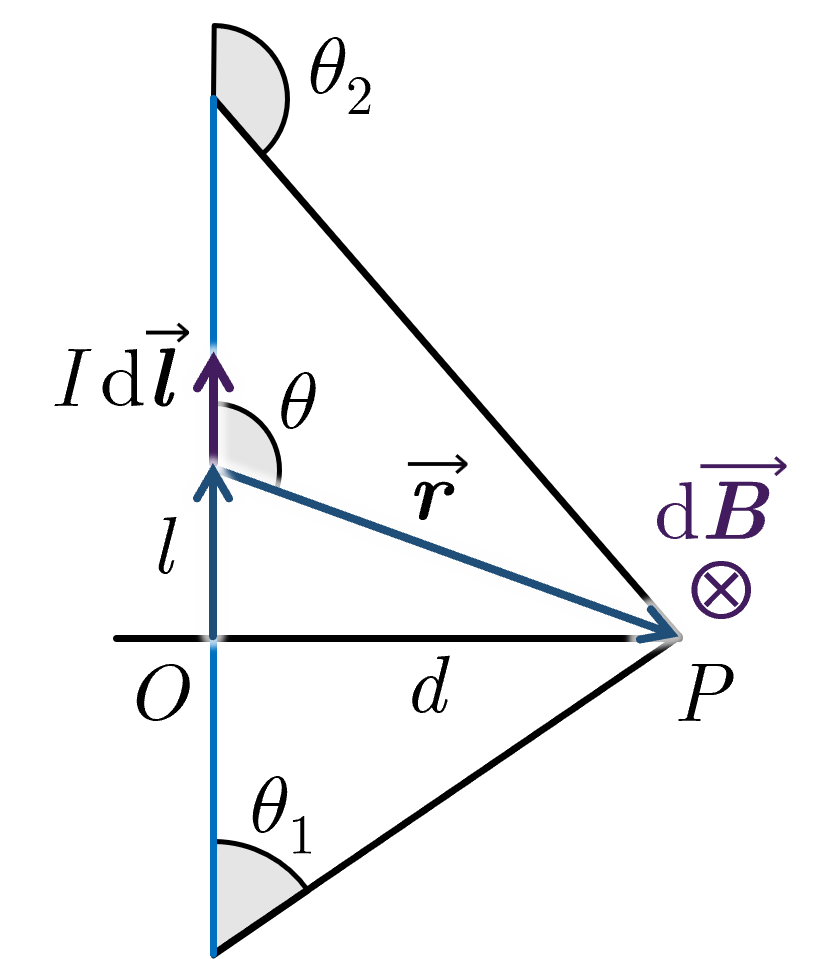
\includegraphics[width=2.95cm]{长直电流磁场.png}
		\vspace{-0.5em}
	\end{center}
	把直电流分为无数电流元,任取一电流元$I\dif \v{l}$,它在$\vr$处产生的磁场$\dif \v{B}$的大小为
	$\dif B = \dfrac{\mu_0}{4\pi}\dfrac{I\dif l\sin\theta}{r^2}$,方向垂直纸面。
	由此知所有电流元在空间同一点产生的磁场方向相同,于是对空间中一点$P$,$B = \dint \dfrac{\mu_0}{4\pi} \dfrac{I\dif l\sin\theta}{r^2}$。又由图$r=\dfrac{d }{\sin \theta}$,$l=-\dfrac{d }{\tan \theta}$,得$\dif l = \dfrac{d }{\sin^2\theta} \dif \theta$,于是 
	\begin{equation*}
		B = \dint \dfrac{\mu_0}{4\pi} \dfrac{I\dif l\sin\theta}{r^2} 
		= \dint \dfrac{\mu_0}{4\pi} \cfrac{I\dfrac{d }{\sin^2\theta} \dif \theta\sin\theta}{\dfrac{d^2 }{\sin^2 \theta}}
		= \dfrac{\mu_0I}{4\pi d} \dint \sin\theta\dif \theta
		= \dfrac{\mu_0I}{4\pi d}\left( \cos\theta_1 - \cos\theta_2 \right) 
		\qedhere
	\end{equation*}
\end{solution}
\noindent 对无限长直电流,$\theta_1=0,\theta_2=\pi$,有
\begin{equation}
	B=\dfrac{\mu_0I}{2\pi d} \label{equ: 长直电流的磁场}
\end{equation}
\end{example}

\begin{example}
	求圆电流轴线上的磁场分布。
\begin{solution}
	\adjline
	假设情境及各物理量所设如图。
	\begin{center}
		\vspace{-0.5em}
		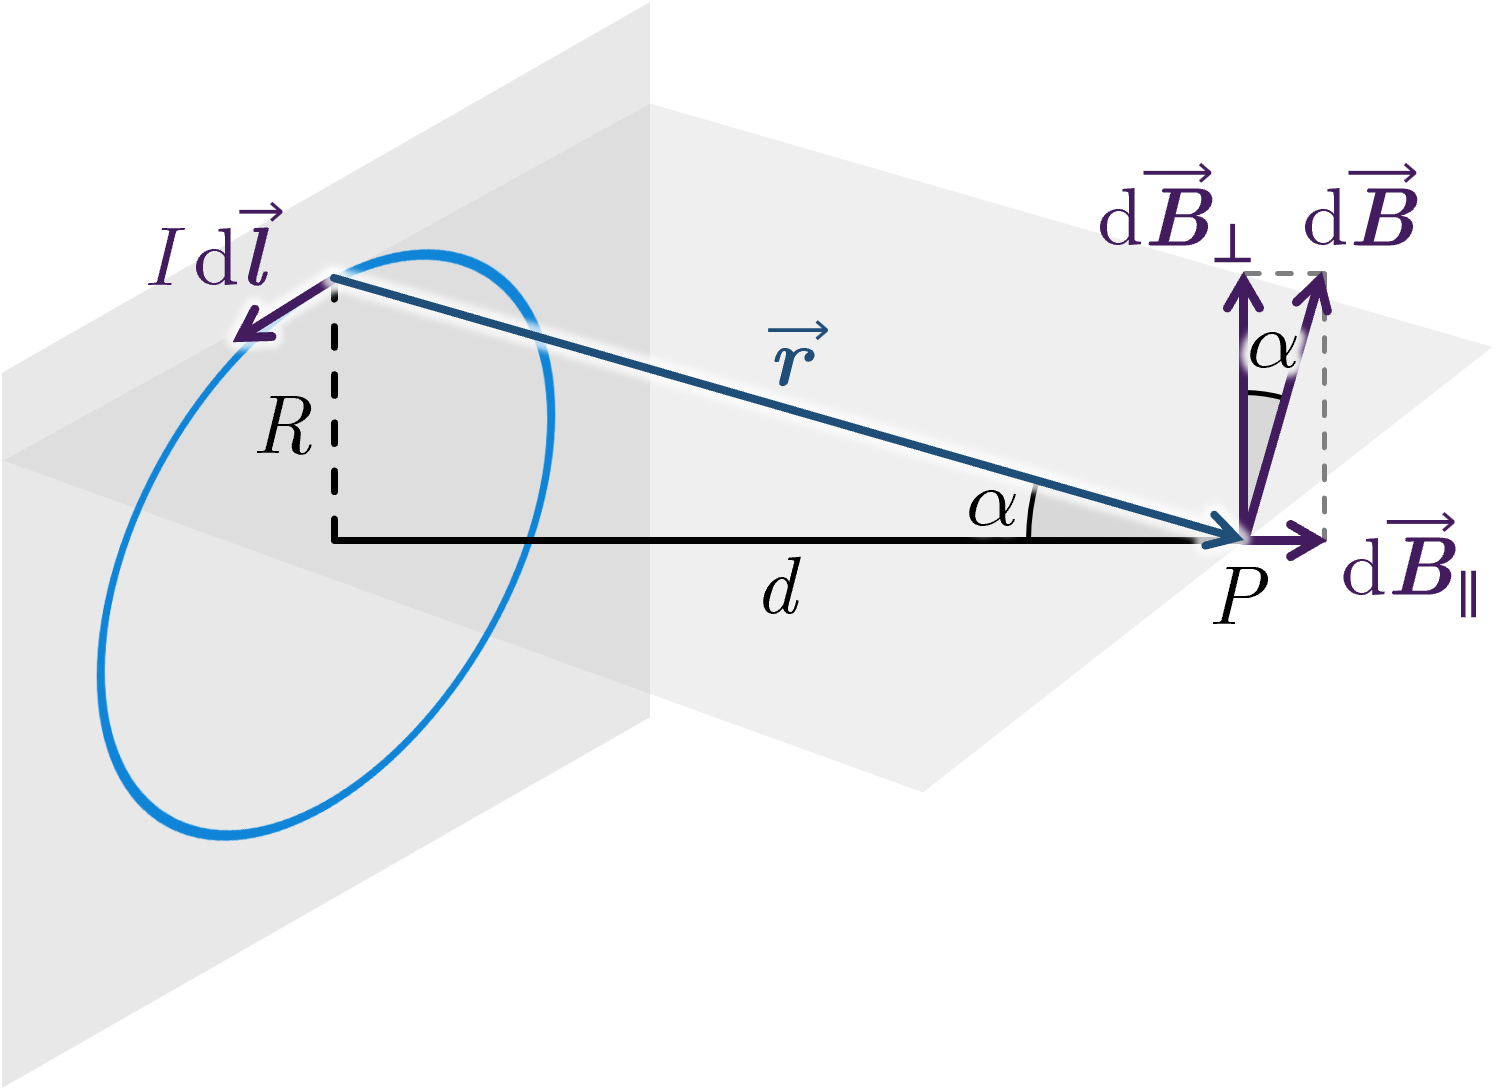
\includegraphics[width=5.87cm]{圆电流磁场.png}
		\vspace{-0.5em}
	\end{center}
	在圆电流上任取一电流元$I\dif \v{l}$,它在轴上$P$点产生的磁场$\dif \v{B}$的大小为$\dif B = \dfrac{\mu_0}{4\pi}\dfrac{I\dif l}{r^2}$,其沿轴分量为$\dif B_\parallel = \dif B \sin \alpha = \dfrac{R }{r }\dif B$,垂直于轴分量为$\dif B_\perp = \dif B \cos \alpha = \dfrac{d}{r} \dif B$。

	考虑所有电流元在$P$点的贡献,沿轴分量$\dif \v{B}_\parallel$均同向,则
	\begin{equation*}
		B_{\parallel}=\int\dif B_{\parallel}=\int\frac{\mu_{0}I\dif l}{4\pi r^{2}}\frac{R}{r}=\frac{\mu_{0}IR}{4\pi r^{3}}\int\dif l=\frac{\mu_{0}IR^{2}}{2r^{3}}
	\end{equation*}
	每一对位置对称的电流元在$P$点产生的$\dif B_\perp$对消,即$\v{B}_{\perp}=\displaystyle\int\dif \v{B}_{\perp}=\v{0}$。故 
	\begin{equation*}
		B = B_{\parallel} = \dfrac{\mu_{0}IR^{2}}{2r^{3}} = \dfrac{\mu_{0}IR^{2}}{2(R^2+d^2)^\frac{3}{2}}
	\end{equation*}
	方向沿轴线上右手螺旋所指向的方向。
\end{solution}
\noindent 在圆电流中心处,有
\begin{equation}
	B=\dfrac{\mu_0I }{2R }
\end{equation}
当$d \gg R$时,有$B = \dfrac{\mu_0 I R^2}{2d^3} = \dfrac{\mu_0 I S}{2\pi d^3}$,其中$S$为圆电流的面积。
\begin{definition}
	一个载流闭合线圈就是一个\textbf{磁偶极子},其\textbf{磁偶极矩}或\textbf{磁矩}定义为$\v{m} = I\v{S} = IS \vu*{n}$,$\vu*{n}$指向电流圈的正法线方向,即线圈电流右手螺旋所指向的方向。
\end{definition}
由此,在距离磁偶极子很远处,即当$d \gg R$时,有
\begin{equation}
	\v{B} = \dfrac{\mu_0 I\v{S}}{2\pi d^3} = \dfrac{\mu_0 \v{m}}{2\pi d^3}
\end{equation}
\end{example}

\begin{example}
	已知密绕长直螺旋线圈长为$L$,半径为$R$,线圈上单位长匝数为$n$,线圈中电流为$I$,求线圈轴线上任一点$P$的磁感强度。
\begin{solution}
	\adjline
	在密绕情形下,螺旋线圈可看作由很多圆形线圈紧密排列而成,如下图。
	\begin{center}
		\vspace{-0.5em}
		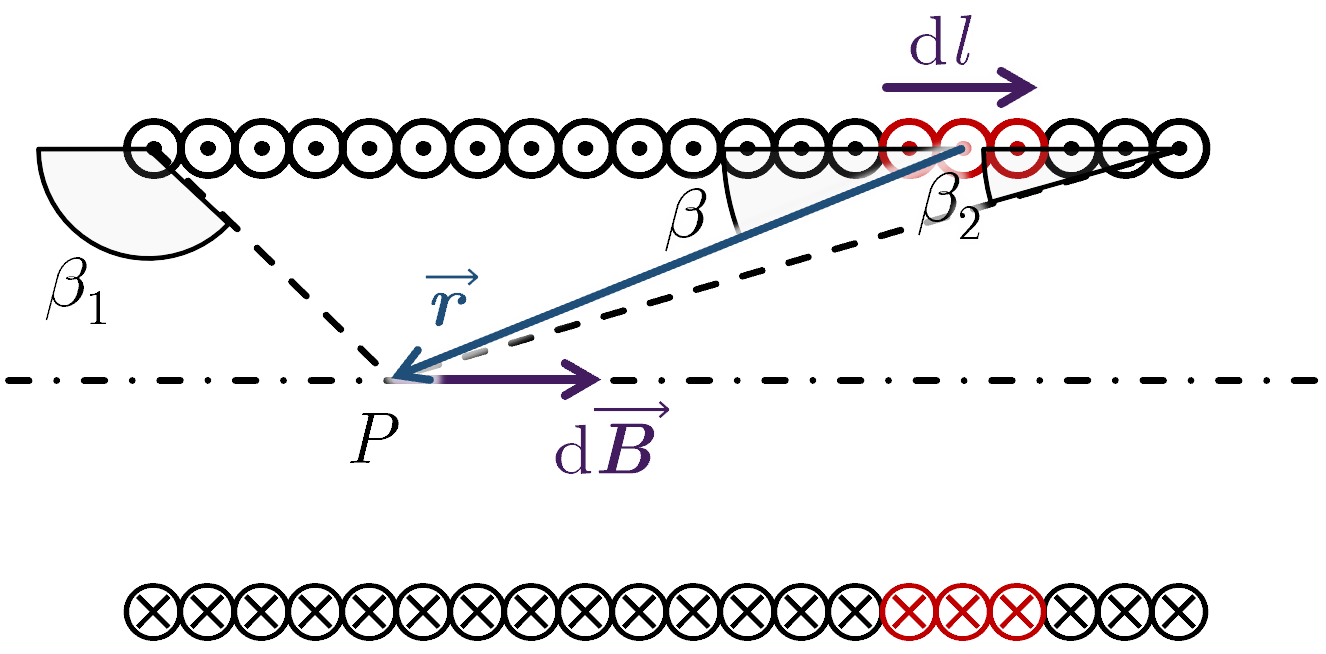
\includegraphics[width=5.87cm]{螺线管磁场.png}
		\vspace{-0.5em}
	\end{center}
	在距$P$点为$l$的地方,取长为$\dif l$的元段,其上有$n \dif l$匝线圈,相当于$\dif I=nI \dif l$的圆电流,在$P$点产生的磁感应强度大小为$\dif B = \dfrac{\mu_{0}R^{2}nI\dif l}{2(R^2+l^2)^\frac{3}{2}}$。各个元段在$P$点产生的磁感强度方向相同,整个螺旋线圈在$P$点产生的磁感强度即
	$B = \dint \dif B$。

	由图可知$\tan \beta = \dfrac{R }{l }$,即$\dif l = - \dfrac{R \dif\beta}{\sin^2\beta}$,且$\sin\beta = \dfrac{R}{(R^2+l^2)^\frac{1}{2}}$,于是 
	\begin{equation*}
		B = \int \dif B 
		= \int \dfrac{\mu_{0}R^{2}nI\dif l}{2(R^2+l^2)^\frac{3}{2}} 
		= \int_{\beta_1}^{\beta_2} \cfrac{-\mu_{0}R^{2}nI \dfrac{R \dif\beta}{\sin^2\beta}}{2\dfrac{R^3}{\sin^3\beta}} 
		= \dfrac{\mu_{0}nI }{2} \int_{\beta_1}^{\beta_2} -\sin\beta \dif\beta 
		= \dfrac{\mu_{0}nI }{2} (\cos\beta_2 - \cos\beta_1) \qedhere
	\end{equation*}
\end{solution}
\noindent 对无限长直螺线管,$\beta_1 = \pi,\beta_2 = 0$,则其轴线上任意一点处(例~\ref{e.g: 长直螺线管内}~将证明内部不在轴线上也同样成立)都有\begin{equation}
	B=\mu_0nI
\end{equation}
对半无限长直螺线管,在其端部圆心则有
\begin{equation}
	B=\dfrac{\mu_{0}nI }{2}
\end{equation}
\end{example}

\zhu[运动电荷产生的磁场]{
	毕—萨定律中电流元产生的磁场,实质上是电流元中的运动电荷产生的磁场。电流元$I\dif \v{l}$用其中载流子$q$的漂移速度$\vv$可表示为$I\dif\v{l} = nS\dif l \cdot q\vv$,其中$nS\dif l$为电流元中的运动电荷数,则每个运动电荷产生的磁场为
	\begin{equation*}
		\v{B} = \cufrac{\,\dfrac{\mu_0 I\dif\v{l} \cp \ur}{4\pi r^2}\,}{nS\dif l} = \cufrac{\,\dfrac{\mu_0 nS\dif l \cdot q\vv \cp \ur}{4\pi r^2}\,}{nS\dif l} = \dfrac{\mu_0 q\vv \cp \ur}{4\pi r^2}
	\end{equation*}
	注意,这是低速($v \ll c$)情形下匀速运动点电荷产生的磁场。电流元的磁场是稳恒场,而运动电荷的场空间分布随时间变化。运动电荷的场需要严格的相对论理论处理,涉及电磁场的洛仑兹变换。
}

\paragraph{安培环路定理}

类似于静电场的环路定理,磁场中有

\di[安培环路定理]{
	在恒定电流的磁场中,磁感强度$\v{B}$沿任何闭合路径$L$的线积分(环量)等于路径$L$所环绕的电流强度的代数和的$\mu_0$倍,即
	\begin{equation}
		\displaystyle \oint_L \v{B}\cdot\dif\v{l} = \mu_0 \sum I_\text{内}
	\end{equation}
}

\noindent 其中所谓\textbf{「环绕」}是指,设想闭合路径$L$为一根绳子,绳子勒紧后能把电流捆住。电流正方向与$L$绕向($\dif \v{l}$方向)遵循右手螺旋定则。

安培环路定理只适用于稳恒电流(闭合或伸展到$\infty$)。不同于静电场的环路定理,$\displaystyle \oint_L \v{B}\cdot \dif \v{l} \neq 0$,表面磁场为非保守场,称为\textbf{涡旋场}。

\begin{example}[2]
	求载流无限长圆柱面电流内外的磁场。设圆柱面半径为$R$,通有恒定电流$I$。
\begin{solution}
	\adjline
	由于圆柱面上电流分布的轴对称性,可知柱面外任一点的磁场均垂直于相应的$r$方向;且距离轴线同远的场点,其磁场的大小相同。

	选在垂直于轴线的平面内的过$P$点的以$r$为半径的圆形环路$L$,环路正方向与电流遵循右手螺旋定则,则 
	\begin{equation*}
		\oint_L \v{B} \cdot \dif \v{l} = B \cdot 2\pi r = \mu_0I_\text{内} 
		\quad\Longrightarrow\quad
		B = \dfrac{\mu_0}{2\pi r}I_\text{内} = \begin{cases}[ll]
			\dfrac{\mu_0I}{2\pi r},& r>R,\\
			0,& 0<r<R
		\end{cases} \qedhere
	\end{equation*}
\end{solution}
\end{example}

\begin{example}
	求载流无限长直螺旋线圈内的磁场。设线圈上单位长匝数为$n$,线圈中电流为$I$。\label{e.g: 长直螺线管内}
\begin{solution}
	因螺旋线圈无限长,并由电流分布的对称性,可知$P$点的磁场和轴线上的磁场同向,即螺旋线圈内的磁感线是一组平行于轴线的直线;且距轴线同远的点其磁场大小相同。可选如图矩形环路$L$,其上有
	\[	\oint_L \v{B} \cdot \dif \v{l} 
		= \int_a^b \v{B}_\text{轴} \cdot \dif\v{l} + \int_c^d \v{B}(r) \cdot \dif\v{l} = 0
	\]
	得\(B_\text{轴}l_{ab} - B(r)l_{cd} = 0\),即\(B(r) = B_\text{轴} = \mu_0nI\)。
\end{solution}
\end{example}

\subsubsection{磁力的规律}

\paragraph{磁场对运动电荷的作用}

由定义~\ref{磁感应强度},即有
\di[洛伦兹力]{
	以速度$\vv$运动的点电荷$q$,在磁感应强度为$\v{B}$的磁场中受到的洛伦兹力为
	\begin{equation}
		\v{F} = q\vv \cp \v{B}
	\end{equation}
}
在均匀磁场中,可将$\vv$按磁场方向分解为$v_\parallel$和$v_\perp$。平行于磁场的分量保持不变,垂直于磁场的分量在洛伦兹力$q\vv \cp \v{B}$的作用下做圆周运动,半径$R=\dfrac{mv_\perp }{qB}$,周期$T=\dfrac{2\pi m}{qB}$,故带电粒子的轨迹为轴线沿磁场方向的螺旋线,半径$R=\dfrac{m}{qB}v_\perp$,螺距$h=\dfrac{2\pi m}{qB}v_\perp$。

在非均匀磁场中,速度方向和磁场不同的带电粒子也要做螺旋运动,但半径和螺距都不断发生变化。假设粒子具有一向磁场较强处的分速度,它受到的磁场力就有一个和前进方向相反的分量。这一分量有可能最终使粒子的前进速度减小到零,并继而沿反方向前进。

\begin{eg}{霍尔效应}
	\adjline
	在一个宽度为 $h$、厚度为 $b$金属窄条中通以电流,可认为电流是外加电场$E$作用于电子使之向右作定向运动形成的,电子漂移速度为$\vv$。当加以外磁场 $\v{B}$ 时,由于洛伦兹力的作用,电子的运动将向下偏,当它们跑到窄条底部时,由于表面所限, 它们不能脱离金属因而就聚集在窄条的底部,同时在窄条的顶部显示出有多余的正电荷。这些多余的正、负电荷将在金属内部产生一横向电场$\v{E}_\mathrm{H}$。随着底部和顶部多余电荷的增多,这一电场也迅速地增大到它对电子的作用力$(-e)\v{E}_{\mathrm{H}}$与磁场对电子的作用力$(-e)\v{v}\times \v{B}$相平衡,此后电子将恢复原来水平方向的漂移运动,电流恢复为恒定电流。平衡条件为
	$$	-e\v{E}_\mathrm{H}+(-e)\v{v}\times\v{B}=\v{0}
		\quad\Longrightarrow\quad
		E_{\mathrm{H}}=vB
	$$
	由于横向电场$E_\mathrm{H}$的出现,在导体的横向两侧会出现\textbf{霍尔电压}
	$$	U_\text{H}=E_\text{H}h=vBh	$$
	已知电子的漂移速度$v$,则电流$I=nSqv=nbhqv$,其中$n$为载流子数密度。由此式求出$v$代入上式可得
	$$	U_\text{H}=vBh=\dfrac{BI}{nbq}\xlongequal{K_\mathrm{H}:=\frac{1}{nq}}K_\mathrm{H}\dfrac{BI}{b}	$$
	其中$K_\mathrm{H}$称为\textbf{霍尔系数}。
\end{eg}

\paragraph{磁场对载流导线的作用}

由定义~\ref{磁感应强度},即有
\di[安培力]{
	电流元$I \dif\v{l}$在磁感应强度为$\v{B}$的磁场中受到的安培力为
	\begin{equation}
		\dif\v{F} = I\dif\v{l} \cp \v{B}
	\end{equation}
}

\begin{example}[1]
	求两平行无限长载流直导线单位长度所受的作用力。
\begin{solution}
	\adjline
	电流$I_1$在$I_2$处产生的磁场为$B_1 = \dfrac{\mu_0I_1}{2\pi d}$,载有电流$I_2$的导线单位长度受此磁场的安培力即为
	\begin{equation*}
		\dfrac{\dif F_2}{\dif l} = B_1I_2 = \dfrac{\mu_0I_1I_2}{2\pi d}
	\end{equation*}
	当电流$I_1$在$I_2$方向相同时,两导线相吸;相反时,相排斥。
\end{solution}
\end{example}

\paragraph{磁场对磁矩的作用}

对圆电流圈(或任意平面电流线圈),其在均匀磁场中受的磁力矩为
\begin{equation}
	\v{M} = I\v{S} \cp \v{B} = \v{m} \cp \v{B}
\end{equation}


\subsection{磁场中的磁介质}

\begin{abstract}
	\item[原子和分子的磁矩] 
	\item[磁化强度] 在各向同性的顺磁质、抗磁质内,磁化强度\(\v{M} = (\mu_\mathrm{r}-1)\dfrac{1}{\mu_o\mu_\mathrm{r}}\v{B}\),磁化率\(\chi_\mathrm{m} = \mu_\mathrm{r}-1\),磁介质中磁化电流 \(I' = \oint_L \v{M} \cdot \dif \v{l}\),表面上面束缚磁化电流密度\(\v{\jmath}' = \v{M}_\text{表} \cp \vu*{n}\)。
	\item[磁场强度] 在各向同性的顺磁质、抗磁质内,磁场强度\(\v{H} = \dfrac{\v{B}}{\mu_0} - \v{M} = \dfrac{\v{B}}{\mu_0\mu_r} = \dfrac{\v{B}}{\mu}\)。
	\item[\(\v{H}\)的环路定理] 沿任一闭合路径的磁场强度的环流,等于该闭合路径所套连的传导电流的代数和,即
		\(\displaystyle \oint_L \v{H} \cdot \dif \v{l} = \textstyle \sum I_\text{0\,内}\)
	\item[磁场的界面关系]
\end{abstract}

在考虑物质受磁场的影响或其对磁场的影响时,物质统称\tboba{磁介质}。在空间中充入各种磁介质,实验发现磁介质内的磁场有的比真空时弱,有的比真空时强。
充入后与充入前磁感应强度的比值,定义为磁介质的\tboba{相对磁导率},用$\mu_\mathrm{r}$表示。依据$\mu_\mathrm{r}$的大小,可将磁介质分为3类:
\begin{itemize}
	\item \textbf{抗磁质}\quad\(\mu_\mathrm{r} < 1\),如铋、热解石墨等;
	\item \textbf{顺磁质}\quad\(\mu_\mathrm{r} > 1\),如氧等;
	\item \textbf{铁磁质}\quad\(\mu_\mathrm{r} \gg 1\),如铁、镍合金等;
\end{itemize}

\subsubsection{原子和分子的磁矩}

\paragraph{电子的磁矩}

由于电子带电,电子绕原子核作轨道运动,就相当于一个闭合载流线圈,其\tboba{轨道磁矩}为
\begin{equation}
	m=IS = -\dfrac{v}{2\pi r}e \cdot \pi r^2 = -\dfrac{e}{2m_e} \cdot m_evr = -\dfrac{e}{2m_e}L \label{equ: 电子轨道磁矩}
\end{equation}
其中\(r\)为电子的经典轨道半径,\(L\)为电子轨道运动的角动量。式~(\ref{equ: 电子轨道磁矩})~对一个原子中所有电子的总轨道磁矩也成立,这时总轨道角动量\(L\)只能取约化普朗克常量\(\hbar\)的整数倍。

电子还有自旋运动,\tboba{自旋磁矩}和自旋角动量 \(S\)的关系为
\begin{equation}
	m = -\dfrac{e }{m_e }S 
\end{equation}
代入\(S=\dfrac{\hbar}{2}\)即得\(m = -9.27 \cp 10^{-24}\mathrm{\,J/T}\),这一磁矩称为\textbf{玻尔磁子}。

\paragraph{原子核的磁矩}

原子核的磁矩可分为质子、中子分别的轨道磁矩和自旋磁矩。质子的轨道磁矩为\(m = \dfrac{e }{2m_\mathrm{p} }L\);中子不带电,轨道磁矩为0。质子和中子都有自旋磁矩\(m = g\dfrac{e }{2m_\mathrm{p}}S\),其中\textbf{\(\boldsymbol{g}\)因子}取值为在质子中\(g=5.5857\),在中子中\(g=-3.8261\)。整个\tboba{原子核的自旋磁矩}为
\begin{equation}
	m = g\dfrac{e}{2m_\mathrm{p}}I
\end{equation}
其中\(I\)为核的自旋角动量,因子\(g\)由原子核结构决定。

由上各式及\(m_e\)与\(m_\mathrm{p}\)之间的悬殊差异,可知核磁矩远小于电子磁矩。除开核磁共振情境下要单独考虑核磁矩外,通常情况下,计算原子的磁矩只计算其电子轨道和自旋磁矩即可。
\vspace{1em}

一个分子的磁矩是其中所有电子的轨道磁矩和自旋磁矩以及原子核的磁矩的矢量和。对分子整体,可以在分子磁矩\(\v{m}_\text{分}\)的意义下等效出分子电流\(i_\text{分}\),即\(\v{m}_\text{分} = i_\text{分}\v{S}_\text{分}\)。

\setcounter{paragraph}{0}
\paragraph{顺磁质的分子磁矩}

顺磁质的分子磁矩\(\v{m}_\text{分} \neq \v{0}\),称为\tboba{分子固有磁矩}。一般情况下,由于分子的热运动,\(\v{m}_\text{分}\)完全是混乱的,不显磁性。但是,在外磁场中,\(\v{m}_\text{分}\)会发生转向而整齐排列,这就是顺磁质的\tboba{磁化},如图~\ref{Pic: 顺磁质}~所示。外磁场越强,转向排列越整齐。

排列整齐的分子等效电流\(i_\text{分}\)的方向使顺磁质内部的磁场加强。顺磁质会被磁铁吸引。

\begin{figure}[!ht]
	\centering
	\vspace{-1em}
	\subfloat[顺磁质]{\label{Pic: 顺磁质}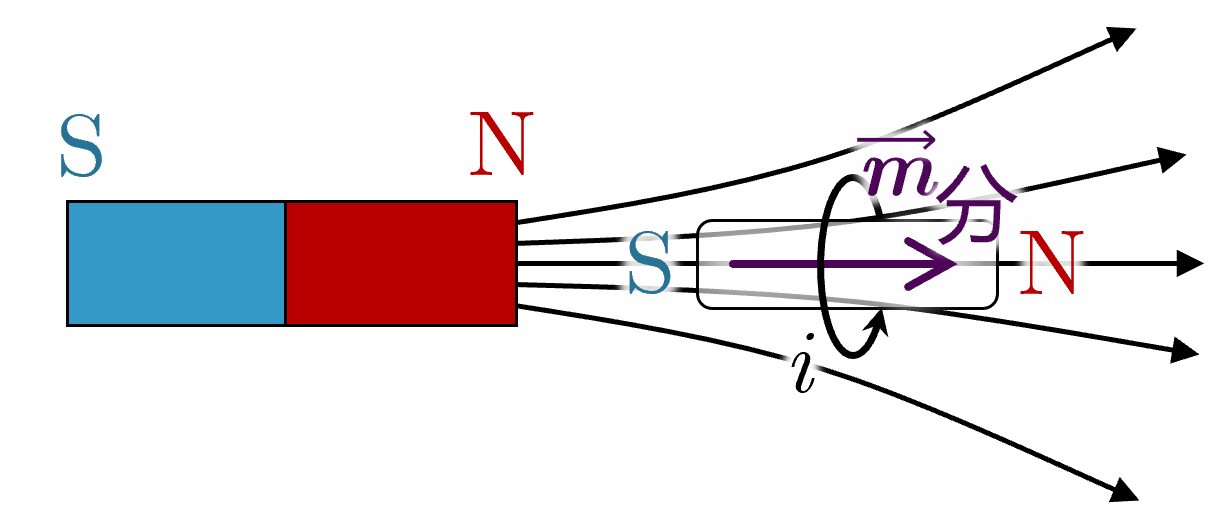
\includegraphics[width=4.55cm]{顺磁质.png}}
	\qquad
	\subfloat[抗磁质]{\label{Pic: 抗磁质}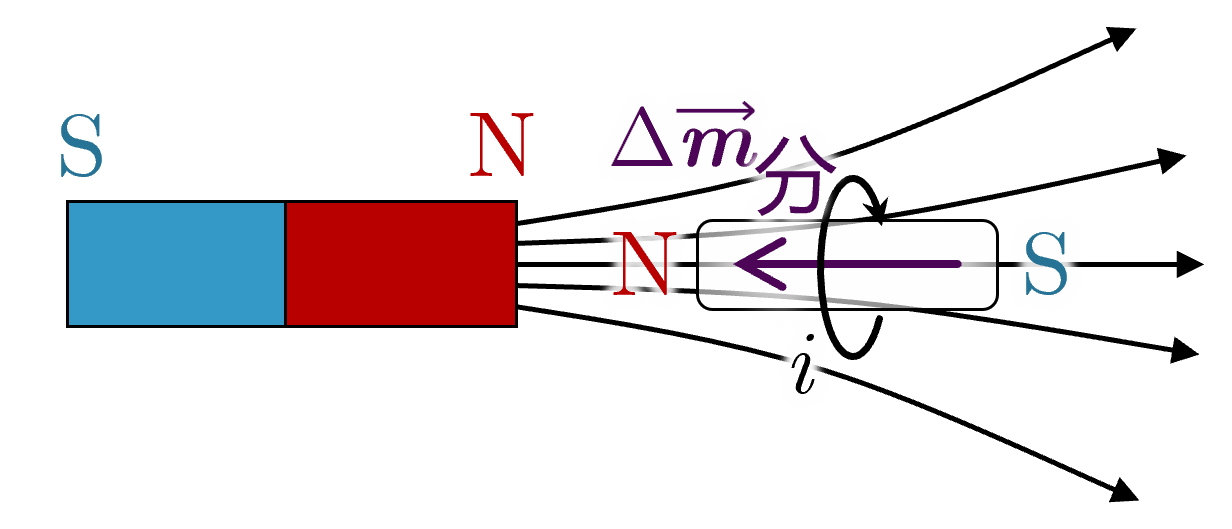
\includegraphics[width=4.55cm]{抗磁质.png}}
	\caption{分子磁矩与磁场的相互作用}
	\vspace{-0.5em}
\end{figure}

\paragraph{抗磁质的分子磁矩}

抗磁质的分子磁矩\(\v{m}_\text{分} = \v{0}\),但是在外磁场中会产生\tboba{感应磁矩}。以分子中某个电子的轨道运动为例,设该电子的轨道运动角动量为\(\v{L}\),轨道磁矩为\(\v{m}_e\),该磁矩在外磁场\(\v{B}\)中受到力矩\(\v{M}=\v{m}_e \cp \v{B}\),于是这个磁矩会发生进动。轨道进动附加的角动量与\(\v{B}\)的方向一致,所以这一进动相应的轨道磁矩(感应磁矩)\(\Delta \v{m}_e\)是与\(\v{B}\)反向的,如图~\ref{Pic: 抗磁质}~所示。因此,在抗磁质内部的磁场是被削弱的,而且抗磁质会被磁铁排斥。

\begin{figure}[!ht]
	\centering
	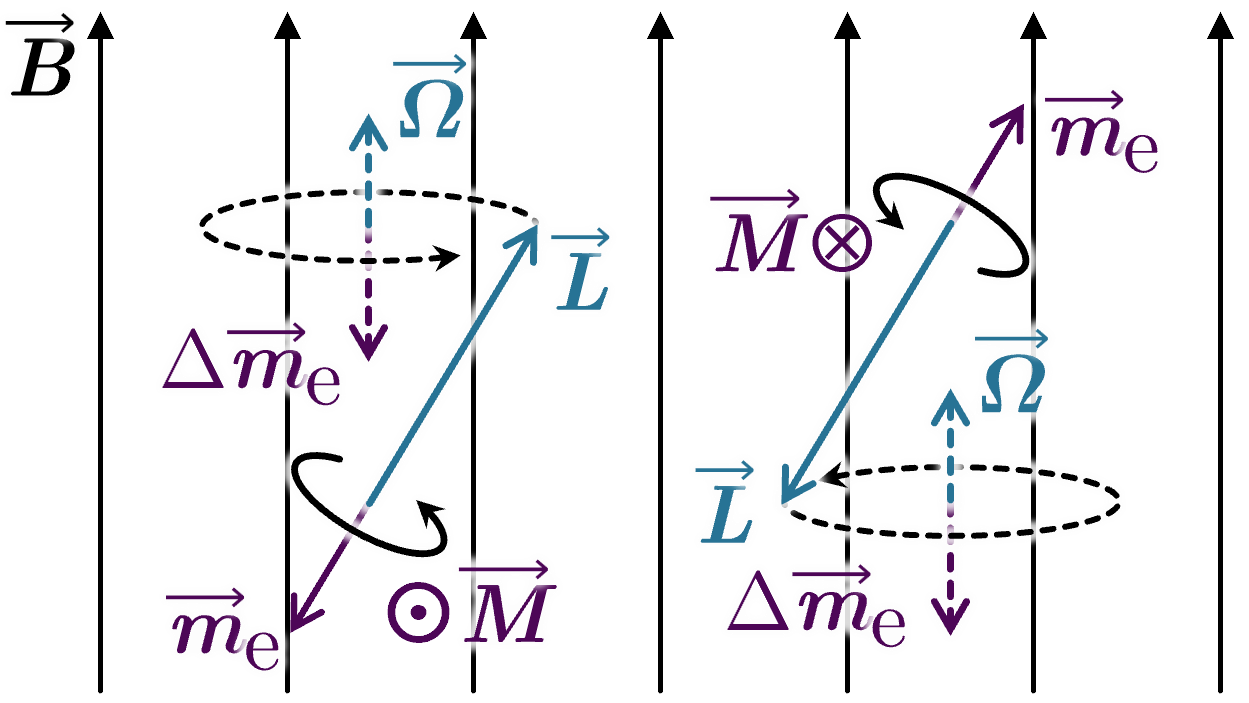
\includegraphics[width=5.5cm]{感生磁矩.png}
	\caption{抗磁质的感应磁矩}
\end{figure}

\subsubsection{磁介质的磁化}

\de[磁化强度]{
	单位体积磁介质内分子磁矩的矢量和称为磁介质中该处的\tboba{磁化强度},记作\(\v{M}\),即
	\begin{equation}
		\v{M} := \dfrac{\sum\limits_i \v{m}_{i\text{分}}}{\Dif V}
	\end{equation}
	\vspace{-1em}
}

\di[磁化强度与磁感应强度的关系]{
	在各向同性的顺磁质、抗磁质内,磁化强度\(\v{M}\)与磁感应强度\(\v{B}\)有线性关系
	\begin{equation}
		\v{M} = (\mu_\mathrm{r}-1)\dfrac{1}{\mu_o\mu_\mathrm{r}}\v{B}
	\end{equation}
	\tcblower
	\hang[3]\textbf{式中\quad}$\mu_0$——真空磁导率,取$\dfrac{\mu_0}{4\pi} = 10^{-7}\,\mathrm{T\cdot m/A}$;\\
	\(\mu_\mathrm{r}\)——磁介质的相对磁导率。
}

在外磁场作用下,磁介质出现磁性或磁性发生变化的现象称为\tboba{磁化}。在均匀磁场中,对均匀的磁介质,内部分子的磁矩整齐排列,各点处的小分子电流相互抵消,表面上的小分子电流方向相同而没有抵消,相当在表面上产生了一层\textbf{表面电流}流过,称为\tboba{磁化电流}或\tboba{束缚电流},记作\(I\)。对顺磁质和铁磁质,磁化电流产生的磁场是加强磁介质内部原磁场的;对抗磁质,磁化电流产生的磁场是削弱磁介质内部原磁场的。\textbf{磁化电流\(\boldsymbol{I'}\)是磁介质磁化的结果,其大小反映了磁化的强弱。}因此,可以考察磁化电流与磁化强度的关系。

以顺磁质为例,设磁介质中等效分子圆电流为 \(i\),半径为 \(r\),
分子磁矩为\(\v{m}_\text{分}\),其内部某点处的\(\v{M}\)(\(\v{B}\))如图~,在该点处任取小矢量元\(\dif\v{l}\),记\(\theta = \langle \v{M},\dif\v{l} \rangle\)。易知,与\(\dif\v{l}\)铰链的分子电流,其中心都位于以\(\dif\v{l}\)为轴、以\(\pi r^2\)为底面积的小柱体内。设单位体积内的分子数为\(n\),则与\(\dif\v{l}\)铰链的总分子电流为
\begin{equation*}
	\dif I' = n(\pi r^2 \cdot \dif l \cdot \cos\theta)i = nm_\text{分} \cdot \dif l \cdot \cos\theta = \v{M} \cdot \dif\v{l}
\end{equation*}
\di[磁化电流与磁化强度的基本关系]{
	设磁介质中磁化强度\(\v{M}\),则通过闭合曲线\(L\)所包围的面的磁化电流为
	\begin{equation}
		I' = \oint_L \v{M} \cdot \dif \v{l}
	\end{equation}
}
特别地,若\(\dif\v{l}\)在磁介质的表面上,可以看出某些表面会有\textbf{磁化面电流}~\(\dif I'\)。
\begin{definition}
	在垂直磁化面电流方向的单位长度上的磁化面电流,称为\textbf{\textup{面束缚磁化电流密度}},记作\(\v{\jmath}'\),即\(j' = \dfrac{\dif I'}{\dif l} \)。
\end{definition}
面束缚磁化电流密度\(\v{\jmath}'\)与磁化强度\(\v{M}_\text{表}\)的关系为 
\begin{equation*}
	j' = \dfrac{\dif I'}{\dif l} = \dfrac{\v{M}_\text{表} \cdot \dif\v{l}}{\dif l} = M_\text{表} \cos\langle \v{M}_\text{表},\dif\v{l} \rangle
	\quad\Longrightarrow\quad
	\v{\jmath}' = \v{M}_\text{表} \cp \vu*{n}
\end{equation*}
其中\(\vu*{n}\)为表面的外法向量。

\subsubsection{\(\v{H}\)\,的环路定理}

当有磁介质存在时,传导电流\(I_\text{0\,内}\)产生的磁场\(\v{B}_0\)会在磁介质中产生束缚电流\(I_\text{内}'\),束缚电流又产生磁场\(\v{B}'\),空间中任意一点的磁场强度即为\(\v{B} = \v{B}_0 + \v{B}'\),有安培环路定理\(\displaystyle \oint_L \v{B} \cdot \dif \v{l} = \mu_0 \left(\sum I_\text{0\,内} + \sum I_\text{内}'\right)\)。用\(\sum I_\text{内}' = \displaystyle \oint_L \v{M} \cdot \dif\v{l}\)代入,得
\begin{equation*}
	\oint_L \v{B} \cdot \dif \v{l} = \mu_0 \sum I_\text{0\,内} + \mu_0 \oint_L \v{M} \cdot \dif\v{l}
	\quad\Longrightarrow\quad
	\oint_L \left( \dfrac{\v{B}}{\mu_0} - \v{M} \right) \cdot \dif \v{l} = \sum I_\text{0\,内}
\end{equation*}
\de[磁场强度]{
	空间中某点处的\tboba{磁场强度}定义为
	\begin{equation}
		\v{H} = \dfrac{\v{B}}{\mu_0} - \v{M}
	\end{equation}
}
若磁介质各向同性,即有\(\v{H} = \dfrac{\v{B }}{\mu_0} - \v{M } = \dfrac{\v{B }}{\mu_0} - (\mu_\mathrm{r}-1)\dfrac{1}{\mu_o\mu_\mathrm{r}}\v{B} = \dfrac{\v{B}}{\mu_0\mu_r} = \dfrac{\v{B}}{\mu}\)。由\(\v{H}\),也可得到磁化强度\(\v{M} = (\mu_\mathrm{r}-1)\dfrac{1}{\mu_o\mu_\mathrm{r}}\v{B} = (\mu_\mathrm{r}-1)\v{H} = \chi_\mathrm{m} \v{H}\),其中\(\chi_\mathrm{m} = \mu_\mathrm{r}-1\)称为\textbf{磁化率}。
\din[\(\v{H}\)的环路定理]{
	沿任一闭合路径的磁场强度的环流,等于该闭合路径所套连的传导电流的代数和,即
	\begin{equation}
		\oint_L \v{H} \cdot \dif \v{l} = \sum I_\text{0\,内}
	\end{equation}
}

\begin{example}
	一均匀密绕细螺绕环,\(n=103\,\mathrm{m^{-1}}\),\(I=2\,\mathrm{A}\),充满\(\mu = 5 \cp 10^{-4}\,\mathrm{T\cdot m/A}\)的磁介质。求磁介质内的\(\v{H},\v{B},\v{M}\)及表面磁化电流面密度\(\v{\jmath}'\)。
	\begin{solution}
		注意到\(\mu_\mathrm{r} = \dfrac{\mu}{\mu_0} = \dfrac{5 \cp 10^{-4}}{4\pi \cp 10^{-7}} \approx 398\),即该磁介质为铁磁质。取环路\(L\)为螺环内部的同心圆,在\(L\)上各点处应有\(\v{H},\v{B},\v{M}\)都沿\(L\)的方向,则由环路定理
		\begin{equation*}
			\oint_L \v{H} \cdot \dif\v{l} = H \cdot 2\pi r = 2\pi rn\cdot i
		\end{equation*}
		于是\(H=nI=2000\,\mathrm{A/m}\),\(B=\mu H=1\,\mathrm{T }\),\(M=(\mu_\mathrm{r}-1)H = 7.94 \cp 10^5\,\mathrm{A/m}\),\(j'=M_\text{表}=7.94 \cp 10^5\,\mathrm{A/m}\)。
	\end{solution}
\end{example}

\subsubsection{磁场的界面关系}

在介质分界面上,作一扁筒式封闭面为高斯面\(\varSigma\),面积为\(\Dif S\)的两底面分别在两介质内并平行于界面,则由\(\v{B}\)的高斯定律可得
\begin{align*}
	\varoiint_{\varSigma} \v{B} \cdot \dif \v{s} &= \v{B}_1 \cdot \Dif S\vu*{n} + \v{B}_2 \cdot \Dif S (-\vu*{n}) \\[-10pt] 
	&= \bigl(\v{B}_1 \cdot \vu*{n} - \v{B}_2 \cdot \vu*{n}\bigr) \Dif S
	= (B_{1\mathrm{n}}-B_{2\mathrm{n}}) \Dif S = 0 
	\quad\Longrightarrow\quad B_{1\mathrm{n}}-B_{2\mathrm{n}} = 0
\end{align*}
即 
\begin{equation}
	B_{1\mathrm{n}} = B_{2\mathrm{n}},\qquad 
	\dfrac{H_{1\mathrm{n}}}{H_{2\mathrm{n}}} = \dfrac{\mu_2}{\mu_1}
\end{equation}
类似地,在介质分界面上作一窄条矩形环路\(\varGamma\),长度为\(\Dif L\)的两长边分别在两介质内并平行于界面,则由\(\v{H}\)环路定理可得
\begin{align*}
	\oint_\varGamma \v{H} \cdot \dif \v{l} 
	&= \v{H}_1 \cdot \Dif L \vu*{\tau} + \v{H}_2 \cdot \Dif L (-\vu*{\tau}) \\[-10pt] 
	&= \bigl(\v{H}_1 \cdot \vu*{\tau} - \v{H}_2 \cdot \vu*{\tau}\bigr) \Dif L
	= (H_{1\uptau}-H_{2\uptau}) \Dif L = \sum I_\text{0\,内}
	\quad\Longrightarrow\quad H_{1\uptau}-H_{2\uptau} = \dfrac{\sum I_\text{0\,内}}{\Dif L}
\end{align*}
在交界面无自由电流的情形下,即有 
\begin{equation}
	H_{1\uptau}=H_{2\uptau},\qquad 
	\dfrac{B_{1\uptau}}{B_{2\uptau}} = \dfrac{\mu_1}{\mu_2}
\end{equation}

\subsection{电磁感应}

\subsubsection{法拉第电磁感应定律}

\di[楞次定律]{
	感应电流的磁通总是\tbome{阻碍}原磁通的变化;导体在磁场中运动时,导体中出现的感应电流所受到的磁场力必然\tbome{阻碍}此导体的运动。
}
\di[法拉第电磁感应定律]{
	闭合回路的感应电动势\(\mathscr{E}\)和穿过回路的磁通\(\varPhi\)的时间变化率成正比,即 
	\begin{equation}
		\mathscr{E} = - \dt[\varPhi]
	\end{equation}
	其中,\(\mathscr{E }\)的正方向与回路中所选的正方向一致,\(\varPhi\)的正方向与回路正方向成右手螺旋关系。
}

进而,当\(N\)匝线圈串联时,总感应电动势应是各圈回路感应电动势之和。
\de[全磁通、磁链]{
	导电线圈或电流回路中,穿过各匝线圈的磁通量的总和称为\tboba{全磁通},记作\(\varPsi\),即 
	\begin{equation}
		\varPsi = \sum\limits_i \varPhi_i
	\end{equation}
	当穿过各匝线圈的磁通量相等时,全磁通\(\varPsi = N\varPhi_i\)称为\tboba{磁链}。
}
\begin{theorem}
	\textbf{\textup{线圈的法拉第电磁感应定律\quad}}闭合线圈的感应电动势\(\mathscr{E}\)和穿过线圈的全磁通\(\varPsi\)的时间变化率成正比,即 
	\begin{equation}
		\mathscr{E} = - \dt[\varPsi]
	\end{equation}
	其中,\(\mathscr{E }\)的正方向与回路中所选的正方向一致,\(\varPsi\)的正方向与回路正方向成右手螺旋关系。
\end{theorem}

由\(\varPhi = \v{B} \cdot \v{S}\),代入可知
\begin{equation*}
	\mathscr{E} = - \dt[(\v{B} \cdot \v{S})] = - \v{B} \cdot \dt[\v{S}] - \dt[\v{B}] \cdot \v{S}
\end{equation*}

\paragraph{动生电动势\(\mathscr{E}_\text{动} = - \v{B} \cdot \dt[\v{S}]\)}

导体在磁场中运动时,导体中的自由电荷在洛仑兹力作用下定向移动,产生感应电动势,这就是动生电动势。

对于直导线在均匀磁场中运动的情况,有
\(\mathscr{E}_\text{动} =  - \v{B} \cdot \dt[\v{S}] = - B_\perp \cdot l \dt[x_\perp] = - B_\perp l v_\perp \),其中\(v_\perp\)的正方向应是垂直于直导线、使回路面积增大的方向。

更一般地,对规定了正方向的小段直导线\(\dif \v{l}\),有
\(\dif \mathscr{E}_\text{动} = \v{B} \cdot (\dif\v{l} \cp \dt[\v{x}]) = \v{B} \cdot (\dif\v{l} \cp \vv) = (\vv \cp \v{B}) \cdot \dif\v{l}\),故
\di[动生电动势的计算]{
	在恒定磁场中,导线路径\(L\)的动生电动势为
	\begin{equation}
		\mathscr{E}_\text{动} = \int_L \left( \vv \cp \v{B} \right) \cdot \dif\v{l}
	\end{equation}
}
动生电动势的本质,是通过洛仑兹力实现能量转换。

\begin{eg}{交流发电机}
	交流发电机中,线圈与磁极相对转动,有 
	\begin{align*}
		\mathscr{E} = - N \dt[\varPhi] = - N \dt[\big( \v{B} \cdot \v{S} \big)]
		= - N \dt[\bigl(BS\cos(\omega t + \varphi_0)\bigr)] = \omega NBS \sin(\omega t + \varphi_0)
	\end{align*}
	即电动势的峰值\(\mathscr{E}_m = \omega NBS\),其中\(N\)为线圈匝数,\(\varphi = \omega t + \varphi_0\)是线圈平面的正法向量与磁场的夹角。通常取初始夹角\(\varphi_0 = 0\),即初始线圈平面与磁场方向垂直,有\(\mathscr{E} = \mathscr{E}_m \sin \omega t\)。
\end{eg}

\paragraph{感生电动势\(\mathscr{E}_\text{感} = - \dt[\v{B}] \cdot \v{S}\)}
静止回路所在的磁场发生变化时,回路包围的磁通变化,在回路中会产生感应电动势,这就是感生电动势。

感生电动势产生的原因,是变化的磁场激发了空间中的感生电场。感生电场的电力线是闭合的,是一种非静电场。正是这种非静电场产生了感生电动势。由电动势的普遍定义知
\begin{equation*}
	\oint_L \v{E}_\text{感} \cdot \dif \v{l} = \mathscr{E}_\text{感} 
	= - \iint_S \dfrac{\partial \v{B}}{\partial t} \cdot \dif\v{s}
	\quad\Longleftrightarrow\quad
	\v{\nabla} \cp \v{E}_\text{感} = - \dfrac{\partial \v{B}}{\partial t}
\end{equation*}
\din[修正的\(\v{E}\)的环路定理,label=E的环路定理]{
	沿任一闭合路径的电场强度的环流,等于该闭合路径包围的曲面上磁感应强度变化率的通量的相反数,即 
	\begin{equation}
		\oint_L \v{E} \cdot \dif \v{l} = - \iint_S \dfrac{\partial \v{B}}{\partial t} \cdot \dif\v{s}
	\end{equation}
}

\begin{example}
	电子感应加速器是利用感生电场来加速电子的一种设备,它的柱形电磁铁在两极间产生磁场,在磁场中安置一个环形真空管道作为电子运行的轨道。当磁场发生变化时,就会沿管道方向产生感生电场,射入其中的电子就受到这感生电场的持续作用而被不断加速。
	
	设环形真空管的轴线半径为\(a\),求磁场变化时沿环形真空管轴线的感生电场。
	\begin{solution}
		\adjline
		由磁场分布的轴对称性可知,感生电场的分布也具有轴对称性。沿环管轴线上各处的电场强度大小应相等,而方向都沿轴线的切线方向。因而沿此轴线的感生电场的环路积分为
		$$\oint_L E_\mathrm{i}\cdot\dif r=E_\mathrm{i} \cdot 2\pi a$$
		以$\overline{B}$ 表示环管轴线所围绕的面积上的平均磁感应强度,则通过此面积的磁通量为
		$$\varPhi=\overline{B}S=\overline{B} \cdot \pi a^2$$
		于是
		$$E_\mathrm{i} \cdot 2\pi a=-\frac{\dif \varPhi}{\dif t}=-\pi a^2\frac{\dif \overline{B}}{\dif t}$$
		由此
		\begin{equation*}
			E_\mathrm{i}=-\frac{a}{2}\frac{\dif \overline{B}}{\dif t} \qedhere
		\end{equation*}
	\end{solution}

	感应加速器中,随时间变化的磁场\(\v{B}(t)\)身兼双职:
	\begin{itemize}
		\item \(\v{B}(t)\)对电子施加的洛仑兹力作为圆周轨道的向心力;
		\item 时变磁场所激发的感生电场\(\v{E}_\mathrm{i}\)使电子在做圆周运动时不断被加速。
	\end{itemize}
	要保证电子做加速圆周运动,则磁场不是均匀磁场,且需要满足\(B_\text{轨道}(t) = \dfrac{1}{2} \overline{B}(t)\)。
\end{example}

\subsubsection{互感与自感}

\begin{definition}
    一个回路中的电流变化时,其所产生的磁场在它附近的另一回路中产生的感生电动势称为\textbf{互感电动势}。
\end{definition}

对两个固定线圈,假设线圈1 中的电流 \(i_1\) 随时间 \(t\) 变化,在线圈2中产生的互感电动势为\(\mathscr{E}_{21}\)。由 Biot-Savart定律,知\(i_1\)的磁场\(B_1 \propto i_1\),从而\(i_1\)在线圈2中的全磁通\(\psi_{21} \propto i_1\),即可定义其比例系数\(M_{21} := \dfrac{\psi_{21}}{i_1}\),称为\textbf{线圈1对线圈2的互感(系数)}。这样,线圈1中的电流在线圈2中产生的感应电动势就为\(\mathscr{E}_{21} = - \dt[\varPsi_{21}] = - M_{21} \dt[i_1]\)。同理,也会有定义\(M_{12} := \dfrac{\psi_{12}}{i_2}\),有结论\(\mathscr{E}_{12} = - \dt[\varPsi_{12}] = - M_{12} \dt[i_2]\)。可以证明,\(M_{12} = M_{21}\)。

\de[互感(系数)]{
	两个固定线圈中,任意一个上单位电流在另一线圈中产生的全磁通,称为这两个线圈之间的\tboba{互感(系数)}\!\!,记作\(M\),即
	\begin{equation}
		M = \dfrac{\psi_{21}}{i_1}= \dfrac{\psi_{12}}{i_2}
	\end{equation}
}
\di[线圈的互感]{
	给定两个固定线圈,则其任意一个线圈中的电流在另一线圈中产生的互感电动势,大小上等于该电流变化率与互感系数的乘积,即 
	\begin{equation}
		\mathscr{E}_{21} = - M_{21} \dt[i_1],\qquad \mathscr{E}_{12} = - M_{12} \dt[i_2]
	\end{equation}
}

\begin{definition}
	一个线圈的电流发生变化时,通过线圈自身的全磁通也会发生变化,线圈内产生的感生电动势称为\textbf{自感电动势}。
\end{definition}

\de[自感(系数)]{
	线圈中通有单位电流强度时,通过线圈自身的全磁通的大小,称为这个线圈的\tboba{自感(系数)}\!\!,记作\(L\),即
	\begin{equation}
		L = \dfrac{\psi}{i}
	\end{equation}
}
则可知,\(\mathscr{E}_\text{自} = - \dt[\psi] = - L \dt[i]\)。自感电动势总是阻碍回路电流的变化。

两个线圈的自感与它们的互感之间的关系为
\begin{equation}
	M=k\sqrt{L_1L_2}
\end{equation}
其中\(k\)为\textbf{耦合系数},\(0 \le k \le 1\)。

\subsubsection{磁场的能量}

自感为$L$ 的线圈中通有电流$I$ 时所储存的磁能应该等于这电流消失时自感电动势所做的功。这个功可如下计算。以$i\dif t$表示在短路后某一时间 $\dif t$内通过负载的电量,则在这段时间内自感电动势做的功为
$$\dif A=\mathscr{E}_L i\dif t=-L\frac{\dif i}{\dif t}i\dif t=-Li\dif i$$
电流由起始值减小到零时,自感电动势所做的总功就是
$$A=\int\dif A=\int_I^0-Li\dif i=\frac{1}{2}LI^2$$
这也就是自感为$L$ 的线圈中通有电流$I$ 时的磁能\(W_\mathrm{m}\)。电感能量储存在磁场中,那么对一个长直螺线管来说,\(L = \dfrac{\psi}{i} = \cufrac{N \cdot B \cdot \dfrac{\pi d^2}{4}}{i} = \cufrac{N \cdot \dfrac{\mu N i}{l} \cdot \dfrac{\pi d^2}{4}}{i} = \dfrac{\pi\mu N^2d^2}{4l} = \mu n^2 Sl = \mu n^2 V\),即\(W_\mathrm{m} = \dfrac{1}{2} \mu n^2 V I^2 = \dfrac{B^2}{2\mu} V\)。

\de[磁场能量密度]{
	单位体积磁场所具有的能量,称为\tboba{磁场能量}(的体积)\tboba{密度},记作$w_\mathrm{m}$。
}
\di[磁场能量与磁场强度的关系]{
	磁场能量密度$w_\mathrm{m}$与该处磁场强度$H$的平方成正比,比例系数为磁导率$\mu$的一半,即
	\begin{equation}
		w_\mathrm{m} = \dfrac{\mu H^2}{2} = \dfrac{B^2}{2\mu}
	\end{equation}
}


\subsection{Maxwell电磁理论}

\subsubsection{全电流假说}

对于非稳恒电流的情况,Maxwell 提出了一个重要假设:电容器充电时其内存在\textbf{位移电流},它和传导电流总体是连续的。

由电流连续性方程\(\displaystyle \varoiint_S \v{J}_\text{传} \cdot \dif\v{s} = - \dfrac{\dif Q_\text{内}}{\dif t}\)(定理~\ref{电流连续性方程}),
而\(Q_\text{内}=\displaystyle \varoiint_S \v{D} \cdot \dif \v{s}\)(高斯定理),
即得\(\displaystyle \varoiint_S \v{J}_\text{传} \cdot \dif\v{s} = - \varoiint_S \dfrac{\partial \v{D}}{\partial t} \cdot \dif \v{s}\),
也即\(\displaystyle \varoiint_S \left( \v{J}_\text{传} + \dfrac{\partial \v{D}}{\partial t} \right) \cdot \dif\v{s} = 0\)。
相应地,\(\dfrac{\partial \v{D}}{\partial t}\)称为\textbf{位移电流密度},记作\(\v{J}_\text{位}\)。

\din[修正的\(\v{H}\)的环路定理, label=H的环路定理]{
	沿任一闭合路径的磁场强度的环流,等于该闭合路径所套连的传导电流和位移电流的代数和,即
	\begin{equation}
		\oint_L \v{H} \cdot \dif \v{l} = I_\text{传内} + I_\text{位内}
	\end{equation}
	\tcblower
	\hang[3]\textbf{式中\quad}$I_\text{传内}$——与\(L\)套连的传导电流的代数和,\(I_\text{传内} = \displaystyle \iint_S \v{J} \cdot \dif\v{s}\);\\
	\(I_\text{位内}\)——与\(L\)套连的位移电流的代数和,\(I_\text{位内} = \dt[\varPhi_D] = \displaystyle \dt \iint_S \v{D} \cdot \dif\v{s} = \iint_S \dfrac{\partial \v{D}}{\partial t} \cdot \dif\v{s}\)。
}

\begin{example}
	半径为 \(R = 0.1\mathrm{\,m}\) 的两块圆形平板电容器,
	两板间距为\(d \ll R\),充电过程中某时刻两板
	之间电场的时间变化率为\(\dt[E] = 10^{13}\mathrm{\,V/m}\)。求此时刻:

	(1)两板间的位移电流;

	(2)两板间距中心轴线\(r_1 = 0.02\mathrm{\,m }\)处、\(r_2 = 0.12\mathrm{\,m }\)处的磁感应强度。

	\begin{solution}
		\adjline
		(1)由\(d \ll R\),忽略边缘效应,板间电场均匀。
		\begin{equation*}
			I_\text{位} = \dt[\varPhi_D] = \pi R^2 \cdot \dt[D] = \pi R^2 \varepsilon_0 \dt[E] = 2.78\mathrm{\,A}
		\end{equation*}

		(2)全电流对中心轴是对称的,它产生的磁场对中心轴也是对称的。作半径为\(r_1\)、\(r_2\)的回路\(L_1\)、\(L_2\),方向与电场方向成右手螺旋,显然前者在两板所成柱体之内,后者在柱外。
		
		对\(L_1\)由\(\v{H}\)的环路定理,
		\begin{equation*}
			\oint_{L_1} \v{H}_1 \cdot \dif \v{l} = I_\text{位1} = \iint_{S_1} \dfrac{\partial \v{D}}{\partial t} \cdot \dif\v{s} = \iint_{S_1} \dfrac{\partial D}{\partial t} \cdot \dif s
		\end{equation*}
		即
		\begin{equation*}
			H_1 \cdot 2\pi r_1 = \varepsilon_0 \dt[E] \pi r_1^2
			\quad\Longleftrightarrow\quad 
			H_1 = \dfrac{\varepsilon_0 r_1}{2} \dt[E]
		\end{equation*}
		于是\(B_1 = \mu_0 H_1 = \dfrac{\mu_0\varepsilon_0 r_1}{2} \dt[E] = 1.11 \cp 10^{-6} \mathrm{\,T}\)。

		同理,对\(L_2\)由\(\v{H}\)的环路定理,
		\begin{equation*}
			\oint_{L_2} \v{H}_2 \cdot \dif \v{l} = I_\text{位2} = \iint_{S_2} \dfrac{\partial \v{D}}{\partial t} \cdot \dif\v{s} = \iint_{S_2} \dfrac{\partial D}{\partial t} \cdot \dif s
		\end{equation*}
		即
		\begin{equation*}
			H_2 \cdot 2\pi r_2 = \varepsilon_0 \dt[E] \pi R^2
			\quad\Longleftrightarrow\quad 
			H_2 = \dfrac{\varepsilon_0 R^2}{2r_2} \dt[E]
		\end{equation*}
		于是\(B_2 = \mu_0 H_2 = \dfrac{\mu_0\varepsilon_0 R^2}{2r_2} \dt[E] = 4.64 \cp 10^{-6} \mathrm{\,T}\)。
	\end{solution}
	注意到 
	\begin{equation*}
		B_\text{外} = \mu_0 H_\text{外} = \dfrac{\mu_0\varepsilon_0 R^2}{2r} \dt[E]
		= \dfrac{\mu_0}{2\pi r} \pi R^2 \dt[(\varepsilon_0E)]
		= \dfrac{\mu_0}{2\pi r} I_\text{位}
	\end{equation*}
	这与例~\ref{e.g: 长直电流的磁场}~的集中于轴线上的长直电流\( I_\text{传} \)的磁场(式~(\ref{equ: 长直电流的磁场}))是一样的规律。
\end{example}

\subsubsection{Maxwell方程组}

定理~\ref{D的高斯定理}、定理~\ref{E的环路定理}、定理~\ref{B的高斯定理}~和定理~\ref{H的环路定理}~组成 Maxwell方程组。

\di[Maxwell方程组]{
	空间中的电磁场满足
	\begin{equation}
		\text{\tbome{微分形式}}
		\begin{cases}
			\v{\nabla} \cdot \v{D} = \rho_0 \\
			\v{\nabla} \cp \v{E} = -\dfrac{\partial \v{B}}{\partial t} \\
			\v{\nabla} \cdot \v{B} = 0 \\
			\v{\nabla} \cp \v{H} = \v{\jmath}_0 + \dfrac{\partial \v{D}}{\partial t}
		\end{cases}
		\qq{或}
		\text{\tbome{积分形式}}
		\begin{cases}
			\displaystyle \varoiint_S \v{D} \cdot \dif\v{s} = \iiint \rho_0 \dif\mu \\[5pt]
			\displaystyle \oint_L \v{E} \cdot \dif\v{l} = -\iint_S \dfrac{\partial \v{B}}{\partial t} \cdot \dif\v{s}\\[8pt]
			\displaystyle \varoiint_S \v{B} \cdot \dif\v{s} = 0 \\[5pt]
			\displaystyle \oint_L \v{H} \cdot \dif\v{l} = \iint_S \bigg( \v{\jmath}_0 + \dfrac{\partial \v{D}}{\partial t} \bigg) \cdot \dif\v{s}
		\end{cases}
	\end{equation}
}

由方程组出发,Maxwell预言:变化的电磁场将以波的形式传播。

\paragraph{电磁波的速度}

令\(j_0=0,\rho_0=0\),对沿\(x\)方向传播的电磁场可导出
\[\dfrac{\partial^2 E_y}{\partial x^2} = \mu\varepsilon \dfrac{\partial^2 E_y}{\partial t^2},\qquad \dfrac{\partial^2 H_z}{\partial x^2} = \mu\varepsilon \dfrac{\partial^2 H_z}{\partial t^2}\]
与标准波动方程\(\dfrac{\partial^2 \xi}{\partial x^2} = \dfrac{1}{v^2} \dfrac{\partial^2 \xi}{\partial t^2}\)比较,即知电磁波的波速\(v=\dfrac{1}{\sqrt{\mu\varepsilon}}\)。真空中,此式即为
\begin{equation}
	c = \dfrac{1}{\sqrt{\mu_0\varepsilon_0}}
\end{equation}
\begin{theorem}
	真空中的一列电磁波中,电场成分\(\v{E}\)、磁场成分\(\v{B}\)与波速\(\v{c}\)的关系为
	\begin{equation}
		\v{E} = \v{B} \cp \v{c} \qq{或} \v{B} = \dfrac{\v{c} \cp \v{E}}{c^2}
	\end{equation}
\end{theorem}

\paragraph{电磁场的能量}

在空间某点处,电磁场的能量密度(单位体积内电磁场的能量)为
\begin{equation*}
	w=w_\mathrm{e}+w_\mathrm{m} = \dfrac{1}{2}\varepsilon E^2 + \dfrac{1}{2\mu} B^2
\end{equation*}
由\(\v{E} = \v{B} \cp \v{c}\),即知有\(w_\mathrm{m} = \dfrac{1}{2\mu} \left( \dfrac{E}{c} \right)^2 = \dfrac{1}{2\mu} \dfrac{E^2}{(\mu\varepsilon)^{-1}} = \dfrac{1}{2}\varepsilon E^2 = w_\mathrm{e}\)。因此\(w=\varepsilon E^2 = \dfrac{B^2}{\mu} \)。

电磁波传播时,电磁场的能量也跟着传播。
\begin{definition}
	\textbf{\textup{电磁波的能流密度矢量}\quad}表征空间中一点处电磁波在单位时间单位面积上的能量传播的矢量,称为\textbf{电磁波的能流密度矢量},也称\textbf{\textup{Poynting}矢量},记作\(\v{S}\)。\textup{Poynting}矢量的大小等于单位时间内通过垂直于传播方向的单位面积的电磁波的能量,方向为该点处电磁波的传播方向。
\end{definition}
由定义,知
\begin{align*}
	\v{S} = \dfrac{w\cdot \v{c}\dif t \cdot \dif A}{\dif A \cdot \dif t} = w\v{c} = \varepsilon \v{E}^2 \v{c} = \varepsilon \v{E} \cdot (\v{B} \cp \v{c}) \cdot \v{c} = \varepsilon (\v{E} \cp \v{B}) \v{c}^2 =  \varepsilon (\v{E} \cp \v{B}) \dfrac{1}{\mu\varepsilon} = \v{E} \cp \v{H}
\end{align*}


\newpage
%----------------------------------------------------------
\appendix
\section{必要的数学准备}

\subsection{矢量运算}

\subsubsection{矢量乘法}

\de[矢量的标量积(点乘)]{
	两个矢量的\tboba{标量积}~$\v{A} \cdot \v{B}$是一个标量,定义为$\v{A} \cdot \v{B} := AB\cos \theta$,其中$0 \le \theta \le \upi$为$\v{A}$与$\v{B}$的夹角。
}
点乘满足交换律,因其不封闭而不满足结合律,对矢量的线性运算满足分配律。

\de[矢量的矢量积(叉乘)]{
	两个矢量的\tboba{矢量积}~$\v{A} \cp \v{B}$是一个矢量,大小定义为$\left| \v{A} \cp \v{B} \right|= AB\sin \theta$,其中$0 \le \theta \le \upi$为$\v{A}$与$\v{B}$的夹角;方向根据右手定则确定。
}
叉乘不满足交换律($\v{A} \cp \v{B} = -\v{B} \cp \v{A}$),对矢量的线性运算满足分配律。显然,对任意矢量$\v{A}$,$\v{A} \cp \v{A} = \v{0}$,于是我们规定$\v{A}^2=\v{A} \cdot \v{A}$,即$\v{A} ^2 = A^2$。

\di[矢量乘法的坐标表示]{
	在三维笛卡尔坐标系下,设两个矢量$\v{A}=\begin{bmatrix}
		A_x \\ A_y \\ A_z
	\end{bmatrix},\v{B}=\begin{bmatrix}
		B_x \\ B_y \\ B_z
	\end{bmatrix}$(或记作$\v{A}=A_x\ux + A_y\uy + A_z\uz,\v{B}=B_x\ux + B_y\uy + B_z\uz$),则
	
	(1)$\v{A} \cdot \v{B} = A_xB_x + A_yB_y + A_zB_z$;

	(2)$\v{A} \cp \v{B} = \begin{vmatrix}
		\ux & \uy & \uz \\
		A_x & A_y & A_z \\
		B_x & B_y & B_z
	\end{vmatrix} = (A_yB_z-A_zB_y)\ux + (A_zB_x-A_xB_z)\uy + (A_xB_y-A_yb_x)\uz$。
}

\di[矢量乘法的重要公式]{
	(1)$\v{A} \cdot (\v{B} \cp \v{C}) = \v{B} \cdot (\v{C} \cp \v{A}) = \v{C} \cdot (\v{A} \cp \v{B})$;

	(2)$\v{A} \cp (\v{B} \cp \v{C}) = (\v{A} \cdot \v{C}) \v{B} - (\v{A} \cdot \v{B}) \v{C}$。
}

其中,定理~\ref{矢量乘法的重要公式}(1)式具有明确的几何意义:$\left|\v{A} \cdot (\v{B} \cp \v{C})\right|$是以$\v{A},\v{B},\v{C}$为三邻边的平行六面体的体积,当$\v{A}$在$\v{B},\v{C}$按右手定则确定的一侧时可去绝对值。

\subsubsection{矢量微分}

参考实数上的定义,可以定义矢量对标量的导数。
\de[矢量对标量的导数]{
	设$\v{f}:(a,b)\rightarrow \R^n$为函数,$x_0\in (a,b)$,若
	$$\lim\limits_{x\rightarrow x_0}\frac{\v{f}(x)-\v{f}(x_0)}{x-x_0}=\lim\limits_{h\rightarrow 0}\frac{\v{f}(x_0+h)-\v{f}(x_0)}{h}$$
	存在、确定、有限,则称$\v{f}$在$x_0$处\tboba{可导},上述极限被称为函数$\v{f}$在$x_0$处的\tboba{导数},记作$\eval{\dfrac{\dif \v{f}}{\dif x}}_{x_0}$、$\mathrm{D}_x\v{f}(x_0)$等。
}

\di[矢量求导的运算法则]{
	(1)加法法则:$\dt[(\v{A}+\v{B})] = \dt[\v{A}] + \dt[\v{B}]$;

	(2)乘法法则:$\dt[(\v{A} \cdot \v{B})] = \dt[\v{A}] \cdot \v{B} + \v{A} \cdot \dt[\v{B}]$,$\dt[(\v{A} \cp \v{B})] = \dt[\v{A}] \cp \v{B} + \v{A} \cp \dt[\v{B}]$。
}

%----------------------------------------------------------
\end{document}